%for a more compact document, add the option openany to avoid
%starting all chapters on odd numbered pages
\documentclass[12pt]{cmuthesis}

% This is a template for a CMU thesis.  It is 18 pages without any content :-)
% The source for this is pulled from a variety of sources and people.
% Here's a partial list of people who may or may have not contributed:
%
%        bnoble   = Brian Noble
%        caruana  = Rich Caruana
%        colohan  = Chris Colohan
%        comar    = Cyrus Omar
%        jab      = Justin Boyan
%        josullvn = Joseph O'Sullivan
%        jrs      = Jonathan Shewchuk
%        kosak    = Corey Kosak
%        mjz      = Matt Zekauskas (mattz@cs)
%        pdinda   = Peter Dinda
%        pfr      = Patrick Riley
%        dkoes = David Koes (me)

% My main contribution is putting everything into a single class files and small
% template since I prefer this to some complicated sprawling directory tree with
% makefiles.

% link formatting
\usepackage{hyperref}
\hypersetup{
    colorlinks,
    linkcolor={red!50!black},
    citecolor={blue!50!black},
    urlcolor={blue!80!black}
}


% some useful packages
\usepackage{times}
\usepackage{fullpage}
\usepackage{graphicx}
\usepackage{amsmath}
\usepackage[numbers,sort]{natbib}
\usepackage{subfigure}
\hypersetup{
pageanchor=true,plainpages=false,bookmarksnumbered,
pdfborder=0 0 0,  %removes outlines around hyper links in online display
}

% Approximately 1" margins, more space on binding side
\usepackage[letterpaper,twoside,vscale=.8,hscale=.75,nomarginpar]{geometry}
%for general printing (not binding)
% \usepackage[letterpaper,twoside,vscale=.8,hscale=.75,nomarginpar,hmarginratio=1:1]{geometry}

%%%%%%%%%%%%%%%%%%%%%%%%%%%%%%%%%%%%%%%%%%%%%%%%%%%%%%%%%%%%%%%%%%%%%%%%%%%%%%%%
% Nimo's macros

% latin: https://tex.stackexchange.com/questions/15009/macros-for-common-abbreviations
\usepackage{xspace}
\newcommand*{\eg}{e.g.,\@\xspace}
\newcommand*{\ie}{i.e.,\@\xspace}
\newcommand*{\apriori}{a priori\@\xspace}

\makeatletter
\newcommand*{\etc}{%
    \@ifnextchar{.}%
        {etc}%
        {etc.\@\xspace}%
}
% inline figures
\usepackage{wrapfig}

% remove blank pages
\let\cleardoublepage\clearpage

% systems
\newcommand*{\Penrose}{\textsc{Penrose}\xspace}
\newcommand*{\Substance}{\textsc{Substance}\xspace}
\newcommand*{\SubstanceColored}{\colorbox[HTML]{E7F3E7}{\Substance}\xspace}

\newcommand*{\Domain}{\textsc{Domain}\xspace}
\newcommand*{\Style}{\textsc{Style}\xspace}
\newcommand*{\Edgeworth}{\textsc{Edgeworth}\xspace}

% thesis statement
\newcommand{\boxtext}[1]{\begin{center} \fbox{ \parbox{0.95\linewidth}{ #1 }} \end{center} }

% fancy ref
\usepackage[capitalise, noabbrev]{cleveref}

% figure styling
\usepackage[font=footnotesize,labelfont=bf]{caption}

% quotes
\newcommand\quotei[1]{``\textit{#1}''}

% links
\renewcommand{\UrlFont}{\ttfamily\small}

% code
\usepackage{listings}
\usepackage{xcolor}
\usepackage{realboxes}
\definecolor{sub}{HTML}{E7F3E7}
\definecolor{sty}{HTML}{DDDEED}
\definecolor{dsl}{HTML}{DBDBDB}
\newcommand\sub[1]{\Colorbox{sub}{\lstinline{#1}}}
\newcommand\sty[1]{\Colorbox{sty}{\lstinline{#1}}}
\newcommand\dsl[1]{\Colorbox{dsl}{\lstinline{#1}}}
\usepackage{listings}
\newcommand{\lstbg}[3][0pt]{{\fboxsep#1\colorbox{#2}{\strut #3}}}
\lstdefinelanguage{JavaScript}{
  morekeywords=[1]{break, continue, delete, else, for, function, if, in, new, return, this, typeof, var, void, while, with, export, default class, class, extends, constructor, Circle},
  % Literals, primitive types, and reference types.
  morekeywords=[2]{false, null, true, boolean, number, undefined,
    Array, Boolean, Date, Math, Number, String, Object},
  % Built-ins.
  morekeywords=[3]{eval, parseInt, parseFloat, escape, unescape, matmul},
%   otherkeywords={=>, =},
  sensitive, 
  morecomment=[s]{/*}{*/},
  morecomment=[l]//,
  morecomment=[s]{/**}{*/}, % JavaDoc style comments
  morecomment=[f][\lstbg{red!20}]-,
  morecomment=[f][\lstbg{green!20}]+,
  morestring=[b]',
  morestring=[b]"
}[keywords, comments, strings]
\lstdefinestyle{CodeStyle}{
  language=JavaScript,
  tabsize=2,
  showspaces=false,
  showstringspaces=false
  breaklines=true,
  aboveskip = 0pt,
  belowskip = 0pt,
}
\lstset{    
  basicstyle=\linespread{0.8}\footnotesize\ttfamily, 
  style=CodeStyle,
  columns=fullflexible
} 

% algorithm
\usepackage{algorithm}
\usepackage{algpseudocode}

% margin mark
\usepackage[color, leftbars]{changebar}
\setlength\changebarsep{10pt}
\newenvironment{proposed}
    {
    \cbcolor[HTML]{FBB040}
    \setlength\changebarwidth{6pt}
    \cbstart
    }
    {
    \cbend 
    }

% timeline
\usepackage{pgfgantt}

% edgeworth design goals
\usepackage{enumitem}

% edgeworth ui labels
% figure annotation
\usetikzlibrary{calc}
\definecolor{labelColor}{RGB}{64,81,182}
\newcommand{\uilabel}[1]{\protect\tikz [font=\sffamily, baseline={($ (current bounding box.center) - (0,.3em) $)}] \fill[fill=labelColor] (0,0em) circle (0.6em) node[text=white] {#1};}

% algorithm position
\usepackage{float}

% table
\usepackage{array} % For m{} column specifier
\usepackage{colortbl}
\usepackage{multirow}

% full page figures
\usepackage{rotating}

% Define a command to create a progress bar
\definecolor{freqColor5}{HTML}{007000}
\definecolor{freqColor4}{HTML}{238823}
\definecolor{freqColor3}{HTML}{FFBF00}
\definecolor{freqColor2}{HTML}{FF6600}
\definecolor{freqColor1}{HTML}{D2222D}

\usetikzlibrary{calc}
\newcommand{\progressbar}[1]{%
    \begin{tikzpicture}[xscale=0.2, yscale=0.2, baseline=(current bounding box.south)]
        \draw[fill=white] (0, 0) rectangle (5, 1); % Background rectangle
        \ifdim #1pt<2pt
            \draw[fill=red] (0, 0) rectangle (#1, 1); % Red for <2
        \else\ifdim #1pt<3pt
            \draw[fill=freqColor2] (0, 0) rectangle (#1, 1); % Yellow for <3
        \else\ifdim #1pt<4pt
            \draw[fill=freqColor3] (0, 0) rectangle (#1, 1); % Yellow-green for <4
        \else
            \draw[fill=freqColor5] (0, 0) rectangle (#1, 1); % Green for >=4
        \fi\fi\fi
    \end{tikzpicture}%
}

% RQs
\newcounter{rqcounter} % Define a new counter for RQs
\renewcommand{\therqcounter}{RQ\arabic{rqcounter}} % Format the counter as RQ1, RQ2, etc.

\newcounter{rqsupcounter} % Define a new sub-counter for sub-RQs
\renewcommand{\therqsupcounter}{RQ3.\arabic{rqsupcounter}} % Format the sub-counter as RQ3.1, RQ3.2, etc.
% \renewcommand{\therqsupcounter}{RQ\arabic{rqsupcounter}} % Format the sub-counter as RQ1, 2, 3 etc

% Interviews chapter imports
\usepackage{subcaption}
\newcommand\itquote[1]{\hangindent=1em\hangafter=0
``\textit{#1}''}
\newcommand{\latin}[1]{{\it #1}}




% Penrose chapter imports
\usepackage{mdframed}
\usepackage{overpic}
\newcommand{\figloc}[1]{\textit{#1}}
\usepackage{listings, multicol} % code listings w/ formatting
\lstset{keepspaces=true}

\lstdefinelanguage{Sub-LA}{
  morekeywords={Vector, VectorSpace, Scalar, LinearMap, In, Orthogonal, EqualLength, Unit, Autolabel, Label, All, Default},
  morecomment=[l][\color{gray}]{--}
}

\lstdefinelanguage{Sub-tensor}{
  morekeywords={Dim, Vector, Matrix, Scalar, Autolabel, Label, All, Default},
  morecomment=[l][\color{gray}]{--}
}

\lstdefinelanguage{Sub-nn}{
  morekeywords={Dim, Vector, Matrix, Scalar, Function, vec, softmax, L, Autolabel, Label, All, Default},
  morecomment=[l][\color{gray}]{--}
}

\lstdefinelanguage{Sub-mesh}{
  morekeywords={SimplicialComplex, Edge, Vertex, InVS, SimplicialSet, IsSubsetOf, Star, Subcomplex, SetMinus, Union, Closure, Link, Result, AutoLabel, Label, All, Default},
  morecomment=[l][\color{gray}]{--}
}

\lstdefinelanguage{Sub-geom}{
  morekeywords={Table, Chair, BeerMug, Tavern, Plate, Point, Midpoint, Bisector, Triangle, Right, Obtuse, Acute, Angle, Line, Segment, Square, Rectangle, On, Parallel, PerpendicularBisector, Ray, Disjoint, Altitude, Endpoint, On, Perpendicular},
  morecomment=[l][\color{gray}]{--}
}

\lstdefinelanguage{Sty-LA}{
  morekeywords={Vector, VectorSpace, Scalar, LinearMap, Arrow, Rectangle, Arc, Dot, AnchorPoint, CurlyBrace, Parallelogram, Line, global, forall, where, above, below, with, ensure, encourage, override, layer, ALL, CANVAS, delete},
  morecomment=[l][\color{gray}]{--}
}

\lstdefinelanguage{Elem}{
  morekeywords={type, function, notation, predicate},
  morecomment=[l][\color{gray}]{--}
}

\lstdefinelanguage{Sub-RA}{
  morekeywords={Reals, Real, Interval, Function, IsDifferentiable, IsDiscontinuous, Point, Autolabel, Pt, Label, NoLabel, All, Default},
  morecomment=[l][\color{gray}]{--}
}

\lstdefinelanguage{Sub-SET}{
  morekeywords={Autolabel, Pt, Label, NoLabel, All, Default, Set, IsSubset, NotIntersecting},
  morecomment=[l][\color{gray}]{--}
}

\lstdefinelanguage{Sty-RA}{
  morekeywords={Reals, Real, Interval, Function, Differentiable, Diff, Discontinuous, Point, Pt, LeftBounded, LeftClopen, Open, Bounded, Arrow, Rectangle, Arc, Dot, AnchorPoint, CurlyBrace, Parallelogram, Line, Tick, DoubleArrow, Bracket, Region, Curve, Paren, global, forall, where, above, below, with, ensure, encourage, override, layer, ALL, CANVAS, delete, Auto, optimized},
  morecomment=[l][\color{gray}]{--}
}

\lstdefinelanguage{Sub-RT}{
  morekeywords={Scene, In, String, HasForm, PathSample, Sample, SceneSatisfies, AutoLabel, Diagram, LightSource, Camera, PathType, Path, VertexType, BounceType, DiffuseBounce, SpecularBounce, GlossyBounce, sample, Autolabel, Pt, Label, NoLabel, All, Default},
  morecomment=[l][\color{gray}]{--}
}

\lstdefinelanguage{Sty-RT}{
  morekeywords={Diagram, LightSource, Camera, PathType, Path, VertexType, BounceType, DiffuseBounce, SpecularBounce, GlossyBounce, InList, Sublist, sample, PathVertex, Path, InVP, Hits, PathType, DiffuseObject, PathEdge, SpecularObject, Arrow, Rectangle, Arc, Dot, AnchorPoint, CurlyBrace, Parallelogram, Line, Tick, DoubleArrow, Bracket, Region, Curve, Paren, global, forall, where, above, below, with, ensure, encourage, override, layer, ALL, CANVAS, delete, Auto, optimized, plugin},
  morecomment=[l][\color{gray}]{--}
}

\lstdefinelanguage{Sub-ST}{
  morekeywords={Set, Point, Map, Intersection, Union, Subtraction, CartesianProduct, Difference, Subset, AddPoint, Apply, From, Empty, Nonempty, Intersect, Nonintersecting, IsSubset, NotSubset, PointIn, PointNotIn, Injection, Not, Surjection, Bijection, Autolabel, Label, All, Default},
  morecomment=[l][\color{gray}]{--}
}

\lstdefinelanguage{Sty-ST}{
  morekeywords={Set, Point, Map, Intersection, Union, Subtraction, CartesianProduct, Difference, Subset, AddPoint, Apply, From, Empty, Nonempty, Intersect, Nonintersecting, IsSubset, NotSubset, PointIn, PointNotIn, Injection, Surjection, Bijection, global, forall, where, above, below, with, ensure, encourage, override, layer, ALL, CANVAS, delete},
  morecomment=[l][\color{gray}]{--}
}

\lstset{
  basicstyle=\small\ttfamily,
  columns=flexible,
  breaklines=true,
  mathescape=true,
  numbers=left
}

% mdframed style for Domain code
\definecolor{DslBGColor}{rgb}{0.95,0.95,0.95}
\definecolor{DslLineColor}{rgb}{0.85,0.85,0.85}
\mdfdefinestyle{DSLCode}{
    backgroundcolor=DslBGColor,
    linecolor=DslLineColor,
    linewidth=1pt,
    innertopmargin=8pt,
    innerbottommargin=8pt,
    innerleftmargin=8pt,
    innerrightmargin=8pt
 }

% mdframed style for Substance code
\definecolor{SubBGColor}{rgb}{0.92,0.97,0.92}
\definecolor{SubLineColor}{rgb}{0.87,0.92,0.87}
\mdfdefinestyle{SUBCode}{
    backgroundcolor=SubBGColor,
    linecolor=SubLineColor,
    linewidth=1pt,
    innertopmargin=8pt,
    innerbottommargin=8pt,
    innerleftmargin=8pt,
    innerrightmargin=8pt
 }

% mdframed style for Style code
\definecolor{StyBGColor}{rgb}{0.95,0.95,1.00}
\definecolor{StyLineColor}{rgb}{0.9,0.9,0.95}
\mdfdefinestyle{STYCode}{
    backgroundcolor=StyBGColor,
    linecolor=StyLineColor,
    linewidth=1pt,
    innertopmargin=8pt,
    innerbottommargin=8pt,
    innerleftmargin=8pt,
    innerrightmargin=8pt
 }

\usepackage{tikz}
\newcommand\inlineDSL[2][]{\ \tikz[overlay]\node[draw,inner sep=2pt, anchor=text, rectangle, thick, color=DslLineColor, fill=DslBGColor, text=black,] {#2};\phantom{#2}\ }
\newcommand\inlineSUB[2][]{\ \tikz[overlay]\node[draw,inner sep=2pt, anchor=text, rectangle, thick, color=SubLineColor, fill=SubBGColor, text=black,] {#2};\phantom{#2}\ }
\newcommand\inlineSTY[2][]{\ \tikz[overlay]\node[draw,inner sep=2pt, anchor=text, rectangle, thick, color=StyLineColor, fill=StyBGColor, text=black,] {#2};\phantom{#2}\ }

\newcommand{\keyword}[1]{\texttt{\textbf{#1}}}
\usepackage{amssymb}
\usepackage{upgreek}
\newcommand{\resp}{\emph{resp.}} % "respectively"
\def\ContinueLineNumber{\lstset{firstnumber=last}}

% typewriter font
\usepackage{inconsolata} % Load the Inconsolata font
\renewcommand{\ttdefault}{zi4} % Set Inconsolata as the default typewriter font


% Goals
\newcounter{goalcounter} % Define a new counter for RQs
\renewcommand{\thegoalcounter}{Goal \arabic{goalcounter}} % Format the counter as RQ1, RQ2, etc.

% \usepackage{caption}
% \captionsetup[table] % Adjusts space between the table caption and the table


% chinese
% \usepackage{xeCJK}

%%%%%%%%%%%%%%%%%%%%%%%%%%%%%%%%%%%%%%%%%%%%%%%%%%%%%%%%%%%%%%%%%%%%%%%%%%%%%%%%


% Provides a draft mark at the top of the document. 
\draftstamp{\today}{DRAFT}

% 


\begin {document} 
\frontmatter

%initialize page style, so contents come out right (see bot) -mjz
\pagestyle{empty}

\title{ 
{\bf Developing conceptual understanding through interactive diagramming}}

\author{Wode ``Nimo'' Ni}
\date{\today}
\Year{2024}
\trnumber{CMU-S3D-24-XXX}

\committee{
Kenneth Koedinger and Joshua Sunshine, Carnegie Mellon University, Co-chairs \\
Brad Myers, Carnegie Mellon University \\
Titus Barik, Apple\\
Shriram Krishnamurthi, Brown University\\
\trnumber{}
}

% \support{}
% \disclaimer{}

% copyright notice generated automatically from Year and author.
% permission added if \permission{} given.

% \keywords{Stuff, More Stuff}

\maketitle

\begin{dedication}
To the pool gods.
\end{dedication}

\pagestyle{plain} % for toc, was empty

\begin{abstract}

TODO
% ``Mental pictures'' and ``visual intuition'' capture how people make sense of abstract concepts and see solutions to hard problems in a visual way. Learning research suggests that visual representations of knowledge are powerful tools for thought. Visual representations like diagrams enable more robust learning and flexible problem solving. 

% Existing diagramming tools often require hours of low-level tweaking of geometric primitives and do not capture the core task of diagramming: representing ideas visually. \Penrose is a diagramming platform that explicitly encodes visual representations in domain-specific languages. In this thesis proposal, I argue that this explicit encoding can be leveraged to (1) reduce the programming effort of producing diagrammatic problems at scale and (2) simplify the workflow of authoring interactive diagrams. The resulting diagrams also carry rich semantics, and I'll discuss how to use them to (3) provide useful, automated feedback to students. 


\end{abstract}

\begin{acknowledgments}
TODO
\end{acknowledgments}


\tableofcontents
% \listoffigures
% \listoftables

\mainmatter

%% Double space document for easy review:
%\renewcommand{\baselinestretch}{1.66}\normalsize

% The other requirements Catherine has:
%
%  - avoid large margins.  She wants the thesis to use fewer pages, 
%    especially if it requires colour printing.
%
%  - The thesis should be formatted for double-sided printing.  This
%    means that all chapters, acknowledgements, table of contents, etc.
%    should start on odd numbered (right facing) pages.
%
%  - You need to use the department standard tech report title page.  I
%    have tried to ensure that the title page here conforms to this
%    standard.
%
%  - Use a nice serif font, such as Times Roman.  Sans serif looks bad.
%
% Other than that, just make it look good...


% 
\chapter*{Prelude}

\vspace{-30pt}

Trigonometric identities are often presented as a big list of rules. 

\noindent\includegraphics[width=\linewidth]{assets/prelude/trig-identities.pdf}


\noindent Students are often asked to solve problems by applying a subset of those rules, \eg, $sin(0 - \theta) = -sin(\theta)$.

\begin{figure*}[h]
    \centering
    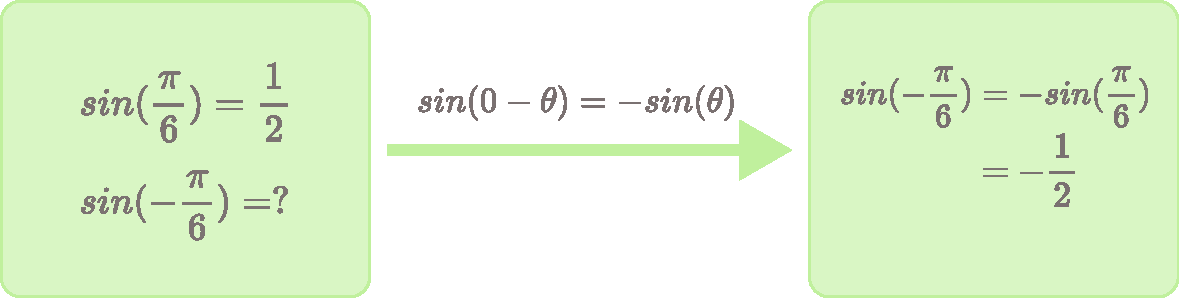
\includegraphics[width=0.75\linewidth]{assets/prelude/symbolic-transform.pdf}
    % \vspace{-10pt}
\end{figure*}

\setlength{\columnsep}{1em}
\setlength{\intextsep}{0em}
\begin{wrapfigure}{r}{.23\textwidth}
\vspace{-10pt}
  \begin{center}
    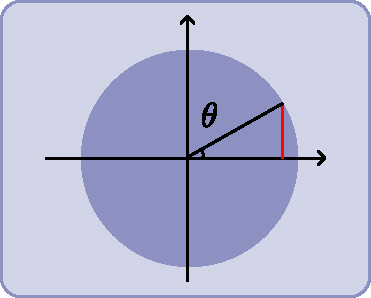
\includegraphics[width=0.23\textwidth]{assets/prelude/unit-circle.pdf}
  \end{center}
\end{wrapfigure}

A useful visual representation of this concept is the unit circle: on a Cartesian plane with a circle of radius $1$ centered at the origin, concrete values of trig functions are represented visually and rules are implicitly encoded as geometric transformations. For instance, the value of $sin(\theta)$ is the y-coordinate of a point on the circle, where the ray from the origin to the point forms angle $\theta$ with the x-axis.

To derive the identity rule visually, one only needs to note that $-\theta$ is a reflection about the x-axis, and observe that the y-coordinate is now a negative number. Instead of having to memorize a big set of rules, one can reduce this problem to a simple operation on the visual representation of a unit circle.

\vspace{10pt}
\begin{figure*}[h]
    \centering
    \includegraphics[width=0.70\linewidth]{assets/prelude/visual-transform.pdf}
    % \vspace{-10pt}
\end{figure*}

By translating the symbols to a visual representation, a unit circle, a student completely bypasses the tedious memorization of trig identities. While this is a much more retainable and robust representation for students, are we teaching representations like this to students? What does it take for students to internalize it? 

\chapter{Introduction}
\section{Motivation}
\label{sec:motivation}

``Mental pictures'' and ``visual intuition'' capture how people make sense of abstract concepts and see solutions to hard problems in a visual way. Jacques Hadamard described numerous examples of mathematicians doing exactly this in \emph{The Mathematician's Mind}~\cite{Hadamard1997a}, later summarized by Alan Kay~\cite{doingWithImages}:

\begin{quote}
Jacques Hadamard, the famous French mathematician, in the late stages of his life, decided to poll his 99 buddies, who made up together the 100 great mathematicians and physicists on the earth, and he asked them, ``How do you do your thing?'' They were all personal friends of his, so they wrote back depositions. Only a few, out of the hundred, claimed to use mathematical symbology at all. Quite a surprise. All of them said they did it mostly in imagery or figurative terms.
\end{quote}

Learning research suggests that visual representations of knowledge are powerful tools for thought. Visual representations like diagrams enable more robust learning \cite{multimediaLearning} and abstract and flexible problem solving~\cite{Koedinger1990a, pictureAlgebra,whyDiagramWorth}. Importantly, when people work with visuals, they build better conceptual understanding and more flexible mental models that go beyond memorized procedures~\cite{multipleReps}.

Creating visual representations of complex concepts involves transforming abstract ideas into tangible illustrations~\cite{coulon_importance_2024}. This process demands both a deep understanding of the subject matter and expertise in graphical tools--skills that are not commonly found together. As a result, despite the demand for diagrams, the ability to create them is limited to a small group of specialists. Consequently, much of the mathematical literature is sparsely illustrated.  As William Thurston noted, ``Mathematicians usually have fewer and poorer figures in their papers and books than in their heads.'' This sparsity of diagrams also affects students, continuing Kay's train of thought:

\begin{quote}
    The sad part of the diagram is that every child in the United States is taught math and physics through this [symbolic] channel. The channel that almost no adult creative mathematician or physicist uses to do it... They use this channel to communicate, but not to do their thing.
\end{quote}

\section{Thesis Overview}

I~\footnote{All the work presented in this proposal was carried out in collaboration with others, and to recognize this, I use ``we'' rather than the singular first person in the subsequent chapters.} investigated how domain experts create conceptual diagrams via semi-structured interviews (\cref{chp:interviews}). The study revealed that diagramming tools should be \textit{representationally salient}: tools should allow authors to define visual representations for domain-specific concepts in a manageable, scalable, and composable way. 

Existing diagramming tools often require hours of low-level tweaking of geometric primitives and do not capture the core task of diagramming: representing ideas visually. Consequently, the diagrams created by existing tools don't have semantics, as they are merely a collection of pixels and geometric blobs. Others who want to build upon existing diagrams often cannot reproduce the work, because diagrams are currently delivered in low-level formats such as rasterized images and Scalable Vector Graphics (SVG). 

To address this problem, I designed a tool called \Penrose, which supports representational salience (\cref{chp:penrose}). The \Penrose format contains the \emph{source information} of diagram design: using \Penrose, diagram authors encode domain-specific concepts and how to visually represent them in plain-text languages. \Penrose generates diagrams from this encoding through automatic layout. I demonstrate the effectiveness and generality of the system by showing how it can be used to encode visual representations across a wide range of domains.

\Penrose has several potential audiences of users. I chose to validate its usefulness for making diagrammatic problems because:

\begin{itemize}
    \item the learning sciences literature provides ample evidence for the use of them~\cite{multipleReps, multimediaLearning, cotraining}.
    \item by making diagrammatic problems using \Penrose, problem authors can inform us about the ecological validity of \Penrose-generated diagrams.
    \item problem authors is a concrete user group that have high demand for more diagrams and use them for social good.
\end{itemize}

Atop \Penrose, I built \Edgeworth, a tool designed to help educators easily create visual problems (\cref{chp:edgeworth}). \Edgeworth works in two main ways: firstly, it takes a single diagram from the user and systematically alters it to produce many variations, which the educator can then choose from to create multiple problems. Secondly, it automates the layout of diagrams using \Penrose, ensuring consistent high quality without the need for manual adjustments. To assess \Edgeworth, I carried out: a technical evaluation to evaluate reliability, a user study to evaluate efficiency, and expert walkthrough demonstrations to evaluate ecological validity (\cref{chp:edgeworth-eval}). 

% My thesis statement summarizes the above:

% \vspace{10pt}
% \boxtext{
% \textbf{Encoding visual 
% epresentations in diagramming tools simplifies programming of interactive visual activities that provide students with automated feedback at scale.}
% }
% \vspace{10pt}

 % The expected contributions of this work are:

% \begin{enumerate}
%     \item \emph{Need-finding studies} on challenges authors face.
%     \item \emph{A platform of tools} based on the visual encoding of \Penrose for mass-production of diagrams (\cref{chp:edgeworth}) and rapid authoring of interactive diagrams (\cref{chp:ipenrose}).
%     \item \emph{A theoretical framework} of the grounding rectangle, which guides the design of tools presented in this proposal.
% \end{enumerate}


\section{Thesis Outline and Research Questions}


In \cref{chp:background}, I first provide some historical context and discuss related work on diagram use and diagramming tools. In the rest of this dissertation, I present a body of work that begins with an empirical study on existing diagramming processes and limitations of existing tools (\cref{chp:interviews}). This part of the thesis is \textit{descriptive and explanatory resarch}.  In it, I investigate how the diagramming process, and focus on the following research question:

\refstepcounter{rqcounter}\label{rq:diagrammer}
\boxtext{\textbf{\therqcounter:} How do diagrammers utilize the strengths and cope with the limitations of their diagramming tools?}


The findings of this study drive the design and implementation of \Penrose, presented in \cref{chp:penrose}. \Penrose's design responds directly to the limitations identified in current practices, aiming to bridge the gap between abstract conceptualization and tangible representation. Therefore, the research question aligns with \textit{artificial} science ~\cite{simon_sciences_1969}:

\refstepcounter{rqcounter}\label{rq:expressiveness}
\boxtext{\textbf{\therqcounter:} How effectively can \Penrose's language-based specification express a wide range of diagramming domains without requiring significant modification to the system's core design? }

The subsequent chapters of this dissertation detail how \Edgeworth--an extension designed to generate multiple problem variations from a single diagram--address the identified needs and support the process of diagrammatic problem authoring in educational settings. In \cref{chp:edgeworth}, I present the system design of \Edgeworth and show its expressiveness by collecting a dataset of diagrammatic translation problems in multiple domains. \cref{chp:edgeworth-eval} describes a series of evaluative studies that aim to answer the following research questions about various aspects of \Edgeworth:

\boxtext{
\refstepcounter{rqsupcounter}\label{rq:mut}
\textbf{\therqsupcounter:} Can \Edgeworth reliably generate translation problems with relatively few variations required?

\refstepcounter{rqsupcounter}\label{rq:eff}
\textbf{\therqsupcounter:} Comparing with a conventional drawing tool, are authors more efficient at making translation problems using \Edgeworth? 

\refstepcounter{rqsupcounter}\label{rq:eco}
\textbf{\therqsupcounter:} Do real-world instructors consider \Edgeworth-generated translation problems to be useful? 
}

In \cref{chp:conclusion}, I assess the contributions and insights developed in this dissertation and outline potential directions for future research of diagramming.

% Comparing with related work discussed in \cref{sec:edgeworth-related}, \Edgeworth uniquely support scalable generation of diagrammatic translation problems in multiple domains. Therefore, in this section, I discuss hypotheses that cover the essential features of \Edgeworth such as the mutation-based approach and automatic detection of examples and counterexamples. For each hypothesis, I will also discuss further research questions to be investigated in the evaluation plan. 

% \boxtext{\textbf{H1:} Given manageable effort in configuring the mutator, \Edgeworth can reliably generate examples and counterexamples for translation problems with relatively few mutants required.}

% An effective translation problem needs to include both examples and counterexamples. Therefore, the technical approach of \Edgeworth---program mutations on \Substance code---must produce them reliably. To verify H1, the following research questions need to be answered:

% \begin{itemize}
%     \item \textbf{R1.1}: How many mutants does \Edgeworth need to generate to obtain sufficient examples and counterexamples for translation problems?
%     \item \textbf{R1.2}: How frequently does \Edgeworth succeed or fail at doing so?
% \end{itemize}

% The preliminary evaluation showed that the mutator configuration will affect the quality of the mutants. Therefore, I will also address the following research question on mutator configuration and will use the results to further investigate possible ways to lower the configuration burden, e.g. the programming-by-example workflow and changes to the configuration format.

% \begin{itemize}
%     \item \textbf{R1.3}: How much configuration effort is required to produce examples and counterexamples? 
% \end{itemize}

% \boxtext{\textbf{H2}: \Edgeworth makes translation problem authoring more efficient.}

% The main goal of \Edgeworth is to improve the efficiency of translation problem authoring. To verify H2, the evaluation plan will answer:
% \begin{itemize}
%     \item  \textbf{R2.1}: Comparing with workflows that authors are using, can \Edgeworth shorten the authoring time of translation problems?
%     \item  \textbf{R2.2}: Which aspect(s) of the authoring workflow does \Edgeworth simplify, and does \Edgeworth introduce new authoring difficulties? 
%     \item  \textbf{R2.3}: Are authors more efficient using the configuration-based workflow or programming-by-example workflow?
% \end{itemize}

% Regardless of the answer to R2.1, meaningful results on R2.2 can provide more insights on how \Edgeworth's approach impacts the problem authoring experience. For instance, I postulate that \Edgeworth improves authoring efficiency by (1) simplifying the mechanics of diagram production and (2) reducing the author's effort to come up with examples and counterexamples. On the other hand, \Edgeworth's mutation-based approach may introduce new problems such as difficulties finding the right diagrams from the mutant pool and controlling the quality of examples. The automatic detection heuristics described above aim to mitigate these difficulties.

% \boxtext{\textbf{H3}: \Edgeworth can automatically distinguish examples from counterexamples, and this feature helps authors find examples and counterexamples for translation problems.}

% The effectiveness of translation problems depends on the choice of examples and counterexamples. I hypothesize that example generation/selection is a nontrivial activity that authors spend time doing, and computational support in \Edgeworth can help authors identify examples/counterexamples. Answering the following research questions will verify H3:

% \begin{itemize}
%     \item \textbf{R3.1}: Can \Edgeworth automatically detect examples, counterexamples, and edge cases with a reasonably high accuracy?
%     \item \textbf{R3.2}: Do the detection results help authors identify potential answers to translation problems?
% \end{itemize} \subsection{Limitations}



% \setlength{\columnsep}{1em}
% \setlength{\intextsep}{0em}
% \begin{wrapfigure}{r}{.45\textwidth}
% \vspace{-10pt}
%   \begin{center}
%     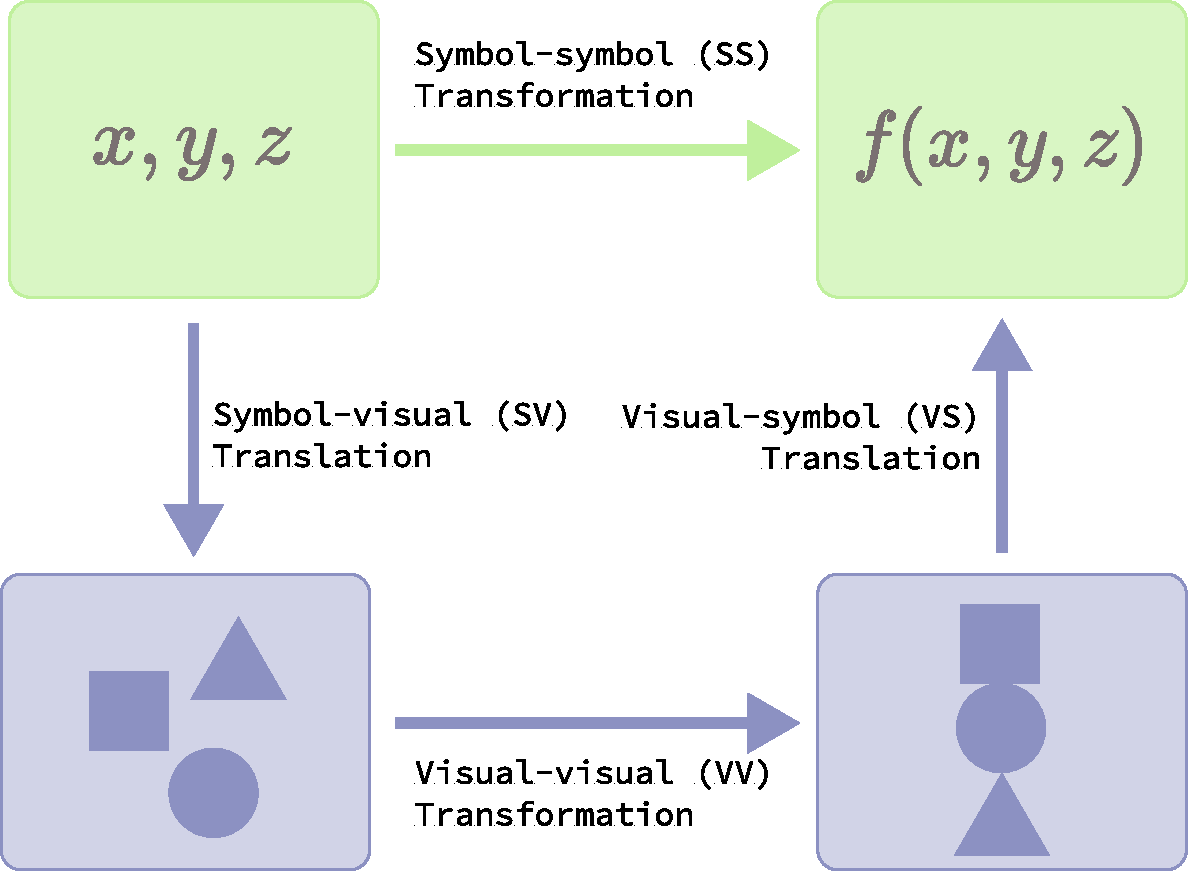
\includegraphics[width=0.45\textwidth]{assets/chapter-1/grounding-rectangle.pdf}
%   \end{center}
% \end{wrapfigure}

% Let me use a diagram to capture this: the \textbf{grounding rectangle} represents two pathways to learning and problem solving: One can perform symbol-to-symbol transformations (SS, or “symbol pushing”) or through an \textcolor[HTML]{8C91C2}{alternative diagrammatic pathway}: a symbol-to-diagram translation (SV), a diagram-to-diagram transformation (VV), and finally a diagram-to-symbol translation (VS).


% Research on expertise development suggests a need for substantial exposure involving repetition in varied contexts or deliberate practice \cite{deliberatePractice} to acquire the perceptual chunks \cite{chunkingModels, perceptualLearningExpertise} that support accurate interpretation and use of visual representations~\cite{Koedinger1990a}. Through enough practice, learning the two paths in the grounding rectangle can produce better, more robust memory \cite{dualCoding}, learning~\cite{multipleReps, multimediaLearning, cotraining}, and future reasoning, both in providing flexibility and in supporting error recovery \cite{groundedAndAbstractReps}.

\chapter{Background and Related Work}
\label{chp:background}

\chapter[Understanding the Diagramming Process]{Understanding the Diagramming Process\footnote{This chapter is adapted from \textit{How Domain Experts Create Conceptual Diagrams and Implications for Tool Design}~\cite{naturalDiagramming}.}}
\label{chp:interviews}

\chapter{Understanding the diagramming process and encoding visual representations}
\label{chp:interviews}

Before diving into the educational context, it's important to understand why creating diagrams is hard in the first place. This chapter discusses an interview study on how domain experts including educators use diagramming tools~\cite{naturalDiagramming}, and briefly shows how this study informs the design of \Penrose, the technical basis for tools presented in this proposal. 

\section{How domain experts create diagrams and implications for tool design}
\label{sec:naturalDiagramming}

Existing diagramming tools stand in tension between: a) General-purpose drawing tools such as Illustrator and Figma that offer simple pen-and-canvas or box-and-arrow metaphors, but are viscous~\cite{cognitiveDimensions}---users must constantly commit to exact positions, sizes, and styling of shapes. b) Dedicated diagramming tools such as Lucidchart and Gliffy that allow rapid changes, but rely heavily on templates, limiting diagrammers to a fixed set of visual representations. This relatively limited support for diagramming in tools is in part because the process of diagramming is poorly understood. For instance, how do diagrammers utilize the strengths and cope with the limitations of their tools? Which tools are chosen for what purposes?  Such a detailed understanding of the process can help design interactive tools to support diagramming.

I conducted interviews with 18 domain experts from a wide variety of disciplines such as math, computer science, architecture, and education. The interviews reveal that diagrammers have diverse interactions with visual representations in both physical sketches and digital tools, including finding, creating, storing, and reusing representations. 

One implication of our results is the opportunity to design tools informed by the processes of diagramming, and practices that domain experts already use, making digital diagramming more intuitive and efficient. Here are four key opportunities for natural~\cite{naturalProgramming} diagramming tools that allow diagrammers to express their ideas visually the same way they think about them:

\begin{itemize} 
    \item \textit{Exploration support}: supporting exploratory behaviors such as undo and backtracking during both abstract-level, breath-first exploration of the design space and low-level refinements of visual details.
    \item \textit{Representation salience}: allowing explicit creation and management of visual representations, \ie, the \emph{mappings} from domain constructs to shapes instead of geometric primitives themselves.
    \item \textit{Live engagement}: providing diagrammers with the sense of agency by designing for liveness and directness of the diagramming experience. 
    \item \textit{Vocabulary correspondence}: enabling diagrammers to interact with their diagrams using vocabularies that is conventional in their domain.
\end{itemize}


\chapter[\Penrose: From Notations to Beautiful Diagrams]{\Penrose: From Notations to Beautiful Diagrams\footnote{
This chapter is adapted from \textit{\Penrose: From Mathematical Notation to Beautiful Diagrams} \cite{penrose}
}}
\label{chp:penrose}
\begin{figure}[h]
  \centering
\begin{minipage}{120pt}
   \fontsize{7pt}{8pt}\selectfont
   \texttt{\textbf{Point} p, q, r, s} \\
   \texttt{\textbf{Segment} a := \{p, q\}} \\
   \texttt{\textbf{Segment} b := \{p, r\}} \\
   \texttt{\textbf{Point} m := \textbf{Midpoint}(a)} \\
   \texttt{\textbf{Angle} theta := $\angle$(q, p, r)} \\
   \texttt{\textbf{Triangle} t := \{p, r, s\}} \\
   \texttt{\textbf{Ray} w := \textbf{Bisector}(theta)} \\
   \texttt{\textbf{Ray} h := \textbf{PerpendicularBisector}(a)} \\
\end{minipage}\hfill
% \hspace{0pt}%
\begin{minipage}{340pt}
   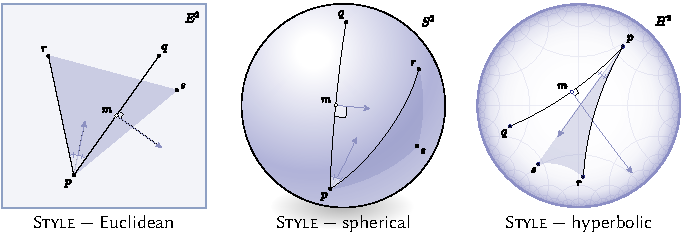
\includegraphics{assets/penrose/teaser.pdf}
\end{minipage}
   \caption{\Penrose{} is a framework for specifying how mathematical statements should be interpreted as visual diagrams.  A clean separation between abstract mathematical objects and their visual representation provides new capabilities beyond existing code- or GUI-based tools.  Here, for instance, the same set of statements (left) is given three different visual interpretations (right), via Euclidean, spherical, and hyperbolic geometry.
   \label{fig:penrose-teaser}
   }
\end{figure}

Informed by the results from the interview study (\cref{chp:interviews}), we developed \Penrose, a language-based diagramming platform~\cite{penrose}. The core \Penrose system addresses \textbf{representation salience}: it has first-class support for creating and reusing visual representations. To accomplish this, \Penrose decomposes the concerns of diagramming into two domain-specific languages (DSLs) with distinct purposes: \Substance contains the mathematical content of the diagram. \Style explicitly specifies mappings from mathematical objects to visual icons. In contrast to tools that specify diagrams via direct manipulation or low-level graphics programming, \Penrose{} enables creation and exploration of diagrams that faithfully preserve the underlying mathematical meaning. \cref{sec:Introduction,sec:SystemDesign} explain the overall design goals; \cref{sec:LanguageFramework,sec:LayoutEngine} detail \Penrose{}'s language design and automatic layout engine that powers its runtime. \cref{sec:ExamplesandEvaluation} demonstrates the effectiveness and generality of the system by showing how it can be used to illustrate a diverse set of concepts from mathematics and computer graphics.

\section{Introduction}
\label{sec:Introduction}

A central goal of \Penrose{} is to lower the barrier to turning mathematical ideas into effective, high-quality visual diagrams.  In the same way that \TeX\ and \LaTeX\ have democratized mathematical writing by algorithmically codifying best practices of professional typesetters~\cite{Beeton:2016:CMT}, \Penrose{} aims to codify best practices of mathematical illustrators into a format that is reusable and broadly accessible.

Our approach is rooted in the natural separation in mathematics between abstract definitions and concrete representations. In particular, the \Penrose{} system is centered around the specification of a \emph{mapping} from mathematical objects to visual icons (\cref{sec:SystemDesign}).  Such mappings are expressed via domain-specific languages (DSLs) that reflect familiar mathematical notation and can be applied to obtain new capabilities that are difficult to achieve using existing tools (\cref{sec:related-systems}).  A key distinction is that \Penrose{} programs encode a \emph{family} of possible visualizations, rather than one specific diagram.  Hence, effort put into diagramming can easily be reused, modified, and generalized.  This approach has several broad-reaching benefits:

\begin{itemize}
   \item \textbf{Accessibility.} Novice users can generate diagrams by simply typing mathematical statements in familiar notation, leveraging the efforts of more expert package developers.
   \item \textbf{Separation of content and presentation.} The ability to easily swap out different visual representations helps deepen understanding by illustrating the same mathematical concepts from many different visual perspectives.
   \item \textbf{Evolution of collections.} Existing collections of diagrams can easily be improved and modified to meet the needs of a target platform, \eg{} desktop vs. mobile, different printing processes, or different language localizations.
   \item \textbf{Large-scale generation.} It becomes easy to generate large collections of illustrations to explore an idea, or to accompany, say, randomly-generated homework exercises.
   %\item \textbf{Interactive exploration.} Diagrams preserve a given set of relationships \emph{by construction}, and can hence be manipulated without violating the intended mathematical meaning.
\end{itemize}

Beyond describing the implementation of \Penrose{}, the purpose of this chapter is to explore the general challenge of designing systems for diagram generation. We hence start with a discussion of goals and trade-offs that inform our system design (\cref{sec:SystemDesign}). Readers may also find it helpful to periodically refer to the more detailed but purely descriptive account of the system given in \cref{sec:LanguageFramework} and \cref{sec:LayoutEngine}.

\section{System Design}
\label{sec:SystemDesign}


Our aim is to build a system for converting abstract mathematical ideas into visual diagrams.  Choices about system design are guided by several specific goals, many of which are supported by interviews presented in \cref{chp:interviews}:
\begin{enumerate}
   \item Mathematical objects should be expressed in a familiar way.\refstepcounter{goalcounter}\label{gol:FamiliarNotation} % Later we say: what could be better than mathematical notation?
   \item The system should not be limited to a fixed set of domains.\refstepcounter{goalcounter}\label{gol:NoFixedDomains} % Many new domains in mathematics will undoubtedly be discovered in the coming years.
   \item It should be possible to apply many different visualizations to the same mathematical content.\refstepcounter{goalcounter}\label{gol:ManyViz} % Because there are often many different ways to visually represent a given mathematical idea, i
   \item There should be no inherent limit to visual sophistication.\refstepcounter{goalcounter}\label{gol:sophistication}  % The system should allow use of ``best in class'' graphical algorithms to generate diagrams.
   \item It should be fast enough to facilitate an iterative workflow.\refstepcounter{goalcounter}\label{gol:FastEnough}  % Overall we aim for performance commensurate with other document or presentation creation tools.
   \item Effort spent on diagramming should be generalizable and reusable.\refstepcounter{goalcounter}\label{gol:Reuse}
\end{enumerate}

To achieve these goals, we take inspiration from the way diagrams are often drawn by hand.  In many domains of mathematics, each type of object is informally associated with a standard \emph{visual icon}.  For instance, points are small dots, vectors are little arrows, \etc{}  To produce a diagram, symbols are systematically translated into icons; a diagrammer then works to arrange these icons on the page in a coherent way.  We formalize this process so that diagrams can be generated computationally, rather than by hand.  Specifically,

\begin{figure}[t]
   \centering
   \begin{minipage}[c]{.35\linewidth}
       \caption{High-level pipeline: a compiler translates mathematical statements and a chosen visual representation into a constrained optimization problem.  This problem is then solved numerically to produce one or more diagrams.\label{fig:HighLevelPipeline}}
   \end{minipage}\hfill
   \begin{minipage}[c]{.60\linewidth}
       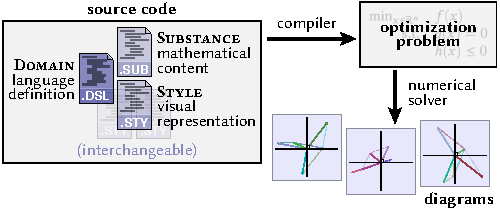
\includegraphics[width=\linewidth]{assets/penrose/HighLevelPipeline.pdf}
   \end{minipage}\hfill
   \vspace{-\baselineskip}
\end{figure}


\vspace{.5\baselineskip}\begin{mdframed}
The two organizing principles of \Penrose{} are:
   \begin{enumerate}[label=(\roman*)]
      \item to \textbf{specify} diagrams via a mapping from mathematical objects to visual icons, and
      \item to \textbf{synthesize} diagrams by solving an associated constrained optimization problem.
   \end{enumerate}
\end{mdframed}\vspace{.5\baselineskip}


Just as the occupant of Searle's ``Chinese room''---who, without understanding Chinese, follows instructions to manipulate symbols and appear as if they understand the language--- does not actually understand a foreign language~\cite{Cole:2014:CRA}, a system designed this way need not perform deep reasoning about mathematics. It simply does a translation.  We hence do not expect our system to solve all challenges of diagramming. Users are still responsible for, say,
\begin{itemize}
   \item choosing meaningful notation for a mathematical domain,
   \item inventing a useful visual representation of that domain, and
   \item ensuring that diagrams correctly communicate meaning.
\end{itemize}

\setlength{\columnsep}{1em}
\setlength{\intextsep}{0em}
\begin{wrapfigure}{r}{0.4\linewidth}
% \begin{figure}
% {128pt}
\begin{minipage}{60pt}
\begin{lstlisting}[language=Sub-ST,escapechar=@,numbers=none]
Set A, B
Point p
A $\subset$ B
p $\in$ A
p $\notin$ B
\end{lstlisting}
\end{minipage}\hfill
\begin{minipage}{120pt}
  \centering
  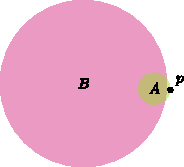
\includegraphics[width=\linewidth]{assets/penrose/sets-inconsistent.pdf}
\end{minipage}
   \vspace{-.5\baselineskip}\caption{An optimization-based approach has myriad benefits.  Here a logically inconsistent program fails gracefully, providing visual intuition for \emph{why} the given statements cannot hold.\label{fig:sets-inconsistent}}
\end{wrapfigure}
% \end{figure}

Likewise, a system cannot be expected to solve hard computational or mathematical problems (\eg the halting problem or Fermat's last theorem) in order to construct diagrams.  Yet despite this shallow level of reasoning, \Penrose{} is able to generate quite sophisticated diagrams.  In fact, even in the absence of such reasoning, na\"{i}ve visualization often provides useful observations (\cref{fig:sets-inconsistent}).

The resulting system effectively models diagram generation as a compilation process, where the compilation target is a constrained optimization problem rather than (say) a binary executable or a static image.  Once compiled, this problem can be used and \emph{reused} to generate visual diagrams; \cref{fig:HighLevelPipeline} illustrates the high-level system flow.  From a programming language point of view, a mapping expressed in this framework defines an \emph{executable visual semantics}. That is, it gives a specific, visual, and computable interpretation to what were previously just abstract logical relationships.

\subsection{Language-Based Specification}
\label{sec:LanguageBasedSpecification}

\begin{figure}
   \centering
   %\includegraphics{assets/penroseRetargeting.pdf}
   \begin{minipage}[c]{.30\linewidth}
   \caption{By specifying diagrams in terms of abstract relationships rather than explicit graphical directives, they are easily adapted to a wide variety of use cases.  Here we use identical \Penrose{} code to generate ray tracing diagrams for several targets (\cref{sec:RayTracing}). The \Style{} program for this domain makes use of a plugin that expands the regular expression for light paths based on the canvas size, \ie small canvases get fewer bounces in the light path. Though the arrangement and number of objects changes in each example, the meaning remains the same.\label{fig:Retargeting}}
  \end{minipage}\hfill
  \begin{minipage}[c]{.6\linewidth}
   \begin{overpic}{assets/penrose/Retargeting.pdf}
      \put(60,15) {\parbox{2in}{
         \texttt{\textbf{PathType} t} \\
         \texttt{\textbf{HasForm}(t,"L(D|S)S*E")} \\
         \texttt{\textbf{Path} p := \textbf{Sample}(t)}
      }}
   \end{overpic}
   \end{minipage}
\end{figure}


A major decision in \Penrose{} is to use programming languages to specify both mathematical objects and their visual representation.  Graphical (\eg sketch-based) specification would demand that users already know how to visualize abstract ideas, and it ties mathematical content to one specific visual representation, which conflicts with \ref{gol:ManyViz}.  A language-based specification provides the level of abstraction needed to separate content from visualization. This technique supports \ref{gol:FamiliarNotation}, since language is the most common means by which mathematical ideas are expressed.  From a system design point of view, a language-based encoding provides a unified representation for identifying and transforming mathematical objects throughout the pipeline.  Moreover, a language-based interface makes it easy for \Penrose{} to provide a \emph{platform} on which other diagramming tools can be built (as in \cref{sec:DevelopmentEnvironment} or \cref{sec:LargeScaleDiagramGeneration}).  One trade-off is that a language-based approach requires users to express themselves in formal mathematical or computational language, making it more difficult for (say) visual artists and designers to contribute new representations.

\begin{figure}[b]
% \vspace{-\baselineskip}
  \begin{minipage}[c]{.35\linewidth}
    \caption{Most \Penrose{} users need only use the \Substance{} language, but can benefit from packages written by more expert \Domain{} and \Style{} programmers. This is similar to the \TeX ecosystem, where most users only write documents, but benefit from expert-authored packages.\label{fig:NoviceExpertUsers}}
  \end{minipage}\hfill
  \begin{minipage}[c]{.55\linewidth}
     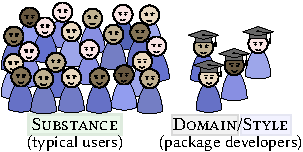
\includegraphics[scale=1.5]{assets/penrose/NoviceExpertUsers.pdf}
  \end{minipage}\hfill
\end{figure}

A secondary decision is to split specification of mathematical content and visualization across two domain-specific languages: \Substance{} and \Style{}.  A good analogy is the relationship between HTML \cite{BernersLee:1995:HML}, which specifies content, and CSS~\cite{Lie:2005:CSS}, which describes how it is rendered.  A schema called \Domain{} (analogous to XML or JSON schemas) defines the mathematical domain of interest, supporting \ref{gol:NoFixedDomains}. A detailed walkthrough of an example trio of \Domain{}, \Substance{}, and \Style{} is included in \cref{app:penrose-trio-walkthrough}.  In line with \ref{gol:ManyViz}, this division allows the same styles to be reused for different content, and likewise, the same content to be displayed in many different styles.  Our goal is for this division to support an ecosystem where novice users can benefit from packages written by more experienced developers (\cref{fig:NoviceExpertUsers}).  Finally, as in mathematics, the ability to adopt user-defined, domain-specific notation (\cref{sec:MathematicalDomain}) enables efficient expression of complex relationships in a way that is both concise and easy to understand~\cite{Kosar:2012:PCD}.  Encoding ideas directly in the idiom of a problem domain often results in better program comprehension than (say) a sequence of library calls in a general-purpose language~\cite{van_deursen_domain-specific_2000}.  We discuss the scope and limitations of our languages in~\cref{sec:DiscussionandFutureWork}.





\subsubsection{Mathematical Domain (\Domain{})}
\label{sec:MathematicalDomain}

\begin{figure}
   \begin{minipage}[c]{.35\columnwidth}
      \vspace{5\baselineskip}\caption{One benefit of a unified framework is that different domains are easily combined.  Here, two existing packages (for meshes and set theory) were combined to illustrate that a simplicial complex \figloc{(left)} is closed with respect to taking subsets \figloc{(right)}.\label{fig:DomainInterop}}
   \end{minipage}\hfill
   \begin{minipage}[c]{.55\columnwidth}
  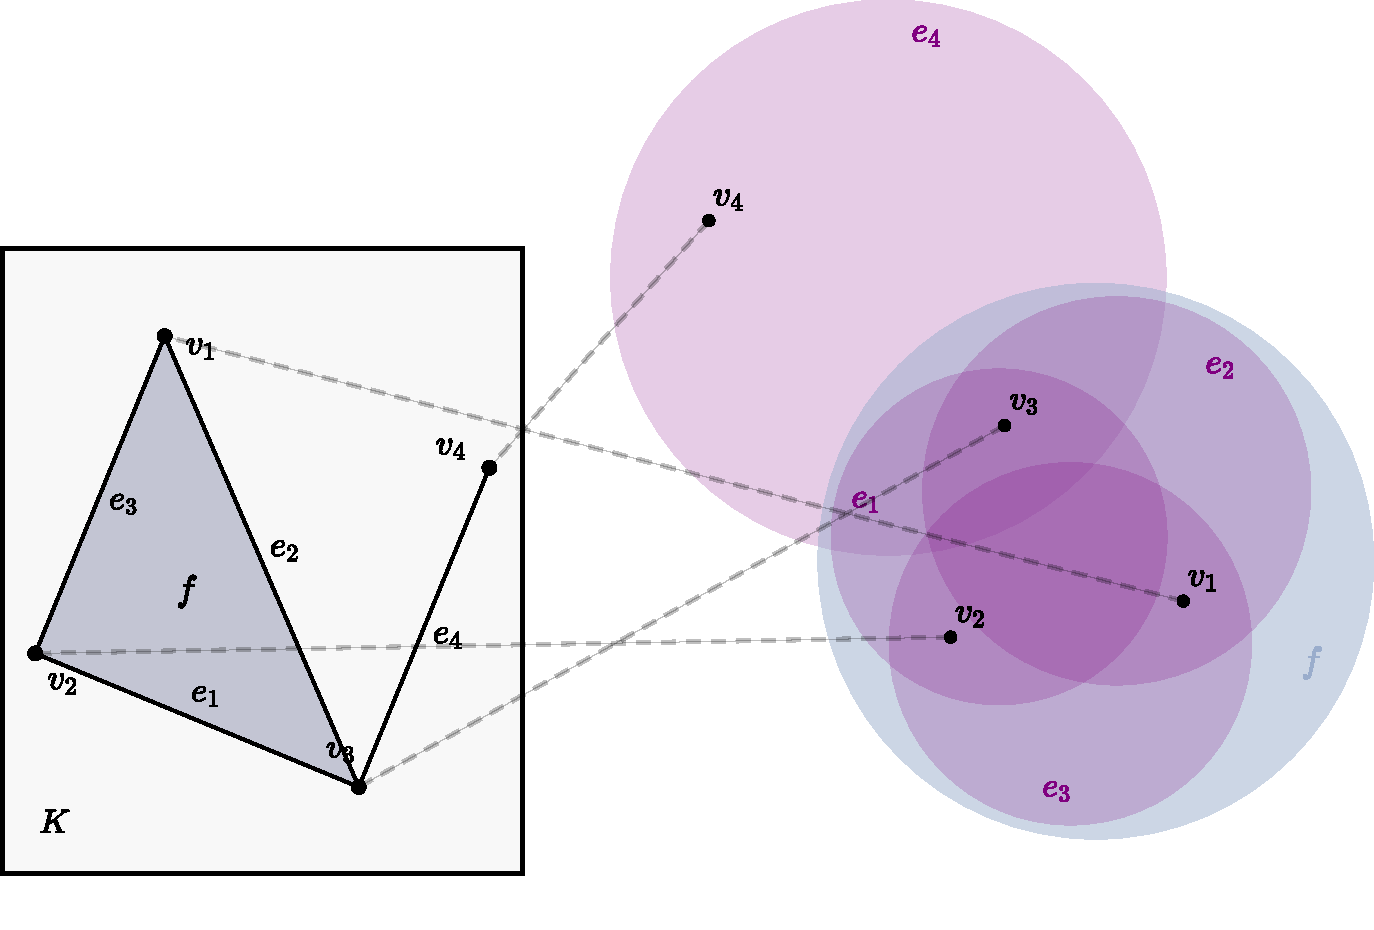
\includegraphics[width=\textwidth]{assets/penrose/domain-interop.pdf}
   \end{minipage}\vspace{-\baselineskip}
\end{figure}

One of our primary goals (\ref{gol:NoFixedDomains}) is to build a unified system for diagramming, rather than to focus on specific domains (as in, say, \emph{GraphViz}~\cite{Graphviz} or \emph{GroupExplorer}~\cite{GroupExplorer}).  A unified design enables objects from different domains to coexist in the same diagram, often by doing little more than concatenating source files (\cref{fig:DomainInterop}).  Moreover, effort put into (say) improving system performance or rendering quality is amortized across many different domains.

Users can work in any area of mathematics by writing so-called \Domain{} schemas (\cref{sec:TheDomainSchema}) that define DSLs tailored to a given domain.  This design also empowers users to adopt their own notation and conventions for modeling the domain.  Use of domain- and user-specific notation reflects common practice in mathematical writing, where the meaning of a symbol is frequently overloaded depending on context.  Importantly, a \Domain{} schema is purely abstract: it does not define an internal representation for objects, nor does it give definitions to functions or predicates.  This level of abstraction is crucial for \ref{gol:ManyViz}, since it allows multiple visual representations to later be applied to objects from the same domain.

\subsubsection{Mathematical Content (\Substance{})}
\label{sec:MathematicalContent}

% P1: What should this language look like?  Why does our design look the way it does?  Use alternatives to motivate this.
To define the content of a diagram, one must be able to specify (i) the objects in the diagram, and (ii) relationships among these objects.  In line with \ref{gol:FamiliarNotation}, \Substance{} uses concise assertions that resemble standard mathematical prose (see for example \cref{fig:MathProse}).  Formally, it can model any domain expressible in a compositional language of types, functions, and predicates, which are the basic constructs found in conventional mathematical notation~\cite{ganesalingam2013language}.  Just as definitions are typically immutable in mathematics, \Substance{} draws inspiration from strongly typed functional languages (such as \emph{ML}~\cite{Milner:1997:DSM}) where objects are stateless.  This choice also simplifies system implementation, since the compiler can assume fixed definitions.  % P2: No data, just viz!
A conscious design decision, in line with \ref{gol:ManyViz}, is to exclude all graphical data (coordinates, sizes, colors, \etc{}) from \Substance{}---since its sole purpose is to specify \emph{abstract relationships} rather than \emph{quantitative data}.  All such data is instead specified in \Style{} or determined via optimization.  This division relieves users from the burden of tedious and repetitive graphics programming, which can instead be factored out into reusable \Style{} code.

% P3: What are possible alternatives?
Existing languages would be difficult to use in place of \Substance{} since they lack the semantics needed to encode complex logical relationships and do not provide language-level extensibility.  For instance, \TeX{} \cite{Beeton:2016:CMT} and \emph{MathML} \cite{Miner:2005:IMM} markup provide only enough information to translate plain text into mathematical glyphs; computer algebra systems like \emph{Mathematica} and \emph{Maple} have limited type systems or provide only a small set of fixed predicates (\eg asserting that a number is real).  Conversely, the much richer languages used by automated theorem provers and proof assistants (such as \emph{Coq}~\cite{Bertot:2013:ITP} and \emph{Lean}~\cite{deMoura:2015:LTP}) are overkill for simply specifying diagrams. A custom language provides simple, familiar syntax and clear error messages.  We do however adopt some ideas from \emph{Coq}, such as the ability to customize syntactic sugar (\cref{sec:TheDomainSchema}).

\begin{figure}[t]
   \centering
   \hspace{-.5em}\begin{minipage}{120pt}
      \small\emph{For any vector space \(X\), let \(u, v \in X\) be orthogonal vectors of equal length, and let \(w = u+v\).  Then \(u\) and \(w\) make a \(45^\circ\) angle.}
   \end{minipage}
   \hspace{-.5em}\begin{minipage}{160pt}
  \begin{lstlisting}[language=Sub-LA,escapechar=@,numbers=none]
     VectorSpace X
     Vector u, v $\in$ X
     Orthogonal(u, v)
     EqualLength(u, v)
     Vector w $\in$ X
     w := u + v\end{lstlisting}
   \end{minipage}
   \hspace{.5em}\begin{minipage}{120pt}
      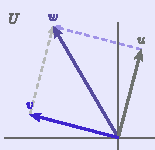
\includegraphics[width=\linewidth]{assets/penrose/MathProse.pdf}
   \end{minipage}
   \caption{Extensibility enables users to adopt conventions and notation \figloc{(center)} that reflect the way they naturally write mathematical prose \figloc{(left)}.  Here, the resulting diagram \figloc{(right)} plays the role of the concluding statement.\label{fig:MathProse}}
\end{figure}


\subsubsection{Mathematical Visualization (\Style{})}
\label{sec:MathematicalVisualization}

% The \Style{} language is used to encode a generic mapping from mathematical objects or relationships that might appear in a \Substance{} program to their visual representation.

% P1: WHAT do we specify? Constraints and objectives
The meaning of a diagram is largely conveyed by relative relationships rather than absolute coordinates.  Moreover, diagrams are often underconstrained: relationships needed to convey the intended meaning determine a \emph{family} of possible solutions, rather than a single unique diagram.  \Style{} hence adopts a constraint-based approach to graphical specification in the spirit of \emph{Sketchpad} \cite{sketchpad}: diagrams are built up from constraints and objectives (\cref{sec:ConstraintsAndObjectives}), then unspecified quantities are solved for via numerical optimization (\cref{sec:LayoutEngine}).  Though procedural definitions can still be used, the programmer need not provide absolute coordinates (as in imperative languages like \emph{PostScript} or \emph{OpenGL}).  Though an implicit specification can make output hard to predict, part of the allure of \Penrose{} is the potential to find interesting or surprising examples.  Moreover, the approach yields more concise code; for instance, \Style{} programs are much shorter than the SVG files they produce.

% P3 What are the alternatives? APIs, visual programming
An alternative design might be to use an application programming interface (API), though historically APIs have been eschewed for specification languages for good reason. Language provides far more concise expression of complex relationships---imagine styling an entire website via the DOM API's \texttt{getElementById()} and \texttt{setStyle()} methods, versus a few short lines of CSS. Visual programming languages (like \emph{LabView}~\cite{Elliott:2007:NIL} or \emph{Grasshopper}~\cite{McNeel:2010:GGM}) might suffice for basic specifications (\eg vectors should be drawn as arrows), but don't scale to more complex concepts that are easily expressed via language~\cite{Burnett:1995:SUV}.

A key design challenge is identifying objects that appear in a \Substance{} program.  Objects in a given mathematical universe are distinguished not only by their type, but also by their relationships to other objects.  A widely-used mechanism for specifying such relationships is through CSS-like \emph{selectors}. \Style{} adopts a similar mechanism that performs pattern matching on the types, functions, and predicates appearing in a \Domain{} schema (\cref{sec:Selectors}).


\subsection{Optimization-Based Synthesis}
\label{sec:OptimizationBasedSynthesis}

The second major design decision in \Penrose{} is to use constrained optimization to synthesize diagrams satisfying a given specification (\cref{sec:LayoutEngine}).  This approach is again inspired by how people often draw diagrams by hand (\eg using GUI-based tools): visual icons are placed on a canvas and iteratively adjusted until no further improvements can be made.  In difficult scenarios, a diagrammer may try several global arrangements before refining the final design, though typically no more than a few.  Automating this process makes it easy to perform layout tasks that would be tedious by hand (\cref{fig:sets-color-opt}).

\begin{figure}[h]
  \centering
  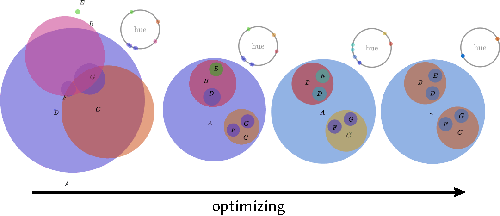
\includegraphics[scale=1.5]{assets/penrose/sets-color-opt.pdf}
  \caption{An optimization-based approach makes it possible to jointly optimize visual attributes that are difficult to coordinate by hand.  Here for instance we optimize color contrast according to the spatial proximity of adjacent disks \figloc{(left to right)}, ultimately discovering a two-color solution \figloc{(far right)}.  The system can also be used to debug the optimization process itself---in this case by drawing the hue of each disk as a dot on a color wheel.\label{fig:sets-color-opt}}
\end{figure}

There are good reasons to believe that an optimization-based approach can scale to very complex diagrams.  First, attractive diagrams need not be optimal in a \emph{global} sense---they should simply not permit obvious \emph{local} improvements, such as text that could easily be moved closer to the item it labels. In fact, disparate local minima can provide useful examples that help build intuition (\cref{fig:enumerate-subsets}).  Second, even sophisticated diagrams have surprisingly few degrees of freedom in comparison to many modern optimization problems (\eg tens or hundreds, versus thousands or millions).  Finally, strategies employed by expert diagrammers can be applied to manage complexity, such as independently optimizing small components of a diagram (akin to nonlinear Gauss-Seidel), rather than optimizing all degrees of freedom simultaneously.

In line with \ref{gol:NoFixedDomains} and \ref{gol:ManyViz}, an optimization-based approach can be applied generically and automatically for any user-defined domain and visual representation, without requiring programmers to think about the details of the layout process.  In our system, the optimization problem is defined using common-sense keywords (\cref{sec:ConstraintsAndObjectives}) in \Style\ and chaining together basic operations (\eg arithmetic).  Since the diagram specification is divorced from the details of the solver, optimization strategies can be changed and improved in future versions of the system while preserving compatibility with existing code.  The main cost of an optimization-based approach is that it puts demands on system design ``upstream'': all expressions used to define a visual style must be differentiable. As discussed in \cref{sec:Solver}, these requirements are largely satisfied via standard techniques (\eg{} by using \textit{automatic differentiation}).

\begin{figure}[t]
   \begin{minipage}[c]{.5\linewidth}
   \includegraphics{assets/penrose/enumeration.pdf}
   \end{minipage}\hfill
   \begin{minipage}[c]{.4\linewidth}
   \caption{A language-based design makes it easy to build tools on top of \Penrose{} that provide additional power. Here we use standard techniques from program synthesis (\cref{sec:LargeScaleDiagramGeneration}) to automatically enumerate how the given relationships can be realized.  Generating such examples helps to see important corner cases that might be missed when drawing diagrams by hand (where perhaps the top-left diagram most easily comes to mind).\label{fig:enumerate-subsets}}
   \end{minipage}
\end{figure}

% , and each graphical primitive must support efficient geometric queries (\eg bounding box evaluation and closest point queries). 

In general, diagram optimization is a challenging problem in its own right, which we of course do not aim to solve conclusively in this chapter.  Currently, we just use a generic constrained descent solver (\cref{sec:Solver}).  However, we have been pleased to find that this simple approach handles a wide variety of examples from different domains without requiring domain-specific strategies.


\subsection{Plugins}
\label{sec:PlugInDesign}

% TODO: Review the rewritten plugin sections

% Design decision 1: Have a plugin system for integrating external code
% Why? Further extensibility. Can't be a closed system. Lots of existing mathematical code that just needs the right interface, e.g. specialized mesh processing code.

% Decision 2. The plugin interface. A plugin receives Substance code and Style floats; outputs Substance code only (appended to file) and Style constants.
% Why? Keep it abstract, so you can use Penrose. augment set of abstract objects; provide basic information about their layout, but doesn't directly style them. Limit the power of a plugin: simplicity and modularity. 

% Decision 3. (Goes in "system" section) How to use a plugin: (Substance code JSON, Style constants as floats) -> (append Substance code as text file; output JSON for style)
% Why? JSON, floats, text files are all easy and portable, rather than calling an "API machine". Plugin can be written in any languge as long as it satisfies this inteface.

The final design decision in \Penrose\ is to provide system-level extensibility via a \textit{plugin} interface for calling external code in \Substance\ and \Style. Providing a plugin system is essential to enable users to integrate external code that is specialized to solve particular logical or graphical challenges. In fact, such interfaces for integrating external code are already provided by many systems (\eg \TeX, \emph{Adobe Illustrator}, and TikZ's plugin system for graph layout algorithms~\cite{Graphviz}). The interface for \Penrose\ plugins is designed to define a clear and simple boundary between the \Penrose\ system and the plugin while enabling each component to focus on its strengths. A plugin can analyze and augment the set of abstract objects defined in \Substance{}, as well as analyze and augment the numerical information in \Style. This simple interface allows plugins to be written in any language (or repurposed from other systems) and operate independently from the implementation details of \Penrose. However, a plugin cannot change an existing \Substance\ or \Style\ program or directly generate static graphical content, since such plugins would abandon the benefits that \Penrose{} provides, such as the ability to re-style content and avoid use of absolute coordinates. \cref{fig:Retargeting} illustrates how a simple plugin can make use of \Substance\ and \Style\ information to create ``responsive'' diagrams.

% Since the \Penrose\ system focuses on diagram specification and synthesis, it does not natively perform sophisticated logical reasoning for \Substance\ programs. Additionally, we want to provide a way for users to avoid reinventing the wheel when it comes to graphical layout in \Style.


\section{Language Framework}
\label{sec:LanguageFramework}

The \Penrose{} language framework comprises three languages that play different roles:

\begin{itemize}
   \item A \inlineDSL{\Domain{} schema} declares the objects, relationships, and notation available in a mathematical domain.
   \item A \inlineSUB{\Substance{} program} makes specific mathematical assertions within some domain.
   \item A \inlineSTY{\Style{} program} defines a generic mapping from mathematical statements in some domain to a visual representation.
\end{itemize}

A \emph{package} consisting of a \(\Domain{}\), and one or more compatible \(\Style{}\) programs, can be used to illustrate \Substance{} programs from a given domain (\cref{fig:HighLevelPipeline}).  Though some starter packages are provided for the examples discussed in~\cref{sec:ExamplesandEvaluation}, the real power of \Style{} and \Domain{} is that they enable \Penrose\ to be easily extended.  In this section we illustrate these languages via the running example of a linear algebra package (Figures~\ref{fig:domain_linalg} through \ref{fig:style_linalg}).  
% Formal grammars for the three languages are given in supplemental material.



\subsection{The \Domain{} Schema}
\label{sec:TheDomainSchema}

A \Domain{} \emph{schema} describes a domain of mathematics by defining the objects and notation that can be used by associated \Substance{} and \Style{} programs.  A partial example for linear algebra is shown in \cref{fig:domain_linalg}.  The \inlineDSL{\keyword{type}} lines define the available object types, \inlineDSL{\keyword{function}} lines define the domain and codomain for the set of available functions (where \texttt{*} denotes a Cartesian product), and \inlineDSL{\keyword{predicate}} lines define the possible relationships among objects, including unary predicates.  Importantly, a \Domain{} schema is purely abstract: it does not define a specific representation for objects, nor does it define bodies for functions or predicates. For instance, we do not say here that a vector is encoded by a list of coordinates, nor do we write an addition operation on such coordinates.  A concrete visual interpretation of these definitions is given by a \Style{} program (\cref{sec:TheStyleLanguage}).  Types can be given fields via \emph{constructors}. For instance, the line
\[
   \text{\small\texttt{\textbf{constructor} MakeInterval: Real min * Real max -> Interval}}
\]
assigns fields \texttt{min} and \texttt{max} to an \texttt{Interval}, which can be accessed from a \Substance{} or \Style{} program (\eg to assert a relationship between endpoints).  Subtyping via the syntax \texttt{Subtype <: Type} facilitates generic programming.  Finally, \inlineDSL{\keyword{notation}} lines define optional syntactic sugar that can simplify code (\eg in \cref{fig:substance_linalg}).

\begin{figure}
\begin{mdframed}[style=DSLCode]
\begin{lstlisting}[language=Elem,escapechar=@]
type Scalar, VectorSpace, Vector                            -- LinearAlgebra.dsl @\label{lin:linalg_types}@
function add: Vector * Vector -> Vector @\label{lin:linalg_functions_begin}@
function norm: Vector -> Scalar
function scale: Scalar * Vector -> Vector
... @\label{lin:linalg_functions_end}@
predicate In: Vector * VectorSpace @\label{lin:linalg_predicates_begin}@
predicate Unit: Vector
predicate Orthogonal: Vector * Vector
... @\label{lin:linalg_predicates_end}@
notation "v1 + v2" $\sim$ "add(v1,v2)"
notation "|y1|" $\sim$ "norm(y1)"
notation "s * v1" $\sim$ "scale(s,v1)"
notation "Vector v $\in$ V" $\sim$ "Vector a; In(a,U)"
notation "v1 $\perp$ v2" $\sim$ "Orthogonal(v1,v2)"
...
\end{lstlisting}
\end{mdframed}
   \caption{A \Domain{} schema specifies the building blocks available in a given mathematical domain, as well as any associated syntactic sugar.  This schema (abbreviated) enumerates some basic constructs from linear algebra.\label{fig:domain_linalg}}
\end{figure}


\subsection{The \Substance{} Language}
\label{sec:TheSubstanceLanguage}

Each statement in the \Substance\ language either (i) declares an object, (ii) specifies properties of an object, or (iii) specifies relationships among objects within some \Domain{} schema.  As in mathematics, not all attributes need be fully specified. For instance, one can talk about a point without giving it explicit coordinates. Together, these statements describe a \emph{context} that encloses all the mathematical objects and relationships that have been defined.

\begin{figure}
\begin{minipage}[!t]{140pt}
\begin{mdframed}[style=SUBCode]
\begin{lstlisting}[language=Sub-LA,escapechar=@,numbers=none]
VectorSpace X
Vector x1, x2
In(x1, X)
In(x2, X)
Unit(x1)
Orthogonal(x1, x2)
label x1 @$\$$@x_1@$\$$@
label x2 @$\$$@x_2@$\$$@
\end{lstlisting}
\end{mdframed}
\centering (unsugared)
\end{minipage}
\hfill
\begin{minipage}[!t]{150pt}\vspace{-2\baselineskip}
\begin{mdframed}[style=SUBCode]
\begin{lstlisting}[language=Sub-LA,escapechar=@,numbers=none]
VectorSpace X
Vector x1, x2 $\in$ X
Unit(x1)
x1 $\perp$ x2
label x1 @$\$$@x_1@$\$$@
label x2 @$\$$@x_2@$\$$@
\end{lstlisting}
\end{mdframed}
\centering (sugared)
\end{minipage}
\hfill
\begin{minipage}[!t]{150pt}
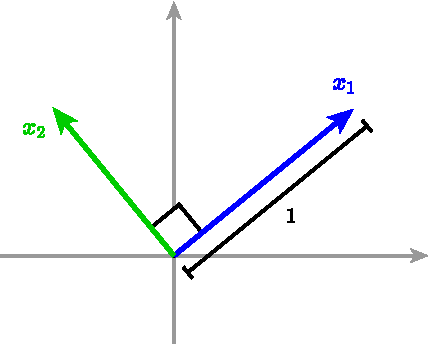
\includegraphics[width=1\columnwidth]{assets/penrose/substance-linalg.pdf}
\end{minipage}
   \caption{When used with the \Style{} defined in \cref{fig:style_linalg}, this \Substance{} code (with or without syntactic sugar) produces the diagram shown at right.\label{fig:substance_linalg}}
\end{figure}

\cref{fig:substance_linalg} shows an example in which \Substance{} code specifies properties and relationships for a pair of vectors.  Importantly, these statements do not induce any kind of numerical evaluation.  For instance, no coordinates are assigned to \texttt{x1} in order to make it unit---in fact, the vector space \texttt{X} does not even have an explicit dimension.  Instead, statements specify persistent and purely symbolic relationships that provide cues for visualization;  specific coordinates and attributes are later determined by the layout engine (\cref{sec:LayoutEngine}). The final lines specify label strings to be used by the \Style{} program, here in \TeX{} notation.  \cref{fig:substance_linalg}, \figloc{center} shows a ``sugared'' version of this program using notation defined in the \Domain{} schema (\cref{fig:domain_linalg}).  Users can write programs either way, depending on the capabilities of their editor (\eg support for Unicode input).


\subsection{The \Style\ language}
\label{sec:TheStyleLanguage}

% TODO Add brief discussion of layering

% TODO Add brief discussion of transforms, "then" keyword

\setlength{\columnsep}{1em}
\setlength{\intextsep}{1em}
\begin{wrapfigure}{l}{200pt}
   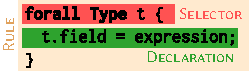
\includegraphics[width=\linewidth]{assets/penrose/StyleNomenclature.pdf}
\end{wrapfigure}
\Style{} specifies how expressions in a \Substance{} program are translated into graphical objects and relationships.  It is a declarative specification language that shares many features with CSS.  The core principle is to sketch out basic \emph{rules} (\eg visual icons for basic types) and then refine these rules via \emph{cascading} (\cref{sec:Cascading}).  Each rule uses a \emph{selector} to pattern match on objects and relationships appearing in \Substance{} code (\cref{sec:Selectors}).  A sequence of \emph{declarations} then specifies a corresponding visualization, \eg by emitting graphical primitives or enforcing constraints.  Each declaration either assigns a \emph{value} to a \emph{field} (\cref{sec:ValuesAndExpressions,sec:Fields}) or specifies a \emph{constraint} or \emph{objective} (\cref{sec:ConstraintsAndObjectives}).  An example is shown in \cref{fig:style_linalg}, which defines part of the style used for the \Substance{} program in \cref{fig:substance_linalg}.  We will use this example to highlight the basic features of the language.  

\begin{figure}[p]
\begin{mdframed}[style=STYCode]
\begin{lstlisting}[language=Sty-LA,escapechar=@]
forall VectorSpace U {                                      -- LinearAlgebra.sty@\label{lin:VectorSpaceRule}@
   U.originX = ? -- to be determined via optimization
   U.originY = ? -- to be determined via optimization
   U.origin = (U.originX, U.originY)
   U.xAxis = Arrow { -- draw an arrow along the x-axis
          startX : U.originX - 1 @\label{lin:VSArrowGeometryBegin}@
          startY : U.originY
          endX   : U.originX + 1
          endY   : U.originY @\label{lin:VSArrowGeometryEnd}@
      thickness  : 1.5 @\label{lin:VectorSpaceConstantsBegin}@
          style  : "solid"
          color  : Colors.lightGray @\label{lin:VectorSpaceConstantsEnd}@
   } -- (similar declarations omitted for the y-axis)
}
forall Vector u, VectorSpace U where In(u, U) { @\label{lin:VectorElementRule}@            
   u.arrow = Arrow { @\label{lin:VectorIsALittleArrow}@
      startX : U.originX @\label{lin:VectorArrowStart}@
      startY : U.originY
        endX : ? @\label{lin:PendingArrowEnd}@
        endY : ?
       color : Colors.mediumBlue
   } @\label{lin:VectorIsALittleArrowEnd}@
   u.text = Text {
      string : u.label -- label from Substance code
       color : u.arrow.color @\label{lin:VectorLabelColor}@ -- use arrow's color
   }
   u.start = (u.arrow.startX, u.arrow.startY)
   u.end = (u.arrow.endX, u.arrow.endY)
   u.vector = minus(u.arrow.end, u.arrow.start) @\label{lin:VectorVector}@
   encourage near(u.text, u.end) @\label{lin:LabelObjective}@
   ensure contained(u.end, U.shape)
}
forall Vector u, Vector v @\label{lin:OrthogonalSelector}@
where Orthogonal(u, v) { @\label{lin:OrthogonalRule}@
   local.perpMark = Curve { @\label{lin:OrthogonalShape}@
        pathData : orientedSquare(u.shape, v.shape, U.origin, const.perpLen)
        strokeWidth : 2.0
        color : Colors.black
        fill : Colors.white
   } @\label{lin:OrthogonalShapeEnd}@
   ensure equals(dot(u.vector, v.vector), 0.0) @\label{lin:OrthogonalConstraint}@
}
... -- (similar rule omitted for Unit)
Vector `x2` @\label{lin:VectorBacktick}@ { override `x2`.shape.color = Colors.green; @\label{lin:OverrideVectorColor}@ }
\end{lstlisting}
\end{mdframed}
   \vspace{-.5\baselineskip}\caption{The \Style{} program defining the visual style used in \cref{fig:substance_linalg}, \figloc{right}. Note that this \Style{} program can be reused for many different \Substance{} programs in the same domain.\label{fig:style_linalg}}
   
\end{figure}

\subsubsection{Selectors}
\label{sec:Selectors}

A selector uses pattern matching to specify which objects will be styled by a rule.  Unlike regular expressions, selectors do not match literal strings of \Substance{} code, but rather objects and relationships in the context defined by this code.  A simple example is a selector that matches every instance of a type, indicated by the \inlineSTY{\keyword{forall}} keyword.  For instance, Line~\ref{lin:VectorSpaceRule} matches all vector spaces.  In subsequent declarations, \inlineSTY{\texttt{U}} refers to the vector space \inlineSUB{\texttt{X}} from the \Substance\ program.  The \inlineSTY{\keyword{where}} keyword restricts matches to objects that satisfy one or more relationships; \eg Line~\ref{lin:OrthogonalRule} matches all pairs of orthogonal vectors.  One can also match by name using backticks; \eg Line~\ref{lin:VectorBacktick} matches only the vector \inlineSUB{\texttt{x2}}.  Selectors could be enriched in the future to allow other statements from first-order logic (such as \(\exists\), disjunctions, and conjunctions).

\subsubsection{Cascading}
\label{sec:Cascading}

A cascading mechanism allows rules to be refined for more specialized objects or relationships.  For example, the selector in Line~\ref{lin:VectorBacktick} matches a specific vector, refining an earlier rule that applies to all vectors.  Rule precedence is determined by order in the \Style{} file, and later rules can refer to any previously defined \emph{field} (\cref{sec:Fields}).  The \inlineSTY{\keyword{override}} keyword (Line~\ref{lin:OverrideVectorColor}) hints that a rule will modify an existing field, otherwise the compiler issues a warning.


\subsubsection{Fields}
\label{sec:Fields}

The visual representation of an object is specified by creating \emph{fields} that are assigned \emph{values} (\cref{sec:ValuesAndExpressions}).  For instance, in Lines \ref{lin:VectorIsALittleArrow}--\ref{lin:VectorIsALittleArrowEnd} a field called \inlineSTY{\texttt{u.arrow}} is created and assigned an expression describing an arrow.  Fields are created on assignment and can have any name not conflicting with a reserved word.  Fields not naturally associated with a single object can also be assigned locally to a rule. For instance, Line~\ref{lin:OrthogonalShape} is used to draw a right angle mark between any pair of orthogonal vectors.  Every object automatically has fields \inlineSTY{\texttt{name}} and \inlineSTY{\texttt{label}} storing its \Substance{} name and label string (\resp), as well as any field created via a constructor (\cref{sec:TheDomainSchema}).


\subsubsection{Properties}
\label{sec:Properties}

\Style{} provides built-in graphical primitives (circle, arrow, \etc{}) with a fixed set of \emph{properties}. Like fields, properties can be assigned values (as in Lines~\ref{lin:OrthogonalShape}--\ref{lin:OrthogonalShapeEnd}). If a value is not assigned, it will be assigned a default value, possibly a \emph{pending value} (\cref{sec:ValuesAndExpressions}).  For example, an arrow might be black by default, whereas the width of a box might be optimized (akin to \emph{flexible space} in \TeX).

% Note that the set of graphical primitives is easily extensible (or indeed, the entire rendering frontend), though we do not currently expose such extensibility at the language level.

\subsubsection{Values and Expressions}
\label{sec:ValuesAndExpressions}

Atomic \emph{values} can be combined to form \emph{expressions}.  For instance, Lines \ref{lin:VectorSpaceConstantsBegin}--\ref{lin:VectorSpaceConstantsEnd} assign values, whereas Lines \ref{lin:VSArrowGeometryBegin}--\ref{lin:VSArrowGeometryEnd} assign composite expressions involving inline computation.  Line~\ref{lin:VectorLabelColor} specifies value via a \emph{path}, \ie, a sequence of expressions separated by \inlineSTY{\texttt{.}} characters; such assignments are made by reference.  Expressions can also access values from plugins (\cref{sec:PlugIns}).  A very important construct is \emph{pending values}, denoted by a \inlineSTY{\texttt{?}} as in Line~\ref{lin:PendingArrowEnd}.  This line specifies that the location of the arrow endpoint is not fixed and will be automatically determined by the solver (\cref{sec:LayoutEngine}).

\subsubsection{Constraints and Objectives}
\label{sec:ConstraintsAndObjectives}

Constraints and objectives describe how pending values should behave.  In particular, the \inlineSTY{\keyword{ensure}} keyword defines a constraint. For instance, Line~\ref{lin:OrthogonalConstraint} specifies that two orthogonal vectors must be drawn at right angles.  The \inlineSTY{\keyword{encourage}} keyword specifies an objective. For instance, Line~\ref{lin:LabelObjective} asks that the label for a vector be placed close to its endpoint. These expressions are all translated into energy functions that make up a numerical optimization problem. It is important to note, therefore, that our solver (\cref{sec:Solver}) may converge without satisfying all constraints.


\section{Layout engine}
\label{sec:LayoutEngine}

\begin{figure}[t]
  \centering
  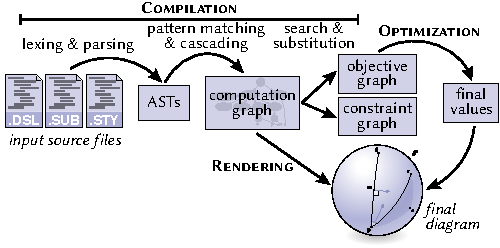
\includegraphics[scale=1.5]{assets/penrose/CompilationPipeline.pdf}
	\caption{Pipeline view of the layout engine.  Rather than a single static image, compilation yields an optimization problem that can be solved and re-solved to produce many diagrams, or (in principle) used in an interactive tool.\label{fig:CompilationPipeline}}
\end{figure}


% (SOURCE [.dsl,.sub,.sty]) ---- "compilation" ----> OPTIMIZATION PROBLEM ---- optimization ----> DIAGRAM
% TODO Turn the ASCII art above into a real diagram that explains (at an appropriate level of granularity) the steps of the Engine

% ENGINE
%  (static compilation)
%    1 check correctness of .dsl
%    2 check correctness of .sub using .dsl
%    3 check correctness of .sty using .dsl
%  (dynamic compilation)
%    4 build dictionary from .sub to .sty
%    5 apply dictionary to transform .sub program into "pre-diagram" + initial guess for unknown state
%       5a Fill in some unknown attributes deterministically (e.g., using defaults or random samples)
%    6 build optimization problem that solves for unknowns in pre-diagram
%  (optimization)
%    7 solve optimization problem
%    8 render the diagram

The layout engine translates \Penrose{} code into images (\cref{fig:CompilationPipeline}).  There are two main stages: a compiler (\cref{sec:Compiler}) translates code into an optimization problem that describes possible diagrams, then a solver (\cref{sec:Solver}) produces solutions to this problem. These values are used to render the final diagram (\cref{sec:Rendering}). For simplicity, the goal is to automatically produce one static diagram, but the same pipeline could be extended to support capabilities like interaction.

% These stages of diagram generation are exposed in a standard Application Programming Interface (API).

\subsection{Compiler}
\label{sec:Compiler}

The input to the compiler is a triple of files: a \Domain{} schema with \Substance{} and \Style{} programs.  The output is a constrained optimization problem, expressed as a computational graph.

\subsubsection{Parsing and Type Checking}
\label{sec:ParsingandTypeChecking}

We parse each of the input files into abstract syntax trees (ASTs), applying static typechecking to ensure that types are well-formed and variables are well-typed.  We first typecheck the \Domain{} program since it defines the valid types for the \Substance{} and \Style{} programs, then use these types to check the \Substance{} program and the selectors in the \Style{} code.
% Our implementation uses a \emph{parser combinator} approach~\cite{Swierstra:2001:CPF}.

\subsubsection{Computational Graph}
\label{sec:ComputationalGraph}

The ASTs are combined to define a \emph{computational graph} that encodes operations that define the final diagram (\cref{fig:build_computation_graph}).  To build this graph, we apply a standard pattern matching and cascading procedure: iterate over rules in the \Style{} program, find tuples of \Substance{} variables that match the selector pattern, then modify the graph according to the declarations within the matched rule.  For example, when the first selector \inlineSTY{\texttt{\textbf{VectorSpace} U}} from \cref{fig:style_linalg} matches the variable \inlineSUB{\texttt{X}} from \cref{fig:substance_linalg}, we add nodes to the graph that encode the axes of this vector space.  In general, declarations could also remove nodes from the graph or connect previously added nodes.  Once this transformation is complete, we have replaced all abstract mathematical descriptions with concrete graphical representatives.  All that remains is to determine pending values (\ie{} those marked by a \inlineSTY{\texttt{?}}) and those values that depend on them, which will be done by the solver.

% Compiler output example: \texttt{https://gist.github.com/hypotext/7895b8e7e1abbe62f5abe84efbc036d6} 

\subsubsection{Optimization Graphs}
\label{sec:OptimizationGraphs}

\begin{figure}
   \begin{minipage}[c]{.4\linewidth}
      \vspace{-\baselineskip}\caption{Applying the mapping defined by \Style{} code to a \Substance{} program yields a graph that describes how to draw the diagram---here, for part of \cref{fig:substance_linalg}.  Some values are known (in blue), whereas others (in orange) depend on unknowns that must be determined via optimization.\label{fig:build_computation_graph}}
   \end{minipage}\hfill
   \begin{minipage}[c]{.5\linewidth}
   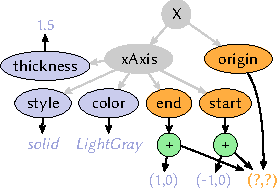
\includegraphics[scale=1.5]{assets/penrose/build_computation_graph.pdf}
   \end{minipage}
\end{figure}

\begin{figure}[t]
\centering
   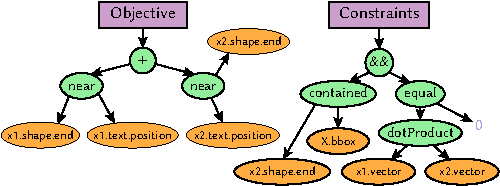
\includegraphics[scale=1.5]{assets/penrose/optimization_computation_graph.pdf}
   \caption{The computation graph is further expanded to produce graphs representing the objective and constraint space for our optimization problem. From there, we can use automatic differentiation to obtain derivatives.  This figure depicts part of the optimization graph for \cref{fig:substance_linalg}.\label{fig:optimization_computation_graph}}
 \end{figure}
 % \setlength{\belowcaptionskip}{-30pt}

 
 To encode the optimization problem, we collect terms from the computational graph into an objective and constraint graph (\cref{fig:optimization_computation_graph}). Each \inlineSTY{\keyword{ensure}} and \inlineSTY{\keyword{encourage}} statement is then replaced by the corresponding mathematical expression.  For instance, \inlineSTY{\texttt{\textbf{ensure} equal(x,y)}} is translated into the constraint \(x-y=0\), which the solver seeks to enforce exactly, whereas \inlineSTY{\texttt{\textbf{encourage} equal(x,y)}} becomes the objective \((x-y)^2\), which the solver seeks to minimize as much as possible.  The overall constraint set is the intersection of all constraints, and the overall objective is a sum of objective terms. Currently \Penrose{} provides a fixed set of constraints and objectives, though it would be straightforward to extend \Style{} to allow user-defined inline expressions.

% TODO Show computational graph for linear algebra example

\subsection{Solver}
\label{sec:Solver}

The optimization graphs produced by the compiler describe an optimization problem in standard form, \ie minimization of an objective function subject to equality and inequality constraints~\cite[Section 4.1]{convexOptimization}.  Such problems may be solved with many standard methods. We currently use an \emph{exterior point method}~\cite{hiroshi_primal-dual_2010} that starts with an infeasible point and pushes it toward a feasible configuration via progressively stiffer penalty functions---mirroring a process often used by hand (\cref{sec:OptimizationBasedSynthesis}). Specifically, \Penrose encodes constraints as nonnegative penalty functions \(\mathcal{P}_1, \ldots, \mathcal{P}_l: \mathbb{R}^m \to \mathbb{R}_{\geq 0}\) each of which equal $0$ if and only if the constraint is satisfied. Objectives are energy terms  \(\mathcal{E}_1, \ldots, \mathcal{E}_k\). Overall, the \Penrose layout engine solves an optimization problem:%
\begin{equation}
   \label{eq:MainProblem}
       \min_{\vec p \in \mathbb{R}^m} \sum_{i=1}^k \mathcal{E}_i(\vec p)  \quad  \text{s.t.} \quad \sum_{i=1}^l \mathcal{P}_i(\vec p) = 0.
\end{equation}%
The exterior point method~\citep{hiroshi_primal-dual_2010} to pose this problem as a sequence of unconstrained optimization problems, where constraints are iteratively stiffened over layout steps: 
\begin{equation}
   \label{eq:ExteriorPointProblem}
   \min_{\vec p \in \mathbb{R}^m} \sum_{i=1}^k \mathcal{E}_i(\vec p) + c_n\sum_{i=1}^l \mathcal{P}_i^2(\vec p), \quad n = 0, 1, 2, \cdots
\end{equation}% 

The exterior point method is an appropriate choice since (i) a feasible starting point is typically not known (\cref{fig:OptimizationProgress}), and (ii) by converting constraints into progressively stiffer penalty functions, we can use descent algorithms that do not directly support constrained optimization. In particular, we use L-BFGS with a line search strategy suitable for nonsmooth objectives~\cite{Lewis:2009:NOB}.  Given the rich structure of our optimization graphs, which can be linked back to program semantics, there are plenty of opportunities to improve this generic strategy, such as decomposing the problem into smaller pieces that can be independently optimized, or employing an SMT solver to find a feasible initial state.

\begin{figure}[t]
   \centering
   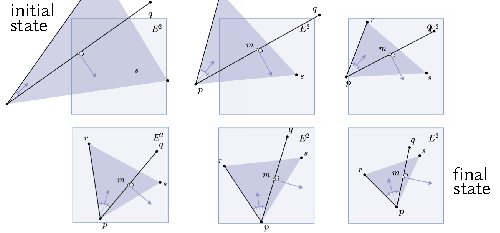
\includegraphics[scale=1.5]{assets/penrose/OptimizationProgress.pdf}
   \caption{Our solver can lay out diagrams even if we do not initially know how to satisfy all the constraints. Here we show several steps of optimization.\label{fig:OptimizationProgress}}
\end{figure}

\subsubsection{Initialization}

Just as a human diagrammer might consider several initial arrangements, we randomly sample several configurations and optimize only the most promising ones, \ie, the ones with the least overall energy in the exterior point problem.  Initial values are sampled uniformly at random from a range related to their types; for example, RGB color values are sampled from \([0,1]\).

\subsubsection{Failures and warnings}

Since our language framework is quite general, a programmer might define difficult or impossible optimization problems.  Hence, we can't guarantee that \Penrose{} produces a valid diagram.  However, the system can provide feedback by simply printing an error message if any of the constraint values are nonzero.  The resulting invalid diagram might even provide useful visual intuition for why the \Style\ program failed (\cref{fig:sets-inconsistent}).

\subsection{Plugins}
\label{sec:PlugIns}

A plugin is a piece of external code, written in any language, that is given information from a specific pair of \Substance\ and \Style\ files and can produce more \Substance\ and \Style\ information in specific files for \Penrose\ to use. A plugin is run when making diagrams with a particular \Style. A \Style\ may declare the plugins to be called at the top of the file with the syntax \mbox{\inlineSTY{\texttt{plugin "myPlugin" (args)}},} which states that the plugin \inlineSTY{\texttt{myPlugin}} should be run with the given argument list. When a diagram is generated, the plugin is given the \Substance{} program as a JSON file, as well as the parameters given in \Style\ as command-line arguments. The plugin can output new \Substance\ code as a text file and/or a set of values for the fields of any \Substance\ variable, encoded as a JSON file. The \Substance\ code generated by a plugin is appended to the existing \Substance\ program, and the values generated by the plugin can be accessed in \Style{} via the syntax \inlineSTY{\texttt{myPlugin[variable][field]}}. Note that a plugin is run exactly once, prior to execution of all \Penrose{} code. Therefore, the values generated by a plugin are not optimized by the layout engine, so plugin code does not have to be differentiable. For examples of plugin use, see \cref{sec:Functions} and \cref{sec:Meshes}.

% , including those \Substance\ variables generated by the plugin itself

\subsection{Rendering}
\label{sec:Rendering}

In this chapter we focused on generating 2D vector graphics, but in principle nothing about our system design limits us to this particular target.  For instance, the constraint-based approach is just as suitable for, say, generating arrangements of 3D objects that can be rendered via photorealistic ray tracing~\cite{Pharr:2016:PBR}, or even constrained interactive diagrams that could be used in virtual reality.  In our current implementation, graphical primitives are translated to SVG-native primitives via \emph{React.js}~\cite{Facebook:2020:RJS} and labels are postprocessed from raw \TeX\ to SVG paths using MathJax~\cite{Cervone:2012:MJ}.  Since \Penrose{} code is typically quite concise, we embed it as metadata into the SVG, easing reproducibility.  We also embed \Substance\ names as tooltips to improve accessibility.

\begin{figure}[t]
   \includegraphics[width=\columnwidth]{assets/penrose/PenroseIDE.jpg}
   \caption{Our system supports integration with web-based applications. Here a \Penrose\ IDE provides automatic syntax highlighting and autocomplete for any user-defined domain.\label{fig:PenroseIDE}}
\end{figure}

\subsection{Development Environment}
\label{sec:DevelopmentEnvironment}

To facilitate development, we built a web-based IDE (\cref{fig:PenroseIDE}) that highlights the potential for high-level diagramming tools built on \Penrose{}. For instance, since the \Domain{} grammar has a standard structure, the IDE can provide features like autocomplete and syntax highlighting for any domain. We are optimistic that the design choices made in \cref{sec:SystemDesign} will support the use of \Penrose{} as a platform for building diagramming tools beyond the use cases in this chapter.

 % and the ability to interactively manipulate elements of a generated diagram.
% Here, for instance, diagram elements can be dragged around the canvas and re-optimized to preserve the constraints (and hence meaning) of the given programs.  

\subsection{Implementation}
\label{sec:Implementation}

The \Penrose\ system is written in Haskell and the rendering frontend is written in Typescript. We wrote our own solver using the Haskell library \textit{ad}~\cite{autodiff:kmett} to perform automatic differentiation. We provide one output target and renderer (SVG), together with a fixed set of graphical primitives that are loosely based on SVG (\eg circles and paths), plus features that SVG users commonly add by hand, like arrowheads. We also provide a fixed set of objectives and constraints for specifying spatial layout, such as shape containment and adjacency relationships, and other functions for performing spatial queries, such as computing bounding boxes and pairwise distances. Sustained use by a community of users might point the way to a standard library. The system has been open-sourced here: \texttt{github.com/penrose/penrose}


\section{Examples and Evaluation}
\label{sec:ExamplesandEvaluation}

% GENERAL POINTS ABOUT EXAMPLES

% What are the *claims* that our examples support?
% First: there are several far-reaching claims on the first page… this approach has several broad-reaching benefits.
% Do our examples support those claims?
% Claim 1 (novices and notation). If we look at our examples, do they support this claim?
%     How do you convince someone this is familiar notation? Show snippets from some other textbook
%     Mention those four bullet points whenever we can
%     What you want to do is cut to the chase. Make the topic sentence about the system, and everything else a “for example.”
%     Make it clear that this is just an *example* and that it’s being used to illustrate a particular principle. Indicate that with phrases like "For example," "for instance," "to illustrate this principle," "just one example is"… They’re not really the example you’re talking about, just the supporting evidence. (?)

% Other example sections in systems papers:
% Section 5.2 https://arxiv.org/pdf/1910.02993.pdf
% Section 5.2 http://graphics.stanford.edu/papers/scanner/poms18_scanner.pdf

% \todo{Revise this introduction to discuss the broad claims}

Our main goal for \Penrose\ was to create a system that can automatically generate diagrams from many different domains using familiar syntax. Here we examine our design by exploring examples from a variety of common domains in mathematics and computer graphics; we also do some basic performance analysis (\cref{sec:PerformanceEvaluation}). 

% All examples in the paper were generated automatically and were not manipulated by hand. However, due to small errors when converting our SVG output to the PDF format required by \texttt{pdflatex}, minor manual editing was required (\eg{} fixing broken transparency).

% Though this process, we see that \Penrose{} programs allow us codify best practices of expert diagrammers in a way that be easily reused by non-expert users.
% ^ I'm not sure if we can support this claim...

% TODO Say something like: Being able to make lots of diagrams easily makes it that much easier to make "microdiagrams" that clearly illustrate one small idea, rather than feeling like diagrams have to be saved for only the most critical concepts, or packed full of lots of different ideas.

% TODO Discuss package used to draw our computational graphs; draw a comparison to GraphViz, pointing out that our general solution easily provides much of the core functionality of their entire specialized solution (at least from a language point of view).

\subsection{Sets}
\label{sec:Sets}

% \setlength{\columnsep}{1em}
% \setlength{\intextsep}{0em}
% \begin{wrapfigure}{l}{140pt}
\begin{figure}
   \centering
   \includegraphics[width=.7\linewidth]{assets/penrose/life.pdf}
   \caption{Two \Style{} programs illustrate classification of life in biology as an Euler diagram (\figloc{left}) and a tree diagram (\figloc{right}).}
   \label{fig:set-life}
\end{figure}
% \end{wrapfigure}\vspace{-\baselineskip}

A simple example that illustrates many principles of our system design is the domain of basic set theory---\cref{fig:set-styles} shows a complete listing for one of three possible styles.  Notice here the complete absence of explicit coordinates in both the \Substance{} and \Style{} code.  The other two \Style{} programs (not shown) either improve the visual styling, or shift to a different representation where subset inclusion is indicated by a tree-like drawing rather that overlapping disks.  Different representations are especially helpful for different types of examples---for instance, disks must shrink exponentially for deeply nested subsets (\cref{fig:set-life}, \figloc{left}), whereas a tree diagram remains easy to read (\cref{fig:set-life}, \figloc{right}). One limitation highlighted by this example is that the constraints and objectives appearing in \Style{} are not yet extensible within the language itself---for instance, the statement \inlineSTY{\keyword{ensure} \texttt{contains(y.shape,x.shape)}} translates to a fixed function on the centers and radii of the two disks.

This example also demonstrates the benefit of a more explicit type system, rather than, say, interpreting raw mathematical strings as in \TeX.  In particular, \cref{fig:enumerate-subsets} shows how a \Domain{} schema can be used with program synthesis techniques (\cref{sec:LargeScaleDiagramGeneration}) to automatically enumerate different \emph{logical} instantiations of the given \Substance{} code.  To make this example, there was no need to model sets as an explicit datatype (\eg\ a list of points) nor to assign semantics to these datatypes (such as the impossibility of two sets being both intersecting and nonintersecting). Instead, the program synthesizer can reason purely about the abstract types specified in the \Domain\ schema, letting the constraints defined in the \Style{} define the visual semantics. Thus, the program synthesizer can check if the generated code is valid by simply testing if the constraints defined in \Style{} all evaluate to zero for the optimized diagram.  This example captures an important aspect of our system design: the mapping defined by \Style{} programs not only provides a superficial visual interpretation, but also assigns deeper mathematical meaning.

\begin{figure}[ph]
\begin{minipage}[t]{\columnwidth}
\begin{mdframed}[style=DSLCode]
\begin{lstlisting}[language=Elem,escapechar=@,numbers=none]
type Set                                                             -- Sets.dsl
predicate Intersecting : Set s1 * Set s2
predicate IsSubset : Set s1 * Set s2
predicate Not : Prop p
notation "A $\subset$ B" ~ "IsSubset(A, B)"
notation "A $\cap$ B = $\varnothing$" ~ "Not(Intersecting(A, B))"
\end{lstlisting}
\end{mdframed}
\end{minipage}
\begin{mdframed}[style=SUBCode]
\begin{minipage}[t]{0.5\columnwidth}
\begin{lstlisting}[language=Sub-SET,escapechar=@,numbers=none]
Set A, B, C, D, E, F, G
B $\subset$ A
C $\subset$ A
D $\subset$ B
E $\subset$ B
\end{lstlisting}
\end{minipage}
\ContinueLineNumber
\begin{minipage}[t]{.5\columnwidth}
\begin{lstlisting}[language=Sub-mesh,escapechar=@,numbers=none]
F $\subset$ C                      -- Sets.sub
G $\subset$ C
E $\cap$ D = $\varnothing$
F $\cap$ G = $\varnothing$
B $\cap$ C = $\varnothing$
\end{lstlisting}\end{minipage}\end{mdframed}
\vspace{-.9\baselineskip}
\begin{minipage}[t]{\columnwidth}
\begin{mdframed}[style=STYCode]
\begin{lstlisting}[language=Sty-ST,escapechar=@,numbers=none]
forall Set x {                                                 -- Sets-Disks.sty 
    x.shape = Circle { strokeWidth : 0.0 }
    x.text = Text { string : x.label }
    ensure contains(x.shape, x.text)
    encourage sameCenter(x.text, x.shape)
    layer x.shape below x.text
}
forall Set x; Set y
where IsSubset(x, y) {
    ensure contains(y.shape, x.shape)
    ensure smallerThan(x.shape, y.shape)
    ensure outsideOf(y.text, x.shape)
    layer x.shape above y.shape
    layer y.text below x.shape
}
forall Set x; Set y
where NotIntersecting(x, y) {
    ensure disjoint(x.shape, y.shape)
}\end{lstlisting}\end{mdframed}\end{minipage}
\begin{minipage}[t]{\columnwidth}
\includegraphics[width=\columnwidth]{assets/penrose/set-styles.pdf}
\end{minipage}
   \caption{Here, some \Substance{} code is used to specify set relationships. Different \Style{} programs not only tweak the visual style (\eg flat vs. shaded disks), but allow one to use a completely different visual representation (\eg a tree showing set inclusions).  \texttt{Sets.sty} above describes the flat disk style.\label{fig:set-styles}}
\end{figure}


\subsection{Functions}
\label{sec:Functions}

\begin{figure}
   \centering
   \begin{minipage}[t]{0.33\columnwidth}
      \begin{mdframed}[style=SUBCode]
      \begin{lstlisting}[language=Sub-ST,escapechar=@,numbers=none]
-- Injection.sub
Set A, B
f: A -> B
Injection(f)
Not(Surjection(f))\end{lstlisting}
      \end{mdframed}
   \end{minipage}\hfill\begin{minipage}[t]{0.32\columnwidth}
      \begin{mdframed}[style=SUBCode]
      \begin{lstlisting}[language=Sub-ST,escapechar=@,numbers=none]
-- Surjection.sub
Set A, B
f: A -> B
Surjection(f)
Not(Injection(f))\end{lstlisting}
      \end{mdframed}
   \end{minipage}\hfill\begin{minipage}[t]{0.30\columnwidth}
      \begin{mdframed}[style=SUBCode]
      \begin{lstlisting}[language=Sub-ST,escapechar=@,numbers=none]
-- Bijection.sub
Set A, B
f: A -> B
Surjection(f)
Injection(f)\end{lstlisting}
      \end{mdframed}
   \end{minipage}
   \begin{minipage}[t]{\columnwidth}    
   \centering
   \includegraphics[scale=1.5]{assets/penrose/func-continuous-discrete-vert.pdf}
   \end{minipage}
   \caption{Different visual representations provide different ways of thinking about an idea.  Here, the notion of injections, bijections, and surjections is illustrated in both discrete \figloc{(left)} and continuous \figloc{(right)} styles.  In the former, functions with the desired properties are randomly generated by an SMT solver, allowing the user to learn from many different examples.\label{fig:substance-fn-images}}
\end{figure}


% predicate Injection : Map m
% predicate Surjection : Map m
% predicate Bijection : Map m
% predicate PairIn : Point * Point * Map

   A natural concept to build on top of sets is mappings between sets. This example also illustrates the use of plugins (\cref{sec:PlugIns}).  We first add a \inlineDSL{\keyword{Map}} type to the \Domain{} for sets (\cref{sec:Sets}), as well as a constructor \inlineDSL{\texttt{From: Set * Set -> Map}} specifying the domain and codomain of the map.  Here, syntactic sugar\vspace{.5\baselineskip}

   \noindent\inlineDSL{\keyword{notation} \texttt{"f: A -> B" ~ "Map f; From(f, A, B)"}}\vspace{.5\baselineskip}

   \noindent enables one to both declare and define the map via the concise, familiar notation \inlineSUB{\texttt{f: A -> B}}.  In \cref{fig:substance-fn-images} we add predicates \inlineDSL{\keyword{Injection}}, \inlineDSL{\keyword{Surjection}}, and \inlineDSL{\keyword{Bijection}} to the \Domain{} schema to illustrate some basic ideas about maps.  The two different styles of illustration help ease the transition from thinking of mappings between discrete points to thinking of continuous mappings on the real line.  To generate the discrete examples, we wrote a plugin (\cref{sec:PlugIns}) that acts as ``glue'' between \Penrose{} and an external SMT solver (another example is shown in \cref{fig:FunctionComposition}).  The compiler uses this plugin to expand the \inlineSUB{\keyword{Map}} objects from \cref{fig:substance-fn-images}, \figloc{top} into specific instances of a new \inlineSUB{\keyword{Point}} type, as well as a new predicate \inlineSUB{\texttt{(a, b) \(\in\) f}} that expresses a map as an explicit list of domain/codomain pairs.  For instance, the map in \cref{fig:substance-fn-images} generates points \inlineSUB{\texttt{\keyword{Point} A0, A1, B0, B1, B2}} with the two predicates \inlineSUB{\texttt{(A0, B1) \(\in\) f}} and \inlineSUB{\texttt{(A1, B2) \(\in\) f}}.  A \Style{} tailored to these types is used to generate diagrams in \cref{fig:substance-fn-images}, \figloc{left}; as in \cref{fig:sets-color-opt}, hue is optimized to enhance contrast between nearby points.  In contrast, the continuous function diagrams in \cref{fig:substance-fn-images}, \figloc{right} do not require an external plugin, but instead constrain the degrees of freedom of a B\'{e}zier curve.  Finally, \cref{fig:FunctionComposition} shows how abstract function composition in \Substance{} is automatically translated into explicit composition of generated functions by the \Style\ program without any \Substance{} writer effort.

% \todo{Revise programs in the functions-domain folder to reflect the Substance programs in the figure}

\begin{figure}
   \centering
   \begin{minipage}{160pt}
      \begin{mdframed}[style=SUBCode]
         \begin{lstlisting}[language=Sub-ST,escapechar=@,numbers=none]
Set A, B, C
f: A -> B
g: B -> C
Injection(f)
Bijection(g)
Function gf = g(f)\end{lstlisting}
      \end{mdframed}
   \end{minipage}\hfill
   \begin{minipage}[c]{240pt}
      \includegraphics[width=.8\linewidth]{assets/penrose/FunctionComposition.pdf}
   \end{minipage}
   \caption{Here, abstract function composition is realized as explicit composition of functions produced via an SMT solver, illustrating the fact that the composition of an injection and a bijection is an injection. \label{fig:FunctionComposition}}\vspace{-\baselineskip}
\end{figure}

\subsection{Geometry}
\label{sec:Geometry}


Classical geometric figures provide a good opportunity to examine how one can use different \Style{} programs to change not only the superficial style of a diagram, but also its fundamental visual representation.  The familiar ``two-column proof'' exemplifies how, in mathematics, one can make geometric statements without referring to explicit quantities like coordinates and lengths.  Likewise, compass-and-ruler constructions (dating back to the ancient Greeks) show how geometric figures can be specified with only relative constraints.  These modalities are well-captured in the way we write \Substance{} and \Style{} code for geometric diagrams, respectively.  For instance, \cref{fig:ThreeEuclideanStyles}, \figloc{top} gives a listing of geometric assertions that resemble the left column in a two-column proof. This would likely be a natural notation even for intermediate-level students.  A bare-bones \Style{} program for this domain (not shown) comprises basic statements very similar to those used in \cref{fig:style_linalg}, \eg to express the orthogonality of two segments.  (This approach is similar to the special-purpose geometry package \emph{GCLC}~\cite{Janivcic:2006:GCLC}; however, here the domain of objects and visual representations are both extensible at the language level.)

\setlength{\columnsep}{1em}
\setlength{\intextsep}{0em}
\begin{wrapfigure}{l}{150pt}
   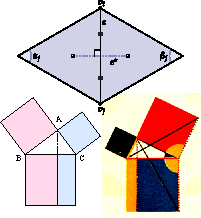
\includegraphics[width=\linewidth]{assets/penrose/EuclideanStyleInspiration.pdf}
   \caption{Diagrams used as inspiration for the \Style{}s in \cref{fig:ThreeEuclideanStyles}.}
 \end{wrapfigure}
\setlength{\intextsep}{1em}


One goal of \Penrose{} is to codify the subjective style choices made by professional illustrators so non-expert users can benefit from their expertise.  \cref{fig:ThreeEuclideanStyles}, \figloc{bottom} cascades on the bare-bones \Style{} program to riff on styles from several existing sources (shown in inset), namely, \emph{Byrne's Euclid}~\cite{Byrne:1847:FSB}, \emph{Wikipedia}~\cite{Wikimedia:2006:IEP}, and a collection of illustrated notes on \emph{discrete differential geometry}~\cite{Crane:2013:DGP}. This figure also illustrates how we can ``mix and match'' different \Style{} and \Substance{} programs. The bulk of these styles (\(\sim\)500 lines) share the same baseline Style code; additional code for a specific style requires less than 100 more lines. To illustrate the Pythagorean theorem (right column), we also used cascading to add diagram-specific features (\eg altitude and extension lines).

\begin{figure}
  \centering

  \begin{minipage}[c]{0.41\columnwidth}  
  \begin{mdframed}[style=SUBCode]
  \begin{lstlisting}[language=Sub-geom,escapechar=@,numbers=none]
Point A, B, C
-- define a right triangle
Triangle ABC := {A,B,C}
Angle $\uptheta$ := $\angle$(C,A,B)
Right($\uptheta$)
-- square each side
Point D, E, F, G, H, I
Square CBDE := [C,B,D,E]
Disjoint(CBDE, ABC)
Square BAGF := [B,A,G,F]
Disjoint(BAGF, ABC)
Square ACIH := [A,C,I,H]
Disjoint(ACIH, ABC
-- split hypotenuse area
Segment AK := Altitude(ABC,$\uptheta$)
Point K := Endpoint(AK)
Segment DE := {D,E}
Point L
On(L, DE)
Segment KL := {K,L}
Perpendicular(KL, DE)
Rectangle BDLK := {B,D,L,K}
Rectangle CKLE := {C,K,L,E}
-- (plus additional objects
-- from Byrne's diagram)\end{lstlisting}
\end{mdframed}
\end{minipage}\hfill
\begin{minipage}[c]{.58\columnwidth}
  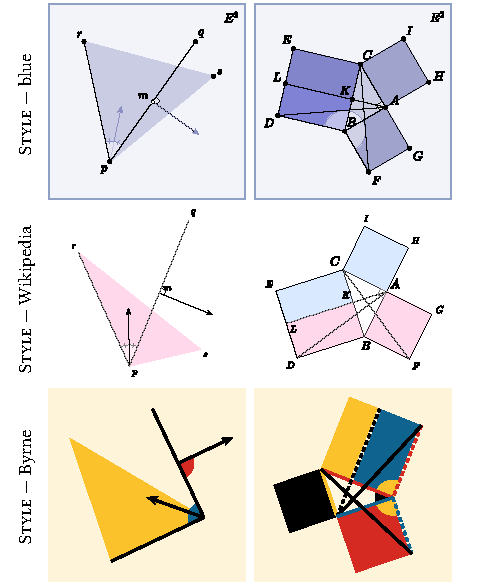
\includegraphics[width=\linewidth]{assets/penrose/ThreeEuclideanStyles.pdf}
\end{minipage}
   \caption{The cascading design of \Style{} enables one to modify a base style with relatively little code.  Here the two \Substance{} programs from \cref{fig:teaser} and the listing above are visualized in three different styles, all of which build on the same basic constraints and objectives.\label{fig:ThreeEuclideanStyles}}\vspace{-\baselineskip}
\end{figure}

In the spirit of Hilbert's quip (\cref{sec:SystemDesign}), we can also swap out the basic visual representation of a given set of logical statements.  For instance, any collection of geometric statements that does not assume the \emph{parallel postulate}  can be realized in several different geometries (\cref{fig:teaser}).  To generate this figure, we wrote three \Style{} programs that all match on the same patterns from a common ``neutral geometry'' \Domain{} schema.  Swapping out these \Style{} files then allows users to build intuition about spherical or hyperbolic geometry by exploring how a given figure (expressed via \Substance{}) differs from its Euclidean counterpart.  Such an example could be further enriched by writing styles for different models of hyperbolic geometry (such as half-plane, hyperboloid, or Beltrami-Klein), each of which involves meticulous calculations.  

% To show that these examples were not cherry-picked, \cref{fig:GeometrySamples} depicts a gallery of samples.

Finally, the diagram specification enables us to build ``staged'' diagrams, such as ones illustrating the steps of a proof.  \cref{fig:byrne-stages} successively uncomments lines of \Substance{} code to produce a style of explanation common in textbooks and slides, a strategy which could easily be applied to (say) any two-column proof. In this example, the values of optimized variables are fixed by hand; an interesting question is how this might be done automatically.

% TODO include a Style listing for the three Style programs in the supplemental material?
% TODO: Compare the code and resulting images to a diagram made in other geometry libraries?


\begin{figure}[t]
   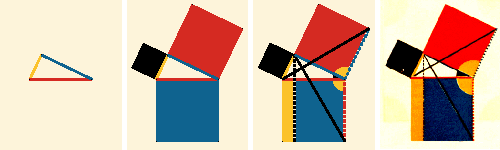
\includegraphics[width=\columnwidth]{assets/penrose/byrne-stages.pdf}
   \caption{Once a complex diagram has been built, it can be easily broken into pieces or stages by, \eg commenting out lines of \Substance{} code.  Here we illustrate steps in Euclid's proof of the Pythagorean theorem, turning Byrne's static figure \figloc{(far right)} into a progressive ``comic strip.''\label{fig:byrne-stages}}
 \end{figure}
 

\subsection{Linear Algebra}
\label{sec:LinearAlgebra}

% (Should we say that doing this creates new capabilities?)
% The difference in \Substance{} is that strings are written by a programmer to convey a mathematical meaning, not automatically generated by production rules.

In mathematics, complexity is built up by composing simple statements. The mapping defined by a \Style{} program automatically lifts this \emph{compositionality} to the visual setting. That is, it enables \Substance\ writers to compose logical statements to build up visual complexity without explicit effort from the \Style{} programmer.  A good analogy is procedural \emph{L-systems}~\cite{Prusinkiewicz:2012:ABP}. Although a graphics programmer can directly write code to recursively apply spatial transformations, it saves effort to first generate strings in a grammar, then systematically translate these strings into graphical transformations.

In \Penrose{}, examples from linear algebra demonstrate compositionality.  The \Style{} declaration on Line~\ref{lin:VectorIsALittleArrowEnd} of \cref{fig:style_linalg} defines the visual icon for a vector (a 2D arrow).  Suppose we now want to illustrate \emph{linear maps}, denoted by \(f\), which have two defining properties: linearity of vector addition (\(f(u+v) = f(u)+f(v)\) for all vectors \(u,v\)) and homogeneity of scalar multiplication (\(f(cu) = cf(u)\) for all vectors \(u\) and scalars \(c\)).  Successive \Style\ rules cascade on \cref{fig:style_linalg} to define how these logical operations  should be mapped to visual transformations.  For example, application of a linear map \(f\) is represented by a literal $2 \times 2$ matrix-vector multiply; the image vector \(f(u)\) also inherits the color of the argument \(u\). The map itself is visually represented by a labeled arrow, and the domain and target spaces by coordinate planes on either side. The \Style{} programmer need not compose these directives explicitly; the compiler does the tedious job of translating \Substance{} statements (\cref{fig:linearMap}, \figloc{top}) into a composition of graphical statements that define a diagram (\cref{fig:linearMap}, \figloc{bottom}).  Moreover, since the \Style{} program faithfully represents the underlying mathematics, we observe the expected properties, \eg the arrow for \(f(u_1+u_2)\) is the same as the arrow for \(f(u_1)+f(u_2)\).  Automatically checking consistency of the visual representation based on analysis of a richer \Domain{} schema would be an interesting topic for future work.

% (addition, scaling, and application of linear maps)
% \setlength{\columnsep}{1em}
% \setlength{\intextsep}{0em}
% \begin{figure}{l}{140pt}
\begin{center}
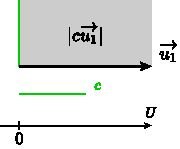
\includegraphics[width=140pt]{assets/penrose/LinearAlgebra1D.pdf}
\end{center}
% \end{wrapfigure}

Finally, the inset (above) shows an alternative representation for vectors and scalars as signed and unsigned quantities ($u_1$ and $c$, \resp{}) on the number line.  The benefit of a 1D representation is that the remaining dimension can be used to illustrate different concepts, in this case relating the magnitude of a product to an area.  The ability to switch between representations can be pedagogically valuable, such as for transitioning from lower to higher mathematics.

\begin{figure}
  \begin{minipage}[t]{0.45\columnwidth}
   \begin{mdframed}[style=SUBCode]
    \begin{lstlisting}[language=Sub-LA,escapechar=@,numbers=none]
VectorSpace U, V
LinearMap f : U $\rightarrow$ V
Vector u1, u2, u3 $\in$ U
Vector v1, v2, v3, v4 $\in$ V
u3 := u1 + u2
v1 := f(u1)
v2 := f(u2)
v3 := f(u3)
v4 := v1 + v2
\end{lstlisting}
   \end{mdframed}
\end{minipage}\hfill
  \begin{minipage}[t]{0.45\columnwidth}
   \begin{mdframed}[style=SUBCode]
    \begin{lstlisting}[language=Sub-LA,escapechar=@,numbers=none]
VectorSpace U, V
LinearMap f : U $\rightarrow$ V
Vector u1, u2 $\in$ U
Vector v1, v2, v3 $\in$ V
Scalar c
u2 := c * u1
v1 := f(u1)
v2 := f(u2)
v3 := c * v1 \end{lstlisting}
   \end{mdframed}
  \end{minipage}
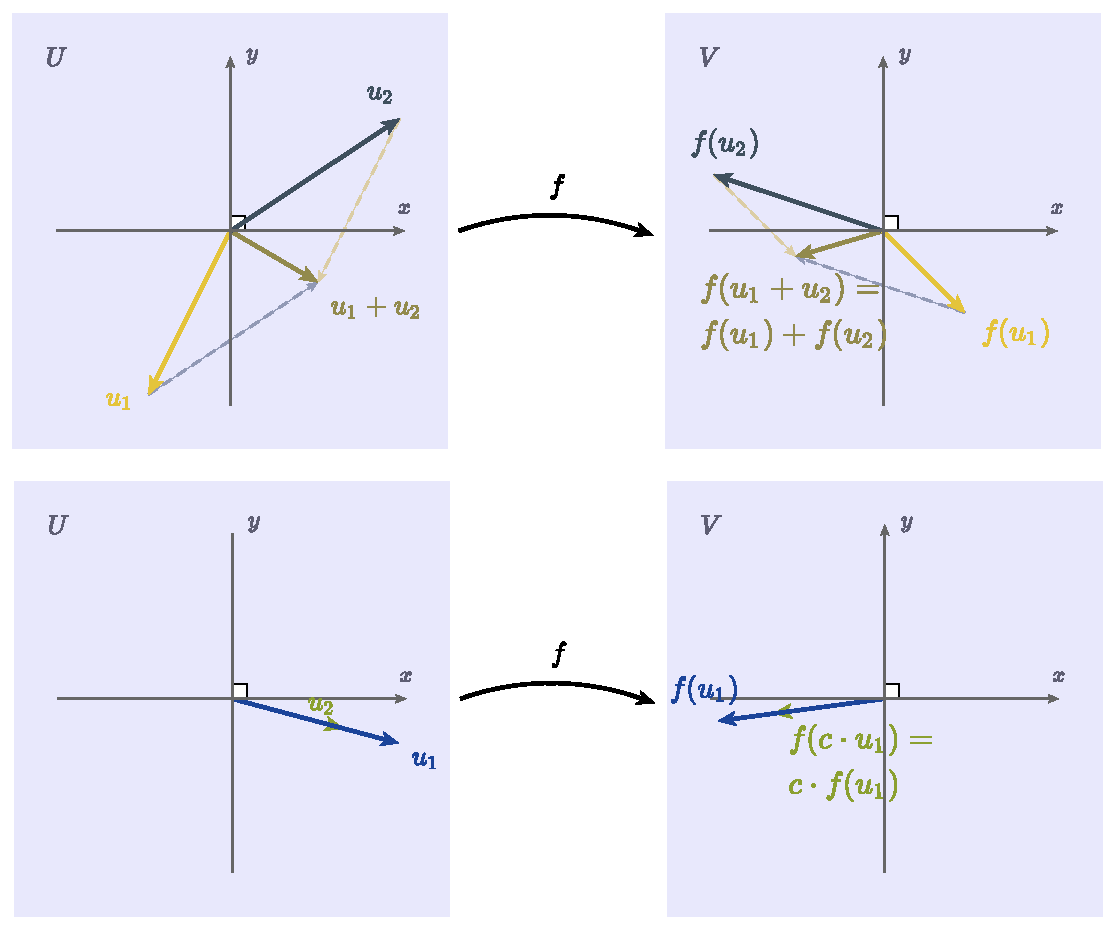
\includegraphics[width=\columnwidth]{assets/penrose/linearmap-add-scale.pdf}
   \caption{Composition of mathematical statements naturally translates into composition of graphical transformations with no explicit programmer effort.  Here we compose linear maps, showing addition and scaling, to illustrate the two defining properties of linear maps.\label{fig:linearMap}}
\end{figure}


% AutoLabel All
% Label u1 $u_1$
% Label u2 $u_2$
% Label u3 $u_1 + u_2$
% Label v1 $f(u_1)$
% Label v2 $f(u_2)$
% Label v3 $f(u_1 + u_2) = \\ f(u_1) + f(u_2)$
  
% \todo{Fix the label strings above so they aren't typeset?}

% AutoLabel All
% Label u1 $u_1$
% Label u2 $u_2$
% Label v1 $f(u_1)$
% Label v2 $f(c \cdot u_1) = \\ c \cdot f(u_1)$
% Label v3 $f(c \cdot u_1) = \\ c \cdot f(u_1)$      

%   \begin{overpic}[scale=0.4]{assets/penrose/linalg-vectorsadd3.pdf}
%     \put(2,80) {\parbox{2in}{
%         \texttt{\textbf{VectorSpace} U} \\
%         \texttt{\textbf{Vector} u1, u2, u3,} \\
%         \texttt{\mbox{              } u4, u5} \\
%         \texttt{u3 := u1 + u2} \\
%         \texttt{u5 := u3 + u4}
%         }}
%     \end{overpic}
% \caption{A simple \Substance{} program that specifies that several vectors are added results in a gallery of diagrams illustrating the given relationships. \label{fig:PenroseWorkingLA}}

\begin{figure}
\begin{mdframed}[style=SUBCode]
\begin{minipage}[t]{.47\columnwidth}
\begin{lstlisting}[language=Sub-mesh,escapechar=@,numbers=none]
SimplicialComplex K
Edge e $\in$ K
Subcomplex E $\subseteq$ K
E := Closure(e)
SimplicialSet StE $\subseteq$ K
StE := Star(E)
Subcomplex ClStE $\subseteq$ K
\end{lstlisting}
\end{minipage}
\ContinueLineNumber
\begin{minipage}[t]{.5\columnwidth}
\begin{lstlisting}[language=Sub-mesh,escapechar=@,numbers=none]
ClStE := Closure(StE)
Subcomplex ClE $\subseteq$ K
ClE := Closure(E)
SimplicialSet StClE $\subseteq$ K
StClE := Star(ClE)
SimplicialSet LkE $\subseteq$ K
LkE := SetMinus(ClStE, StClE)\end{lstlisting}
\end{minipage}
\end{mdframed}
   \centering
   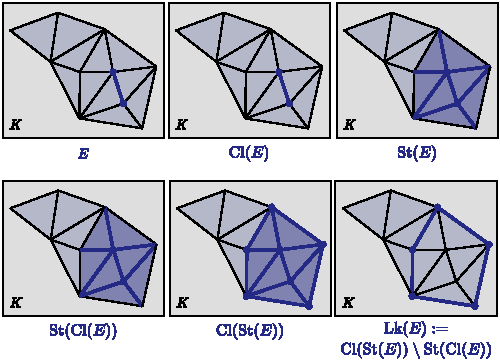
\includegraphics[scale=1.5]{assets/penrose/mesh-figure.pdf}
   \caption{A language-based specification makes it easy to visually inspect data structures or assemble progressive diagrams with only minor changes to program code.  Here we draw the simplicial \emph{link} by building it up from simpler constituent operations.\label{fig:substance-mesh-clst}}
\end{figure}

\begin{figure}
   \centering
   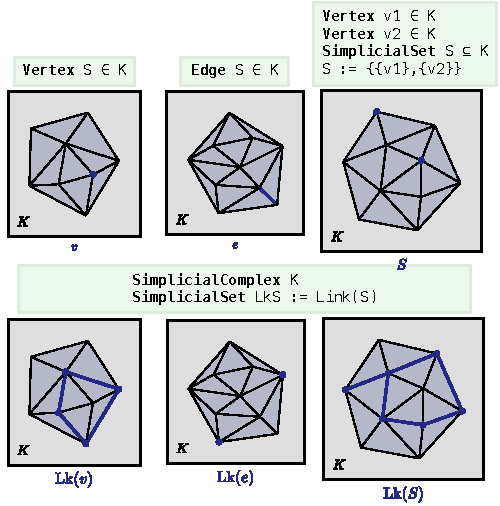
\includegraphics[scale=1.5]{assets/penrose/mesh-examples.pdf}
   \caption{Domain-specific notation makes it easy to explore an idea by trying out many different examples.  Here several subsets of a simplicial complex are specified \figloc{(top)} to explore the definition of the ``link'' \figloc{(bottom}).  An external plugin generates random example meshes, further enriching exploration.\label{fig:mesh-examples}}
\end{figure}

\subsection{Meshes}
\label{sec:Meshes}

Polygonal meshes are ubiquitous in computer graphics, but illustrating meshes is often cumbersome due to the large number of elements involved, especially when illustrating meshes by hand or in GUI-based tools.  In such cases, \Penrose{} can be useful not just for making illustrations, but also to inspect and debug user-defined data structures by attaching them to custom visualizations.  A simple example is shown in \cref{fig:substance-mesh-clst}, where different regions of a mesh are specified via standard operators on a simplicial complex; this diagram also illustrates the definition of the simplicial \emph{link}~\cite[Section 3.3]{Bloch:1997:FCG}.  Further examples in \cref{fig:mesh-examples} show how a user can quickly build intuition about this definition by drawing the link of a variety of different mesh subsets.

To make these examples in \Penrose{}, we follow a pattern similar to the discrete function example (\cref{sec:Functions}): generic mesh objects from the \Substance{} code are refined into specific instances of \inlineSUB{\keyword{Vertex}}, \inlineSUB{\keyword{Edge}}, and \inlineSUB{\keyword{Face}} objects by an external plugin, which generates and optimizes a random triangle mesh.  Since meshes are randomly generated, the plugin passes a random seed (from its \Style{} arguments) to draw different pieces of the same mesh.  For this example, we used an existing JavaScript-based mesh processing library~\cite{Sawhney:2017:GPJ} that was not designed ahead of time to interface with \Penrose{}.  The benefit of generating these elements at the \Substance{} level (rather than returning, say, a static SVG image) is that they can continue to be styled and manipulated within \Penrose{}; the programmer does not have to edit extra graphics code or keep it compatible with the \Style{} program.  Likewise, programmers who adopt \Penrose{} as a tool for visual debugging can benefit from system improvements while writing minimal code to attach their data structures to a visual representation.

% AutoLabel E
% AutoLabel e
% AutoLabel K
% Label S1 $\mathrm{St}(E)$
% Label A $\mathrm{Cl}(\mathrm{St}(E))$
% Label B $\mathrm{Cl}(E)$
% Label S2 $\mathrm{St}(\mathrm{Cl}(E))$
% Label S3 $\mathrm{Lk}(E) := \mathrm{Cl}(\mathrm{St}(E)) \setminus \mathrm{St}(\mathrm{Cl}(E))$
% Label S4 $\mathrm{Lk}(E)$
% SimplicialSet S4 $\subseteq$ K
% S4 := Link(E)

% Result(E) -- Cl(e)
% Result(B) -- Cl(E)
% Result(S1) -- Star(E)
% Result(A) -- Cl(S1)
% Result(S2) -- St(B)
% Result(S4) -- Lk(E)

%%%%%%%%%%

% SimplicialComplex K
% Vertex v1 $\in$ K
% Vertex v2 $\in$ K
% SimplicialSet S $\subseteq$ K
% S := Union(v1, v2)
% SimplicialSet S1 $\subseteq$ K
% S1 := Link(S)
% Result(S1)
     
\subsection{Ray Tracing}
\label{sec:RayTracing}

\begin{figure}
   % PathType t1, t2, t3
   % HasForm (t1, "L(D|S)SE")
   % HasForm (t2, "LSDE")
   % HasForm (t3, "LE")

   % Path p1, p2, p3
   % p1 := Sample(t1)
   % p2 := Sample(t2)
   % p3 := Sample(t3)
   \centering
   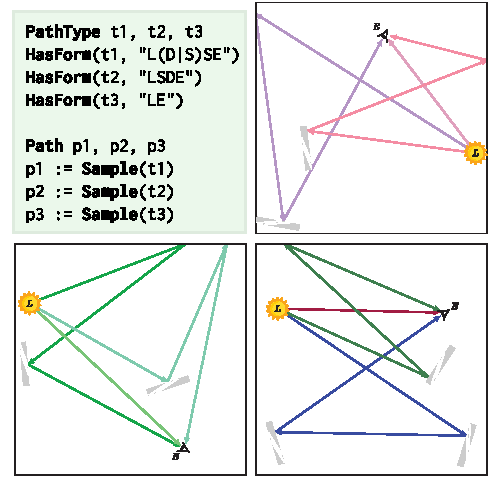
\includegraphics[scale=1.5]{assets/penrose/rt-multiple-paths.pdf}
   \caption{When drawing ray tracing diagrams by hand, it can be difficult to construct geometry that permits the desired path types.  Here we jointly optimize path and scene geometry to match multiple path types simultaneously.  Shown are several diagrams generated for the same program. A specular reflection (\texttt{S}) is represented as a mirror reflection, whereas a diffuse reflection (\texttt{D}) is represented as a bounce off of one of the walls. \label{fig:rt-multiple-paths}}
\end{figure}


Our final example constructs light path diagrams, which are often used to illustrate ideas in physically-based rendering.  The \Substance{} code expresses types of light paths via Heckbert's regular expression notation.  For instance, the expression \inlineSUB{\texttt{L(D|S)S*E}} specifies a family of light paths that start at a light source (\inlineSUB{\texttt{L}}), bounce off a diffuse or specular object (\inlineSUB{\texttt{S|D}}), then bounce off zero or more specular objects (\inlineSUB{\texttt{S*}}), then enter the ``eye'' or camera (\inlineSUB{\texttt{E}}).  One or more paths can then be declared that have a given form (\cref{fig:rt-multiple-paths}).  The challenge in generating a diagram from such a specification is that there must be geometry in the scene that supports the given path(s).  For instance, for a fixed eye, light, and mirror, there may simply be no path of the form \texttt{LSE}.  Rather than meticulously constructing a valid scene by hand, we can use a \Style{} program to jointly optimize the scene geometry and the light path by specifying constraints such as equality of incoming and outgoing angles at a specular bounce.  The set of objects in the scene is generated by a simple plugin that expands the regular expression into a set of compatible objects (\eg a mirror for each specular bounce).  This plugin also uses the canvas size to choose appropriate scene and path complexity according to the target output device (\cref{fig:Retargeting}).  Diagrams for more intricate light transport phenomena could be generated by calling an actual ray tracer (such as \emph{PBRT}~\cite{Pharr:2016:PBR}) to trace and rejection-sample paths by path type.  The added value of generating the final diagrams with \Penrose{} is that initial path and scene geometry generated by the external code can be further optimized to meet other design goals, such as the canvas size. Additionally, the visual style of a large collection of diagrams (\eg for a set of course notes) can easily be adjusted after the fact.

In our experience, \Penrose{} acts as a \emph{nexus} for diagram generation. It connects disparate components, such as language-based specification and ray tracing, into a diagramming tool that provides the system-level benefits described in \cref{sec:Introduction}.



% This is the selector for positioning the mirror for a specular bounce, which is interesting but too long/involved to include

% PathEdge e1; PathEdge e2; Path ps
% where e1 := CreateEdge(v1, v2);
%       e2 := CreateEdge(v2, v3);
%       IsSpecular(v2); Hits(v2, o)
% with PathVertex v1, v2, v3; SpecularObject o {
%     LOCAL.mirrorPadding = 1.0
%     LOCAL.horizontalShift = sampleReal(o.shape.w / -2.0 + 20.0, o.shape.w / 2.0 - 20.0)
%     override o.shape.rotation = mirrorAngle(e1.shape, e2.shape)
%     override o.shape.x = mirrorPosX(e1.shape, e2.shape, v2.x, v2.y, o.shape.h / 2.0 + LOCAL.mirrorPadding, LOCAL.horizontalShift)
%     override o.shape.centerY = mirrorPosY(e1.shape, e2.shape, v2.x, v2.y, o.shape.h / 2.0 + LOCAL.mirrorPadding, LOCAL.horizontalShift)
%   }

% \begin{figure}
%   \begin{overpic}[scale=0.15]{assets/penrose/rt-samples.pdf}
%       \put(-5,75) {\parbox{2in}{
%           \texttt{\textbf{PathType} t} \\
%           \texttt{\textbf{HasForm}(t,"L(D|S)S*E")} \\
%           \texttt{\textbf{Path} p := \textbf{Sample}(t)}
%         }}
%     \end{overpic}
%         \caption{ \label{fig:rt-samples}}
% \end{figure}

% \begin{figure}
%   \begin{minipage}[!t]{.4\columnwidth}
%   \begin{lstlisting}[language=Sub-RT,escapechar=@]
% PathType t1, t2, t3
% HasForm(t1, "L(D|S)SE")
% HasForm(t2, "LSDE")
% HasForm(t3, "LE")

% Path p1, p2, p3
% p1 := Sample(t1)
% p2 := Sample(t2)
% p3 := Sample(t3) \end{lstlisting}
% \end{minipage}\begin{minipage}[!t]{.6\columnwidth} 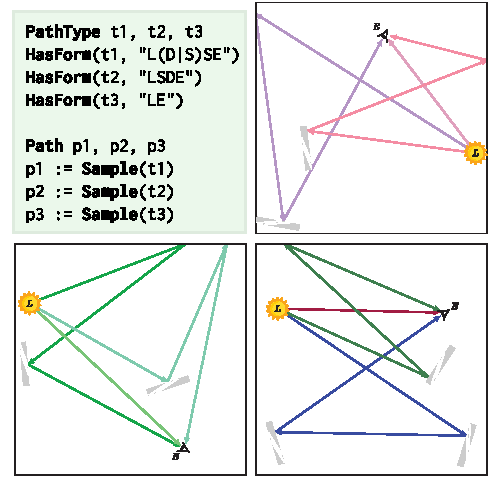
\includegraphics[width=\columnwidth]{assets/penrose/rt-multiple-paths.pdf}
% \end{minipage}
% \caption{When drawing ray tracing diagrams by hand, it can be difficult to construct scene geometry that permits the desired types of paths. With our optimization based layout, objects in the scene can be automatically arranged to satisfy complex path descriptions. Here we show a scene that simultaneously supports several different path types. \label{fig:rt-multiple-paths}}
% \end{figure}

\subsection{Large-Scale Diagram Generation}
\label{sec:LargeScaleDiagramGeneration}

One goal for \Penrose{} is that effort spent on diagramming should be generalizable and reusable (\ref{gol:Reuse}). To demonstrate the system's reuse potential, we developed a simple program synthesizer to automatically create any number of diagrams randomly sampled from a domain. The synthesizer is a simpler version of the \Edgeworth mutation algorithm (\cref{alg:mutation}): given a \Domain{} program, a \Style{} program, and the number of diagrams (\textsf{n}) as input, the synthesizer analyzes the \Domain{} program to find the mathematical constructs in the domain, randomly creates \textsf{n} \Substance{} programs that contain these constructs, then compiles, optimizes, and renders the results. \cref{fig:enumerate-subsets} demonstrates an example of using the synthesizer to ``autocomplete'' an underspecified \Substance{} program by automatically enumerating all possible subset relationships, using information from the \Domain\ schema. Automatically generating diagrams at scale can also help users write better \Style{} programs, since synthesizer can ``fuzz'' the space of possible \Substance{} programs to find corner cases.

To stress-test the system's performance and the reusability of \Style{} and \Domain{}\ programs, we randomly generated 2000 \Substance{} programs from the sets domain (\cref{sec:Sets}) in the flat disc style. \Penrose{} was able to create diagrams for all samples. Though 1058 of the 2000 programs had conflicting constraints due to randomness, the solver failed gracefully (as in \cref{fig:sets-inconsistent}) and reached convergence.

\subsection{Performance Evaluation}
\label{sec:PerformanceEvaluation}

We hope to support an iterative workflow where the system's performance does not block the user's creative process. One possible goal is to generate most diagrams within ten seconds, since that threshold is deemed a ``unit task'' in cognitive science~\cite{unifiedTheoriesCognition} and is about as long as similar authoring processes take, such as building a \LaTeX{} document or compiling code. Even lower latency ($<$ 500 ms) might enable new applications of \Penrose, since this threshold benefits users of data visualization, live programming, and other exploratory creative tools~\cite{Liu:latency:2014}.

\begin{figure}
  \centering
  \begin{minipage}[c]{.48\linewidth}
      \includegraphics[width=\linewidth]{assets/penrose/compilation-graph.pdf}
  \end{minipage}
  \begin{minipage}[c]{.48\linewidth}
      \includegraphics[width=\linewidth]{assets/penrose/optimization-graph.pdf}
  \end{minipage}
  \caption{We evaluated the performance of the \Penrose{} compiler by running it on a large collection of programs, showing that the execution time of the compiler grows slowly as the number of selector matches increases \figloc{(left)}. To stress-test the system and collect timing information, we generated and visualized random \Substance\ programs of different sizes, revealing that optimization dominates the execution time~\figloc{(right)}.}
  \label{fig:penrose-performance}
\end{figure}

We have not focused on performance tuning, so a fully-interactive experience is not yet possible with \Penrose{}. With our current na\"ive implementation, \Penrose{} generated 70\% of the figures in this chapter in under 10 seconds. However, some figures took significantly longer (\eg{} \cref{fig:teaser}, \cref{fig:DomainInterop}, and \cref{fig:ThreeEuclideanStyles}), up to a few minutes. To assess the system's performance, we used diagrams generated in \cref{sec:LargeScaleDiagramGeneration} to simulate arbitrary user inputs and measured the time to produce each diagram. To analyze the relative performance of different parts of the system, we separately timed the four stages in the layout engine (\cref{sec:LayoutEngine}): compilation, optimization, label generation, and rendering.  Timing was measured on a 2017 MacBook Pro; note that performance in our web-based IDE (\cref{sec:DevelopmentEnvironment}) is slower due to the cost of editor services and communication with the browser.  As shown in \cref{fig:penrose-performance}~\figloc{(right)}, optimization dominates execution time, though the time to convergence grows slowly with the size of the optimization problem. The second slowest part is the compiler, though \cref{fig:penrose-performance}~\figloc{(left)} shows that compilation time grows linearly with the number of selector matches, suggesting that the compiler scales well.

We are optimistic about our ability to improve the optimization speed, since we are currently using only a simple, generic solver that we implemented ourselves. (See \cref{sec:Solver} and \cref{sec:DiscussionandFutureWork} for further discussion.) In our experience, optimization often slowed by objectives that involve all pairs of a large collection of objects, especially for label placement, where all labels ``repel'' all others.  Here one could apply standard acceleration strategies for \(n\)-body problems, such as the Barnes-Hut algorithm~\cite{Barnes:1986:barneshut}.  Moreover, though it may take time for diagrams to finish, the optimization-based approach provides near-instantaneous \emph{feedback} for most diagrams by displaying the first few steps of the optimization process.  These proto-diagrams typically provide enough information about the final layout that the user can halt optimization and continue iterating on the design.

% Finally, temporarily disabling certain diagram elements (such as labels) accelerates the iteration process.

% However, we hope to continue improving interactivity via further optimization of the compiler and layout engine, as well as using the constraint-based specification to precompute interactive experiences (in the spirit of tools like \emph{GeoGebra}).

% \section{Related Work}
% \label{sec:RelatedWork}

% Q: Why not just defer our entire related work section to the CHI paper?
% A: Because the one and only aim of the related work section should be comparing/contrasting our approach to existing approaches, or pointing out explicitly how our system builds on ideas from previous tools.

% It should not be a survey or taxonomy of diagramming tools (as it may have appropriately been in the CHI paper).
% So, the way to write it is to ask in each sentence:
% What can I say about this tool/category of tools in relation to our system design?
% What specific subsections or figures can I point to when mentioning this tool?
% If there is no such connection, you can likely omit it.

% Anyway, that should make for a very different section than the CHI paper.

% The mappings can be applied in a variety of ways to obtain new capabilities that are difficult to achieve using existing tools (\cref{sec:RelatedWork}).

% The categories in the ICERM talk were:
% GUI, low-level languages, specialized packages, plotting software

% Do language workbenches count?
% Should we cite only things that haven't been cited yet?

% General diagramming tool (non-specialized): Illustrator, Keynote, etc.
% Visualizing mathematics through plotting: Mathematica, matplotlib, D3, etc.

%%%%%%%%%%%%%%%%%%%%%%%%%%%

% Language as an input: Mathematica, Geogebra, TikZ, GCLC, xy-pic, graphviz, also specialized tools.

% Separation of content and style (or, similarly, encoding a formal mapping from content to style): CSS, Grammar of graphics, Vega-Lite.

% Automatic optimization/constraint-based layout: Sketchpad, GCLC, Basalt, g9.js, etc.

% Specialized software for visualizing logical relationships in one domain: Group Explorer, euclid.js, chemical diagram software, Mermaid, UML diagrams,etc.

\section{Open-Source Development}
\label{sec:penrose-open-source}

The \Penrose{} system has been open-sourced since 2017 and is still in active development as of the writing of this dissertation. In this section, we briefly discuss the evolution of the system implementation, the open-source development infrastructure for \Penrose, and the open-source community. 

\subsection{Evolution of the implementation}

At the time of the publication of \cite{penrose} in 2020, the core system was written in Haskell, which is connected via WebSocket to a web editor written in TypeScript. Between 2020 and 2024, the core has gone through major rewrites from Haskell to TypeScript, and the editor has been completely rewritten. Some features such as the notation statements~\cref{sec:TheDomainSchema} and the plugin system~\cref{sec:PlugIns} have been deprecated, while new features have been added such as staged layout\footnote{\url{https://penrose.cs.cmu.edu/blog/staged-layout}} and indexed statements in \Substance{}\footnote{\url{https://penrose.cs.cmu.edu/docs/ref/substance/indexed-statements}}. Some of recently added features are discussed in \cref{sec:penrose-limitations}.

\subsection{Development infrastructure} 

Like many modern open-source tools, the \Penrose source code is hosted on GitHub and community discussion happens on a Discord server. \Penrose is organized as a monolithic GitHub repository which includes the website, all core libraries, command-line tools, and documentation. On GitHub, contributors and core team members track issues, submit pull requests, and review code openly. All other discussions take place on a Discord server that is open to the public. The repository contains unit tests for various modules of \Penrose such as the compilers, optimizer, and standard library functions. For end-to-end testing, we have built a benchmark suite of diagrams in the \Penrose format. Our CI workflow runs a test script that renders all diagrams in the suite and collects performance metadata. A sample of the output of the CI workflow can be found in \cref{app:registry-benchmark} and \cref{app:registry-diagram}. Test suites are integrated deeply within our DevOps infrastructure. After each commit, GitHub Actions workflows run every test, render diagrams from the benchmark suite, and collect performance data. In addition to testing, GitHub Actions also deploy the \Penrose documentation site~\cite{penrose-docs}, an online IDE~\cite{penrose-ide}, and npm packages~\cite{penrose-npm}. 

\subsection{Open-source community} 

The \Penrose open-source project\footnote{\url{https://github.com/penrose/penrose}} has already accumulated a sizable community, with around 7000 subscribers to our mailing list, over 1800 followers on X\footnote{\url{https://x.com/UsePenrose}}, and over 400 members in the \Penrose Discord server. The community consists of technical contributors, domain experts, and end-users. To date, we are most successful at engaging software engineering contributors in the community. 

One example of such community effort is \texttt{ProofWidgets}, an extensible library of proof visualization UI components. Using \texttt{ProofWidgets} in the Lean editor plugin, Lean users can interact with domain-specific, reference-preserving visualizations (i.e., \textit{presentations}) of elements in Lean programs~\cite{nawrocki_extensible_2023}. A notable example of such a visualization shipped\footnote{\url{https://github.com/leanprover-community/mathlib4/pull/3583}} in Lean \texttt{mathlib4} is in Figure~\ref{fig:lean-penrose}, which builds on atop \Penrose{} and visualizes equalities of morphisms in a category as a Penrose-generated commutative diagram with interactive labels that link to expressions in the source program. In addition to commutative diagrams, \texttt{ProofWidgets} also includes \Penrose{}-based \emph{widgets} (plugins to the development environment that visualizes the Lean proofs as domain-specific diagrams) for monodial categories, Euclidean geometry (Figure~\ref{fig:lean-euclidean}), and set theory (Figure~\ref{fig:lean-venn}). 



% \begin{figure}[h]
% \includegraphics[width=\textwidth]{assets/lean-penrose.pdf}
% \caption{A target type in the language of category theory is selected. The statement is displayed
% as a sequence of commutative diagrams connected by implication arrows. This diagram is generated with \Penrose{}.}
% \label{fig:lean-penrose}
% \end{figure}

% \begin{figure}[h]
% \includegraphics[width=\textwidth]{assets/lean-euclidean.pdf}
% \caption{A widget for Euclidean geometry proofs independently developed by the Lean community. On top of the \Penrose{}-generated geometry diagram, the proof widget provides code actions (``insert'') for generating code in the Lean source program to complete the proof.}
% \label{fig:lean-euclidean}
% \end{figure}

% \begin{figure}[h]
% \includegraphics[width=\textwidth]{assets/lean-venn.pdf}
% \caption{A proof of the transitive property of subset relations in Lean with an Euler diagram generated from the hypotheses. In this case, the user is trying to prove $R \subseteq U$ given $S \subseteq U$ and $R \subseteq S$. Selecting the hypotheses shows the goal visually. Toggling the irrelevant condition $T \subseteq U$ will show that it has no effect on the result of the goal visually.}


The marriage of Lean and \Penrose{} is enabled by the shared goal of extensibility based on web technologies: \Penrose{} has a plain-text format and flexible JavaScript core designed to be easily integrated other platforms, and \texttt{ProofWidgets} is designed to render any JavaScript-based components. These design decisions led to simple integration at the technical level. The Lean wrapper for \Penrose{} only imports the \texttt{@penrose/core} NPM package, and make a few API calls to compile the \Penrose{} source. No additional glue code was needed. For example, the following is an excerpt of the Lean code for the Euler diagram widget, where \texttt{<PenroseDiagram/>} is the Lean wrapper for API calls to the JavaScript \texttt{@penrose/core} to compile, optimize, and render the given \Penrose{} trio. 

The first demo of \texttt{ProofWidgets} is built independently by the Lean community. The \Penrose{} team took notice and reached out to collaborate on the first commutative diagram widget, which required some additional features such as new arrowhead styles and staged layout. After the initial contact, the rest of the community continued to build other domains (e.g., Euler diagrams for set theory and Euclidean geometry diagrams) independently. 

\begin{figure}[h!]
    \centering
    \begin{subfigure}{\textwidth}
        \centering
        \includegraphics[width=.8\textwidth]{assets/lean-penrose.pdf}
        \caption{A target type in the language of category theory is selected. The statement is displayed as a sequence of commutative diagrams connected by implication arrows. This diagram is generated with \Penrose{}.}
        \label{fig:lean-penrose}
    \end{subfigure}
    
    \begin{subfigure}{\textwidth}
        \centering
        \includegraphics[width=.8\textwidth]{assets/lean-euclidean.pdf}
        \caption{A widget for Euclidean geometry proofs independently developed by the Lean community. On top of the \Penrose{}-generated geometry diagram, the proof widget provides code actions (``insert'') for generating code in the Lean source program to complete the proof.}
        \label{fig:lean-euclidean}
    \end{subfigure}
    
    \begin{subfigure}{\textwidth}
        \centering
        \includegraphics[width=.8\textwidth]{assets/lean-venn.pdf}
        \caption{A proof of the transitive property of subset relations in Lean with an Euler diagram generated from the hypotheses. In this case, the user is trying to prove $R \subseteq U$ given $S \subseteq U$ and $R \subseteq S$. Selecting the hypotheses shows the goal visually. Toggling the irrelevant condition $T \subseteq U$ will show that it has no effect on the result of the goal visually.}
        \label{fig:lean-venn}
    \end{subfigure}
    
    \caption{Various diagrams generated with \Penrose{} and widgets for Lean proofs: (a) commutative diagrams in category theory, (b) Euclidean geometry proof widget, and (c) Euler diagram for subset relations.}
    \label{fig:lean-combined}
\end{figure}


\section{Limitations, Recent Developments, and Future Work}
\label{sec:penrose-limitations}

\Penrose{} has several limitations that make interesting topics for future work. In this section, we discuss the system's limitations in language expressiveness, layout optimization, and extensibility in depth, and present possible directions for future work. This section also describes some improvements to \Penrose{} since the publication of \cite{penrose}.

\subsection{Language expressiveness}

While we showed a wide range of domains that \Penrose{} can express in \cref{sec:ExamplesandEvaluation}, the \Domain, \Substance, and \Style\ languages are limited in what they can express. Here we discuss some limitations for each language:

\paragraph{\inlineDSL{\Domain{}}} Unlike theorem provers that formalize mathematics, the \Domain{} schema~(\cref{sec:TheDomainSchema}) in \Penrose{} only attempts to let user codify diagram-specific constructs for diagramming. Therefore, \inlineDSL{\texttt{\keyword{type}}}, \inlineDSL{\texttt{\keyword{predicate}}}, and \inlineDSL{\texttt{\keyword{function}}} are simplistic approximation of \emph{sorts}, \emph{relations}, and \emph{operations} in mathematics~\cite{avigad_design_2020}. As an example, \Domain{} \inlineDSL{\texttt{\keyword{predicates}}} captures mathematical predicates~\cite{stoll_set_2012} partially. Mathematical predicates often have important properties such as reflexivity, transitivity, and symmetry. For instance, \inlineDSL{\texttt{\keyword{predicate} SingleBond(Atom, Atom)}} is symmetric, so \inlineSUB{\texttt{SingleBond(H, O)}} should be equivalent to \inlineSUB{\texttt{SingleBond(O, H)}}. However, since \Penrose{} does not support symmetry, the following selector 

\begin{center}
\begin{mdframed}[style=STYCode]
\begin{lstlisting}[language=Sty-Chem-new,escapechar=@]
forall Hydrogen H; Oxygen O 
where SingleBond(O, H) { }
\end{lstlisting}
\end{mdframed}
\end{center}

\noindent will not match the \inlineSUB{\texttt{SingleBond(H, O)}}. Currently, symmetry for binary predicates is implemented in \Penrose{} (\inlineDSL{\texttt{\keyword{symmetric predicate} SingleBond(Atom, Atom)}}), but \Penrose{} still does not support other mathematical properties such as transitivity.

% notation is limited
The \inlineDSL{\keyword{notation}} mechanism implemented as of \cite{penrose} is a simple macro system that simply replace tokens based on the specification. As a result, it is limited in the types of syntax extensions it allows. For instance, Unicode operators such as $\perp$ in 

\begin{center}
\inlineDSL{\texttt{\keyword{notation} "v1 $\perp$ v2" $\sim$ "Orthogonal(v1,v2)"}}
\end{center}

\noindent need to be defined and tokenized by the lexers in the \Penrose{} compiler. In addition, after the tokens are defined manually,  \inlineDSL{\keyword{notation}} does not compose operators unambiguously due to the lack of precedence and associativity in the specification. Currently, this syntax extension mechanism remains unimplemented in \Penrose{} \texttt{v4.0.0-alpha.3}. A future full implementation would let the user extend the compiler with new tokens and expressions, akin to the \texttt{notation} mechanism in Coq.\footnote{\url{https://coq.inria.fr/doc/V8.19.0/refman/user-extensions/syntax-extensions.html}} 

% (\inlineDSL{\texttt{\keyword{notation} "Vector v $\in$ V" $\sim$ "Vector a; In(a,U)"}}).

\paragraph{\inlineSUB{\Substance{}}} The design of \Substance{} presented in \cref{sec:TheSubstanceLanguage} does not capture some common notational conventions in mathematics and many other STEM fields. \inlineDSL{\keyword{notation}} in \Domain lets users extend the syntax of \Substance{} with some limitations. However, these syntax extensions do not systematically capture the types of conventions frequently demanded by \Penrose{} users. Here we discuss the case of using one mathematical statement to imply additional statements in \Substance{}. In the Euclidean geometry, a triangle is made up of 3 points, 3 line segments, and 3 interior angles. In traditional mathematics, once a triangle is constructed, it is obvious that the points, segments, and angles can be used automatically. Instead, users have to declare all of them in the Euclidean geometry domain (\cref{sec:Geometry}):

\vspace{1em}
\begin{mdframed}[style=SUBCode]
\begin{lstlisting}[language=Sub-geom,escapechar=@]
Point A, B, C@\label{lin:points}@
Triangle ABC := Triangle(A, B, C)@\label{lin:tri}@
Segment AB := Segment(A, B)
Segment BC := Segment(B, C)
Segment CA := Segment(C, A)
Angle aABC := InteriorAngle(A, B, C)
Angle aBAC := InteriorAngle(B, A, C)
Angle aACB := InteriorAngle(A, C, B)
EqualLength(AB, BC)
EqualAngle(aABC, aBAC)
\end{lstlisting}
\end{mdframed}
\vspace{1em}

Ideally, we want \Penrose to know that the segments, point, and angles should be created automatically whenever a \inlineSUB{\keyword{Triangle}} is initialized in \Substance. For example, Lines~\ref{lin:points}--\ref{lin:tri} should be sufficient to generate all of the angles and segments. To achieve this, the \Domain{} writer effectively needs to encode this convention systematically. The \Domain{} notations do not let the user perform string manipulation on the variable names such as generating \inlineSUB{\texttt{aABC}} from \inlineSUB{\texttt{ABC}}. To systematically support notational conventions like this example, future work need to consider expanding the \inlineDSL{\keyword{notation}} mechanism, or introduce a more general specification format for syntax extension and program transformations in \Domain{}.

In other examples, we observed that \Substance{} users sometimes wanted to declare a large number of objects and needed to manually write many lines like so:

\vspace{1em}
\begin{minipage}{.45\linewidth}
\begin{mdframed}[style=SUBCode]
\begin{lstlisting}[language=Sub-graph,escapechar=@]
Node n0
Node n1
-- ...98 more nodes
Node n100
Edge e0 := MakeEdge(n0, n1)
Edge e1 := MakeEdge(n0, n2)
-- ...97 more edges
Edge e99 := MakeEdge(n0, n100)
\end{lstlisting}
\end{mdframed}
\end{minipage}\hfill
\begin{minipage}{.45\linewidth}
   \includegraphics[width=\linewidth]{assets/penrose/star-graph.png} 
\end{minipage}
\vspace{1em}

Conceptually, the content of \Substance{} program can be stated mathematically as: a star spectral graph with 101 nodes consists of a central node \( N_0 \) and 100 peripheral nodes \( N_1, N_2, \dots, N_{100} \), where the edge set is given by \( E = \{(N_0, N_i) : 1 \leq i \leq 100\} \). Therefore, we have added support for \emph{sequences} in \Substance{}\footnote{\url{https://penrose.cs.cmu.edu/docs/ref/substance/indexed-statements}}, which simplifies the program above to the following:

\vspace{1em}
\begin{mdframed}[style=SUBCode]
\begin{lstlisting}[language=Sub-graph,escapechar=@]
Node n_i for i in [0, 100]
Edge e_j := MakeEdge(n_0, n_j) for j in [1, 100]
\end{lstlisting}
\end{mdframed}
\vspace{1em}

\Substance{} sequences is a practical design decision that attempted to balance the naturalness of the \Substance{} notation and its utility for diagramming. Future work will need to study the limitations of \Substance{} more systematically, survey existing notational conventions, and test design alternatives with users to extend \Substance{} to be more expressive and natural for diagrammers. 

\paragraph{\inlineSTY{\Style{}}}  In the current version of \Penrose{}, authors can reuse geometric and layout primitives (\cref{sec:ConstraintsAndObjectives}) to create new \Style{} programs, and users consume these programs by writing different \Substance{} programs with them. Each \Style{} program is standalone and self-contained, meaning that everything from the styling of points to the color palettes must be defined within that program. In practice, this means that common visual design patterns are copied and pasted both within and between \Style{} files. Additionally, it is common for individual diagrams within a domain to have customized visual elements to draw focus or illustrate a concept. Currently, the only way to override the domain-wide visual style in \Penrose{} is by using workarounds that involve more copying/pasting code in \Style{}. These two limitations result in repetitive and lengthy programs that require high effort to edit and maintain, even for expert \Penrose{} users. For instance, examples in the geometry (\cref{sec:Geometry}) and meshes (\cref{sec:Meshes}) domains both include circles with nearby text labels. In the current version of \Penrose{}, the user will need to declare the circle, label, and constraints in every \Style{} program like so:
\vspace{1em}
% \begin{minipage}{.45\linewidth}
\begin{mdframed}[style=STYCode]
\begin{lstlisting}[language=Sty-geom,escapechar=@]
const {
  pointRadius = 4.0
  labelPadding = 30.0
}
forall Point p {
  p.icon = Circle { center: (?, ?) }
  p.text = Equation { string : p.label }
  ensure signedDistance(p.text, p.vec) == const.textPadding + const.pointRadius 
}
\end{lstlisting}
\end{mdframed}
% \end{minipage}\hfill
% \begin{minipage}{.45\linewidth}
\begin{center}
\includegraphics[width=.7\linewidth]{assets/penrose/shared-point.png}
\end{center}
% \end{minipage}
\vspace{1em}

\noindent \Penrose{} currently supports a fixed set of visual elements that roughly correspond to the primitives supported by SVG.\footnote{https://penrose.cs.cmu.edu/docs/ref/style/shapes-overview} Further, \Style{} does not support functions or custom objects. As a result, the definition of ``a circle with a nearby label around'' must be re-declared not only for every \Style{} program, but also every occurrence within the same \Style{} program. Currently, proposals include adding a generic object type for reusing shape properties and allowing function declarations in \Style{}.\footnote{\url{https://github.com/penrose/penrose/issues/924}} Future work will need to explore design alternatives to allow better reusability and parametrization of shapes properties and \Style{} selector blocks.

Another source of verbosity in \Style{} is the lack of support for iteration and collections. For instance, within a selector block, \Style{} writers have no choice but to repeat statements for some common graphics operations. For instance, in an reproduction of the \texttt{dinoshade} (a common OpenGL/GLUT example) using \Penrose{}, the \Style{} writer had to repeat the declaration of the 99 faces of the dinosaur geometry:

\begin{mdframed}[style=STYCode]
\begin{lstlisting}[language=Sty-RT,escapechar=@]
-- from dinoshade.style
-- compute the color for the first polygon
vec3 C0 = (ambient + (1-ambient)*max(0, dot((N[0][0],N[0][1],N[0][2]),L))) * D.skinColor

-- draw the first polygon
shape f0 = Polygon {
  points: [ (p[0][0],p[0][1]), (p[1][0],p[1][1]), (p[2][0],p[2][1]), (p[3][0],p[3][1]) ]
  fillColor: rgba( C0[0], C0[1], C0[2], D.alpha )
  strokeColor: D.wireColor
  strokeWidth: wireWidth
  ensureOnCanvas: false
  opacity: max( .2, -cross2D( (p[1][0],p[1][1])-(p[0][0],p[0][1]), (p[2][0],p[2][1])-(p[0][0],p[0][1]) ))
}
vec3 C1 = (ambient + (1-ambient)*max(0, dot((N[1][0],N[1][1],N[1][2]),L))) * G.skinColor
shape f1 = Polygon {
  points: [ (p[1][0],p[1][1]), (p[4][0],p[4][1]), (p[5][0],p[5][1]), (p[2][0],p[2][1]) ]
  fillColor: rgba( C1[0], C1[1], C1[2], G.alpha )
  strokeColor: G.wireColor
  strokeWidth: wireWidth
  ensureOnCanvas: false
  strokeLinejoin: "round"
  opacity: max( .2, -cross2D( (p[4][0],p[4][1])-(p[1][0],p[1][1]), (p[5][0],p[5][1])-(p[1][0],p[1][1]) ))
}
-- ...97 more declarations of polygons
\end{lstlisting}
\end{mdframed}

\includegraphics[width=.9\linewidth]{assets/penrose/dinoshade.png}

\noindent The \Style{} writer, Keenan Crane, summarizes this issue well in the \texttt{README} document for this example\footnote{\url{https://github.com/penrose/penrose/tree/main/packages/examples/src/dinoshade}}:

\begin{quote}
An even bigger blemish [of \Style{}] (in this case a really big one!) is that there is currently no way to emit a list of shapes, such as a list of \texttt{Polygon}s, given a list of indices into a point list—as with standard OpenGL mechanisms like \texttt{glDrawArrays()}. Moreover, \Style has no looping semantics that would enable us to draw one polygon at a time from a list, a la ``immediate mode'' in legacy OpenGL. Instead, we need to draw the polygons explicitly, one at a time, resulting in an extremely long Style program! 
\end{quote}

\noindent Indeed, \texttt{dinoshade.style} has 1190 lines of code, 999 of which are repeated \texttt{Polygon} declarations. Therefore, future work should explore designs of iterations and collections to \Style{} to improve its expressiveness.

% However, visual representations in different domains often share common visual components and layout patterns. 


% Further, common visual techniques are widely used in diagramming to convey domain-independent concepts, such as using varying opacity or line weight to highlight parts of a diagram, maintaining layout consistency across multiple diagrams to form a visual narrative, or using sliders or other widgets to drive real-time physical simulations in interactive webpages. It seems natural to separate out these common patterns into their own components, suggesting that \Penrose's existing reusability of visual representations in \Style{} does not provide sufficient flexibility for the needs of digital diagrammers.


% \begin{itemize}
%     \item \Style expressiveness: conditionals, loops, discrete things, procedural layout. currently one-way constraint and simultaneous equations. example: creating grids and data visualization. new shapes, no way to reuse properties. 
%     \item Additionally, the system currently supports only a fixed set of objectives, constraints, functions, graphical primitives, and renderers, as detailed in~\cref{sec:Implementation}. and \Style\ might be extended to provide greater flexibility, \eg{} via user-defined priorities on objectives.
%     \item  However, our software architecture does not present major roadblocks to greater extensibility, such as enabling programmers to define constraints inline or emit output for other targets such as 3D or interactive platforms. The system also presents opportunities to study questions of usability, learnability, and debugging, such as the natural way that \Style\ users might want to express spatial layout constraints and the learning curve for different classes of users. 
% \end{itemize}

\subsection{Layout Optimization}

The cost of optimization is the biggest bottleneck in our pipeline, as seen in \cref{sec:PerformanceEvaluation}, which is not surprising given that \Penrose{} currently use a ``catch-all'' solver. As described in \cref{sec:Solver}, the layout optimizer attempts to reduce a global energy at every optimization step (Equation~\ref{eq:ExteriorPointProblem}). This approach, while flexible and general, imposes a high computational demand on the optimizer, as it includes all degrees of freedom and energy terms in the same layout problem for the optimizer to solve. In practice, we observed that certain layout problems can be decomposed into smaller ones, and solving smaller layout problems sequentially can improve the optimizer's performance and solution quality. For instance, consider a diagram depicting the \emph{incenter}\footnote{The \textit{incenter} of a triangle is the point where the three angle bisectors intersect. It is equidistant from all sides of the triangle, and serves as the center of the incircle, the circle that is tangent to all three sides of the triangle.} of a triangle in the Euclidean geometry domain:

\vspace{1em}
\begin{minipage}{.5\linewidth}
\begin{mdframed}[style=SUBCode]
\begin{lstlisting}[language=Sub-geom,escapechar=@]
Point J, K, L, P, m
Let JKL := Triangle(J, K, L)
Incenter(P, JKL)
Let KL := Segment(K, L)
Collinear(K, m, L)
Let PLM := Triangle(P, L, m)
Angle PML := InteriorAngle(P, m, L)
RightMarked(PML)
AutoLabel J, K, L, P, m
\end{lstlisting}
\end{mdframed}
\end{minipage}\hfill
\begin{minipage}{.4\linewidth}
   \includegraphics[width=\linewidth]{assets/penrose/Triangle Incenter.png} 
\end{minipage}
\vspace{1em}

Conceptually, this diagram illustrates the incenter $P$ of $\triangle JKL$, where $P$ is equidistant from the triangle's sides. The layout problem can be broken down into:

\begin{itemize}
    \item  Lay out points $J$, $K$, and $L$ to form a non-degenerate triangle, a triangle where all three sides have positive length and no angle is $0$ degrees. 
    \item  Compute the location of the incenter $P$ of $\triangle JKL$.
    \item Lay out point $m$ on $\overline{KL}$.
    \item Lay out $\overline{mP}$ perpendicular to $\overline{KL}$.
    \item Lay out all point labels so they are close to the points.
    \item If the label is for a triangle vertex, make sure it's outside of the triangle.
\end{itemize}

\noindent Aside from the location of $P$, everything else is optimized. The current \Penrose optimizer attempts to achieve all of the above concurrently. As a result, \Penrose will try to keep the labels close to the points in every frame of the layout animation. This led to slow layout optimization and visually worse layouts at times. 

In practice, we observed that when using WYSIWYG tools to draw diagrams, diagrammers often lay out parts of a diagram before others. Inspired by this observation, we implemented \textbf{layout stages} in \Penrose to let diagrammers decompose the layout problem in \Style{} into consecutive stages that comprise of subsets of the degrees of freedom and constraints. The layout stages are optionally defined at the top level as a list of names in Style:

\begin{center}
\noindent\inlineSTY{\texttt{layout = [shape, label, overall]}}
\end{center}

In Style blocks, inputs and constraints can be associated with stages via the \inlineSTY{\keyword{in}} and \inlineSTY{\keyword{except}} keywords.

\vspace{1em}
\begin{mdframed}[style=STYCode]
\begin{lstlisting}[language=Sty-Staged,escapechar=@]
-- `a` can be altered by the layout engine in the `shape` stage
a = ? in shape
-- `b` can be altered in both `shape` and `overall` stages
b = ? in [shape, overall]
-- this is equivalent to above
c = ? except label
-- if not specified, a variable participates in all stages
d = ? in [shape, label, overall]
e = ?
-- the same thing can be done to constraints and objectives
ensure a == 20 in shape
encourage c > 20 except label
\end{lstlisting}
\end{mdframed}
\vspace{1em}

Using layout stages, we rewrote the Euclidean geometry \Style program to stage shape layout before label layout, and observed better performance and layout quality in practice. However, exposing staging at the language level also introduces some potential pitfalls. For instance, one may write a staging Style that's impossible to optimize for. Notably, this issue is not unique to layout stages. In general, it's possible to specify unsolvable layout problems in \Style. Future work need to experiment with detecting infeasible layout specification in general. In addition, as discussed in \cref{sec:PerformanceEvaluation}, the computational graph associated with the layout problem may provide opportunities for automatically staging the layout problem and employing accelerations such as Barnes-Hut~\cite{Barnes:1986:barneshut} for all-pairs in the layout optimizer. 

% Generally, \Style's design is that the program semantics provide rich information about the structure of the optimization problem. This structure should make it possible to adopt highly effective problem-specific optimization strategies of the kind described in \cref{sec:OptimizationBasedSynthesis} and \cref{sec:PerformanceEvaluation}, \eg{} analyzing the computation graph to break down the diagram into smaller constituent pieces.

% Beyond finding local minima, we are excited about different design modalities enabled by exploring the constraint space defined by the \Style{} program, such as sampling a diverse set of examples or interpolating between different layouts to create animations.

\subsection{Extensibility}
\label{sec:penrose-extensibility-limitation}

The plugin mechanism is designed to let \Penrose{} users leverage external code. The implementation of the design presented in \cref{sec:PlugIns} executes Shell scripts from the Haskell core. Since the rewrite of \Penrose{} to TypeScript in 2020, this feature is no longer supported since this exact implementation would not work in web browsers.
A practical limitation of the plugin approach is that \Penrose{} users need to install local dependencies and write the necessary glue code to connect the external programs (e.g. a regular expression parser for light path expressions in \cref{sec:RayTracing}\footnote{\url{https://github.com/penrose/penrose/blob/416c29abe8c7265a302f53153132327154335ce2/examples/plugins/regex/regex.py}}) to \Penrose{}. Recognizing this limitation, future work may consider an alternative in which the \Penrose{} languages are embedded in the ecosystem of another host language, \ie embedded domain-specific languages (EDSLs). By relying on the host language's module system and package ecosystem, \Penrose{} code can then be interleaved with calls to external programs more seamlessly. This approach may improve the portability of \Penrose{} diagram with plugins. An early experiment of a \Penrose{} EDSL in TypeScript, \textsc{Bloom}, has been released\footnote{\url{https://penrose.cs.cmu.edu/blog/bloom}} but is out of the scope of this dissertation.


\section{Summary}
\label{sec:DiscussionandFutureWork}

% Examples of good conclusions:
% http://people.csail.mit.edu/jrk/halide12/halide12.pdf
% http://graphics.stanford.edu/papers/scanner/poms18_scanner.pdf

% Characterize the problem and needs
% Say why the problem is hard
% Characterize the state of the art
% Say what we did and why it matters, in terms of tackling the larger problem
% Say the implications of our work
% Say what is left to tackle the larger problem, and what new problems or lines of inquiry our work opens up

% Now that we (as readers, and as system builders) understand the problem and a proposed solution more deeply, what new things are we able to say about it that we couldn't before??

% \todo{} diagrams that help to spark/inspire thoughts about future work, but don't have to have completely automated/general solutions).

% Although we focused in this paper on this specific stuff, the principles we use can lead to much more
% (We have lots of future work that we haven’t gotten to)
% Fill the section w/ all the cool stuff we want to do
% Point out why the system can make this stuff possible

% Talk about the limitations…. every limitation is an opportunity for future work
% Limitations and future work
% Here’s a limitation. But note that X. In the future, we hope to X.
% Go to #issues and look for tags #open-ended and #feature-request

% TODO: One big question is going to be: Are people using Penrose? Has the system proven itself useful in that way? Not sure how (or if) to address that.

% TODO: are there any other cross-cutting concerns to discuss?

% Improving web presentation capabilities was a topic of interest to many in the web community and nine different style sheet languages were proposed on the www-style mailing list.[25] Of these nine proposals, two were especially influential on what became CSS: Cascading HTML Style Sheets[21] and Stream-based Style Sheet Proposal (SSP).
% https://en.wikipedia.org/wiki/Cascading_Style_Sheets#History

% problem, motivation, initial step, future work (in one par)

% It's still hard to communicate mathematics visually. However, it is obviously still important.
% In a way that codifies the best practices of mathematical illustrators into a format that is reusable and broadly accessible. Much like TeX.
% opening the way toward many capabilities that aren't enabled by existing diagramming tools.
% These representations should afford XX...
% How to talk about this without just summarizing what a PL is?
% It's possible that the right levels of abstraction, the interfaces between layers of the system, and ways of expressing the ideas haven't been designed.
% However, we think our system offers some concrete suggestions in this direction.

Effectively communicating mathematical ideas remains a major challenge for students, educators, and researchers alike. In this chapter, we discussed, \Penrose{}, a step toward understanding the abstractions needed to build general-purpose diagramming tools that connect a concise specification of mathematical content with powerful tools for visual synthesis. We showed that centering the design around \emph{mappings} from logical to visual objects leads to a system that is both flexible and scalable. Moreover, providing a clean separation between content and presentation lays a foundation for meaningful interaction techniques for making diagrams. In the next chapter, we will present an application of \Penrose{} in the education domain.


% Likewise, the system assumes a particular rendering frontend (currently 2D vector graphics).
% Another direction for future work is to make it easier for users to extend the capabilities of the system itself, for example by extending the standard library of objectives, constraints, functions, graphical primitives, plugins, and renderers.

% primitives for iteration, 
% encoding a more diverse set of domains in \Penrose\ might be explored by systematically sampling and implementing a set of domains from the Mathematics Subject Classification Scheme, a classification scheme used to categorize mathematical journal articles~\cite{mathsubject:rusin}.
% How difficult is it for domain novices, domain experts, and diagramming experts to pick up Penrose? How can the design of \Penrose\ be strengthened to support the process of creative iteration? 
% One might design user studies following the ``natural-programming'' approach~\cite{myers2004natural} to investigate any of these questions. 
 
% Removed for double-blind
% \section{Acknowledgments}


% --------------------------------------------------------------------------------

% In \Penrose{}, a low-level API does exist, though only internally, as a means to implementing the compiler (\cref{sec:Compiler}), though in principle could be exposed to the user if they wanted to do crazy stuff.

% 1. API
%     - PROS:
%     - CONS:
% 2. Visual programming language
%     - PROS:
%     - CONS:
% 3. (Conventional) programming language
%     - PROS:
%     - CONS:



% Our first design decision is to \textbf{use \textit{language} to codify the relationship between abstract concepts and their visual representations.} Language is a concise way to represent shared knowledge. From there, is is natural to split it into a language for expressing logical relationships, another language for expressing visual representations of those relationships, and a language to express what logical relationships are possible. As a secondary design decision, and a cross-cutting systems issue, our language design is organized around the use of \textit{types} that serve different purposes in each language: modeling logical relationships, declaring objects, and matching styles to objects. Two alternatives to language that we considered were a GUI or an API, but a language seemed more general than both of them, so we picked the more fundamental solution.


% \setlength{\columnsep}{1em}
% \setlength{\intextsep}{0em}
% \begin{wrapfigure}{r}{.45\textwidth}
% \vspace{-10pt}
%   \begin{center}
%     \includegraphics[width=0.45\textwidth]{assets/chapter-2/penrose-trio.pdf}
%   \end{center}
% \end{wrapfigure}

% Instead of a limited focus on one specific domain (as in GraphViz~\cite{graphviz} for graph theory or GroupExplorer~\footnote{\url{https://github.com/nathancarter/group-explorer}} for group theory), \Penrose is extensible to user-defined domains of diagramming. Both \Substance and \Style are parametrized by a \colorbox[HTML]{DBDBDB}{\Domain} schema that defines all possible objects (\eg \sub{Set}) and relations (\eg \sub{IsSubset}) in a particular domain, which can be used by associated \Substance and \Style programs. In addition to user-extensibility, a formally encoded domain also enables automatic generation of \Penrose diagrams. 

% \Penrose compiles a \textbf{trio} of \Domain, \Substance, and \Style into a constrained optimization problem defined by a set of graphical constraints (\eg arrows that represent vectors should start from the origin). The optimization problem is in standard form, \ie, minimization of an objective function subject to equality and inequality constraints~\cite{convexOptimization}. Such problems may be solved with many standard methods. \Penrose currently uses an exterior point method~\cite{exteriorPoint} that starts with an infeasible point and pushes it toward a feasible configuration via progressively stiffer penalty functions---mirroring a process often used by hand.

% The design of \Penrose is driven by the design goals of reuse and scalability, and therefore is suitable for large-scale generation of visual content. The system is scalable and reusable in several dimensions:
    
% % \setlength{\columnsep}{1em}
% % \setlength{\intextsep}{0em}
% % \begin{wrapfigure}{r}{.45\textwidth}
% % \vspace{-10pt}
% %   \begin{center}
% %     \includegraphics[width=0.45\textwidth]{assets/chapter-2/func-continuous-discrete-vert.pdf}
% %   \end{center}
% % \end{wrapfigure}

% \vspace{1em}
% \begin{figure}[h]
% \begin{minipage}[b]{0.48\linewidth}
% $\bullet$ The optimization problem produced by \Penrose often has multiple solutions, and each point in the solution space corresponds to an alternative diagram. No program changes are required to generate these alternatives.
%     \vspace{3pt}

% $\bullet$ For a visual representation encoded by a \Style program, a wide range of notations (\ie, \Substance programs) can be visualized without any changes to \Style. In the figure on the left, a single discrete \Style program is used to visualize three \Substance programs that describe injective, surjective, and bijective functions.
%     \vspace{3pt}

% $\bullet$ Conversely, multiple \Style{} programs can be applied to the same \Substance{} program, generating alternative visual representations of the same underlying entities. The \Substance programs in the figure are also visualized by an alternative continuous \Style.
% \end{minipage}
% \hfill
% \begin{minipage}[b]{0.5\linewidth}
%     \centering
%     \includegraphics[width=\textwidth]{assets/chapter-2/injection-surjection-bijection.pdf}
% \end{minipage}
% \end{figure}
    
% With the extensible design, \Penrose can automatically generate diagrams from many different domains using familiar syntax. \Penrose-generated geometry, real analysis, ray-tracing, set theory, and algebra are shown below.

% \vspace{10pt}
% \includegraphics[width=0.95\linewidth]{assets/chapter-2/gallery.pdf}

\chapter[\Edgeworth: Diagrammatic Problem Authoring at Scale]{\Edgeworth: Diagrammatic Problem Authoring at Scale\footnote{This chapter is adapted from Sections 1 to 5 of \textit{\Edgeworth: Efficient and Scalable Authoring of Visual Thinking Activities} \cite{ni_edgeworth_2024}}}
\label{chp:edgeworth}
\chapter{\Edgeworth: diagrammatic problem authoring at scale}
\label{chp:edgeworth}

\begin{figure}[h]
    \centering
    \includegraphics[width=0.88\linewidth]{assets/chapter-3/translation-problem.pdf}
    \caption{\textbf{left}: a translation problem that helps students discern the structure of linear equations (adapted from~\cite{perceptualLearning}). \textbf{right}: an \Edgeworth generated problem that trains student to recognize diagram configurations~\cite{Koedinger1990a} for triangle congruence.}
    \label{fig:translation-problem}
\end{figure}

\vspace{10pt}

\begin{figure}
    \centering
    \includegraphics[width=\linewidth]{assets/chapter-3/edgeworth-teaser.pdf}
    \caption{\Edgeworth is a diagrammatic problem authoring tool that automatically generates diagram variations from a single diagram: \textmd{the author creates an example diagram~(\uilabel{1}), then \Edgeworth generates a myriad of diagram variations~(\uilabel{2}), from which the author selects diagrams~(\uilabel{3}) to form a diagrammatic multiple choice problem~(\uilabel{4}).}}
    \label{fig:teaser}
\end{figure}

Effective use of visual representations requires a certain level of \emph{representational fluency} that's achievable through deliberate practice and repetition~\cite{metarepresentation, representationalFluency}. Recognizing how words, symbols, and diagrams relate to each other is an important first step of achieving fluency. Prior work has shown that these contrasting cases, \ie, discrimination and mapping, among representations significantly improve students' ability to translate among representations~\cite{perceptualLearning}.

To train students' representational fluency, educators often create problem sets that involve numerous contrasting cases of a particular visual representation. For instance, \cref{fig:translation-problem}~shows two examples of \emph{translation problems}, where the problem asks students to determine diagrammatic \emph{instances} and \emph{noninstances} of a textual description and vice versa. Importantly, these instances and noninstances have varying degrees of differences from the given diagram or text, and carefully picking examples on this spectrum has a big impact on learning~\cite{samenessAndDifference}.

Traditionally, educators author visual practice by drawing diagrams by hand. In formative interviews (\cref{sec:edgeworth-formative}), educators reported the vital role of visual practice in their instruction, but noted the tedium of authoring due to tool limitations, leading to fewer diagrams used than desired. Manual authoring can hardly keep up with the growth of STEM learners and demand for more visual practice.

As a first step towards scaling up visual practice authoring, we built \Edgeworth, a diagrammatic problem generator. \Edgeworth generates \emph{translation problems}, an effective type of visual practice~\cite{perceptualLearning} that ask students to determine diagrammatic \emph{examples} and \emph{counterexamples} of a textual/symbolic description (\cref{fig:translation-problem}). To help authors get the most out of one diagram, \Edgeworth contributes a ``build once, generate many'' authoring paradigm: Instead of manually editing diagrams to get variations, the author creates a single diagram and \Edgeworth automatically generates diagram variations (\cref{fig:teaser}\uilabel{1}\uilabel{2}). The interaction design of \Edgeworth allows the author to visually select diagram variations to rapidly form translation problems (\cref{fig:teaser}\uilabel{3}\uilabel{4}). Given the diversity of instructional contexts in STEM, we designed \Edgeworth to be domain-agnostic: it uses a generic program mutation technique~(\cref{sec:edgeworth-mutation}) to change the author-provided diagram to produce variations. 

In this chapter, we discuss formative interviews that drove the design of \Edgeworth{} and then walk through the technical implementation of \Edgeworth.

\section{Formative interview}

\label{sec:edgeworth-formative}

We conducted semi-structured interviews with 6 educators to understand how they author, use, and maintain diagrammatic problems. We recruited participants based on their background in education and usage of diagrams in their work. Selected participants work as secondary school teachers, university professors, teaching assistants, and competitive math coaches. All participants (P1--6) indicated that they have experience creating instructional material, authoring problems, and/or developing online courses that include visual content. Example interview questions include what roles diagrams play in the participant's educational materials, how students interact with diagrams, and how diagrams are authored and maintained. The full interview protocol is included in supporting files.

Participants reported the usage of diagrams to build conceptual understanding and emphasized the need for deliberate practice to acquire representational fluency. Traditional educational materials, especially in higher education, tend to emphasize \quotei{procedures, memorization, and symbolic manipulation} (P6).  Similarly, teachers such as P1 suffer from \quotei{the curse of knowledge} of teaching visual fluency: teachers tend to \quotei{under-train} students and they struggle to use visuals for problem-solving.  As a result, students often become \quotei{symbolically good} and do not develop \quotei{good conceptual understanding} (P3). Visuals like diagrams and graphs provide alternative representations that help students \quotei{develop intuition} (P3) and \quotei{become better problem-solvers} (P4). To improve their instruction, all of our participants (P1--6) attempt to incorporate more diagrams in their instructional materials. Some also ask students to draw, annotate, and explain diagrams (P1, P2, P6). P2 encourages students to learn \quotei{multiple representations} and makes diagrams central to their math and programming curricula. When students practice with diagrams, teachers also gain richer feedback on students' level of understanding, and \quotei{learned more from this [student-drawn diagram] than 10 similar problems without the pictures} (P6).

While the benefits of and need for diagrammatic practice are clear, participants reported that tool limitations led to manual and repetitive authoring experience. Because participants typically create many problems and iterate on their content often, they face a trade-off when authoring visual content: more visuals are beneficial for learning but are time-consuming to create and modify. When authoring practice problems, P1 struggled to \quotei{create simple shapes by myself} and always ended up \quotei{copy-pasting and searching online} repeatedly. Similarly, P6 reported that they \quotei{get online images for pre-made resources, but whenever I want something a little custom, it’ll take a lot of time.} To streamline the visual authoring process, P2 and P5 developed custom pipelines for authoring problem sets and quizzes using existing programming tools. Like the problems described by prior research on diagramming tool usability~\cite{naturalDiagramming}, these tools often lack support for \quotei{high-level tweaking of my diagrams} (P2) and \quotei{are a pain to use because the language is not semantic and hard to use for non-programmers} (P5). Participants showed us many examples of tedious changes necessary to create diagram variations.

From the results, we derived the following design requirements for tool design to address participants' needs:

\begin{enumerate}[label=\textbf{D\arabic*}]
    \item\label{req:fluency} Address the need for practicing representational fluency
    \item\label{req:variation} Simplify the workflow for generating diagram variations
    \item\label{req:layout} Obviate the need to attend to low-level diagramming details
\end{enumerate}



\section{System Design of \Edgeworth}
\label{sec:system-design}


\Edgeworth realizes the design goals from \cref{sec:edgeworth-formative} by: 1) providing a domain-agnostic workflow for rapidly authoring diagrammatic practice problems (\ref{req:fluency}), 2) automatically suggesting numerous diagram variations of a single example diagram and allowing the author to visually select from the variations (\ref{req:variation}), and 3) fully automating the layout for all diagram variations (\ref{req:layout}). \cref{fig:edgeworth-interface} walks through the user interface of \Edgeworth, a simple and clean design that encapsulates the ideas above.

In \cref{sec:edgeworth-workflow}, we demonstrate the workflow of \Edgeworth by showing how to author an example diagrammatic problem in Euclidean geometry. We then describe \Edgeworth's approach to diagram layout in \cref{sec:edgeworth-layout} and how it generates diagram variation in \cref{sec:edgeworth-mutation}. 

% Finally, we discuss the limitations of the current implementation in \cref{sec:limitations}.

\begin{figure}
    \centering
    \includegraphics[width=\linewidth]{assets/chapter-3/edgeworth-ui-new.pdf}
    \caption{\textbf{The user interface of \Edgeworth.} \textmd{The author first provides a textual prompt~(\uilabel{a}) as an input scenario in \Substance notation~(\uilabel{b}). Then, clicking ``Generate Variations''~(\uilabel{e}) generates the specified number of diagram variations~(\uilabel{d}) at random based on a string seed and \hl{weights on Add, Delete or Edit mutations}~(\uilabel{c}). In the diagram panel, the top-left diagram~(\uilabel{f}) corresponds to the input scenario and the rest are diagram variations generated by \Edgeworth. The author can visually select diagrams~(\uilabel{g}) to assemble a diagrammatic multiple-choice problem~(\uilabel{h}). If needed, the author can fine-tune the mutator using ``Advanced options'' (\uilabel{i}\uilabel{j}}). }
    \label{fig:edgeworth-interface}
\end{figure}

\subsection{Author Workflow}
\label{sec:edgeworth-workflow}

In this section, we use an example from high school geometry to demonstrate the process of creating a problem in \Edgeworth. 

\subsubsection{Create an example diagram} 
\label{sec:create-scenario}

The author wants to write a problem about triangle congruence to assess students' understanding of the \textit{Side-Angle-Side} (SAS) rule. They want to create a translation problem including one diagram where the SAS rule is satisfied and three others where it is not. The author first describes an example diagram (\cref{fig:edgeworth-interface}\uilabel{b}) where this rule is satisfied. They construct a scenario involving two triangles: $\triangle DEC$ and $\triangle DEA$ share one side $DE$ and have two equal sides $EC$ and $EA$. $\angle CEB$ indicates that $AC$ and $BD$ are perpendicular and therefore $\angle DEC = \angle DEA$. Therefore, $\triangle DEC$ and $\triangle DEA$ are congruent by the SAS rule. Given this description, \Edgeworth lays out the diagram automatically (\cref{fig:edgeworth-interface}\uilabel{f}). 

% \Edgeworth mutates this scenario to create variations that may or may not satisfy the SAS rule, and the author can select from these variations to create their translation problem. While \Edgeworth requires an example scenario, it does not require it to be correct or incorrect. The choice of this scenario is specific to the format of translation problems in this problem set. Constructing the example first guarantees that there will be at least one correct choice in the problem. If the author starts with an incorrect scenario, \Edgeworth may still mutate it to create a correct choice, but it is not guaranteed.

\subsubsection{Select from \Edgeworth-generated diagrams}
\label{sec:select-diagrams}

Now the author can use \Edgeworth to mutate the example diagram by clicking ``Generate Variations'' (\cref{fig:edgeworth-interface}\uilabel{e}). \Edgeworth performs mutations on the example scenario and generates a grid of diagram variations. The grid is designed to give the author an overview of the mutation results, and diagrams are prominent in each cell to facilitate faster visual selection. The top-left cell in the grid will always display the original example diagram (\cref{fig:edgeworth-interface}\uilabel{b}\uilabel{f}), and the rest correspond to mutation results.

By inspecting each diagram in the grid, the author can determine if it is a good fit for their translation problem. If so, they click the top-right checkbox (\cref{fig:edgeworth-interface}\uilabel{g}) to include the diagram in the problem.

\subsubsection{Preview and export the problem}
After the author picks a sufficient number of diagrams (4 in this case), they can preview the translation problem by clicking ``Show Problem'' (\cref{fig:edgeworth-interface}\uilabel{h}), which displays an interactive multiple-choice widget. If the author is satisfied, they can click ``Export'' to download the diagrams and metadata to use the problem in their context. \Edgeworth exports to Scalable Vector Graphics (SVG) images for static media, source programs for interactive use, and detailed mutation trace metadata for comprehensive analysis and reference purposes.

\subsection{Diagram Notation and Layout}
\label{sec:edgeworth-layout}

\Edgeworth is built on \Penrose~\cref{chp:penrose}. Compared with alternatives, \Penrose offers two advantages: (1) a high-level diagram notation that's easy for authoring and (2) an automatic layout engine. A diagram in \Penrose consists of a textual description of the diagram content (\Substance) and a reusable layout stylesheet. 

\Substance is a simple declarative notation for describing objects and relations in a diagram. As shown in \cref{fig:cocl2-example}, \Substance has three kinds of statements: type statements (\eg \sub{Carbon c}) declare new objects; constructors (\sub{Bond b1 := MakeSingleBond(c, cl1)}) create new objects from existing objects; and predicates (\sub{ZeroValenceElectrons(c)}) indicate relations among objects. A stylesheet translates the \Substance notation to shapes and layout constraints, and then \Penrose solves for diagram layouts automatically. Since \Edgeworth authors only interact with \Substance, we omit the description of the stylesheet language in this paper; more details about stylesheets can be found in the official documentation\footnote{\url{https://penrose.cs.cmu.edu/docs}} and \citet{penrose}.

% \begin{wrapfigure}{r}{0.5\textwidth}
\begin{figure}[H]
    % \begin{center}
    \centering
    \includegraphics[width=.6\linewidth]{assets/chapter-3/cocl2-example.pdf}
    % \end{center}
    \caption{\textmd{Diagram and \Substance notation for the Lewis structure of phosgene (\ensuremath{\mathrm{COCl_2}}).}}
    \label{fig:cocl2-example}
\end{figure}

The \Penrose ecosystem offers a wide range of stylesheets for STEM diagrams, and the current \Edgeworth implementation builds on \Penrose's geometry, chemistry, and graph stylesheets for diagram layout. Since the existing \Penrose stylesheets are primarily used to generate a few human-written examples, they lack coverage for variations of \Substance descriptions required by \Edgeworth. To this end, we improved stylesheets, diagram examples, and new standard library functions to \Penrose.

\Edgeworth is the first application of \Penrose that concurrently optimizes and renders a grid of multiple diagrams. Therefore, we have made significant updates to \Penrose to support \Edgeworth's use case. To make \Edgeworth a performant client-side web application for interactive use, we have migrated from Haskell to TypeScript and made various performance improvements to efficiently run tens of layout optimization jobs in a single session. Compared to the state of \Penrose at the publication of \citet{penrose}, the development of \Edgeworth has helped improve the performance of the system by 100$\times$.


\subsection{Program Mutation}
\label{sec:edgeworth-mutation}

% what is program mutation and why it's a good fit
\Edgeworth generates diagram variations by mutating the example diagram written in \Substance. 
% what the operators are
We purposely designed the system to include a small set of simple and type-safe mutation operations. Similar to generic tree-editing algorithms~\cite{gumtree}, \Edgeworth supports 3 kinds of mutation operators: \textbf{Add}, \textbf{Delete}, and \textbf{Edit}. \textbf{Add} appends a statement. \textbf{Delete} removes a statement and all other references to that statement. 

Since compilation errors in \Substance will not produce diagrams, \textbf{Edit} involves one of the type-safe patterns listed below. Each \textbf{Edit} pattern contains a \emph{guard} and an \emph{action}. The guard checks if the operator is applicable to the given \Substance statement, and the action performs the mutation. For instance, \textbf{Replace Arguments} is only applicable when the current context has existing variables of the desired type. 
\begin{itemize}[leftmargin=*]
    \item \textbf{Swap Arguments} reorders the arguments passed into a statement; \eg if \sub{A} and \sub{B} are \sub{Triangle}s:\\
            \sub{Similar(A, B)} $\rightarrow$ \sub{Similar(B, A)}
    \item \textbf{Replace Arguments} replaces the arguments passed into a statement with other arguments defined in scope; \eg if \sub{A, B, C, D} are \sub{Point}s:\\
            \sub{s := MkSegment(A, B)} 	$\rightarrow$ \sub{s := MkSegment(C, D)}
    \item \textbf{Replace Function} replaces a statement with a different statement that takes the same arguments; \eg if \sub{T} is a \sub{Triangle} and \sub{E} is an \sub{Angle}:\\
            \sub{Equilateral(T)} $\rightarrow$ \sub{Scalene(T)} \\
            \sub{Segment s := Bisector(E)} $\rightarrow$ \sub{RightAngleMarked(E)}
\end{itemize}

% one-col
\begin{algorithm}
\caption{The \Edgeworth mutation algorithm. }\label{alg:mutation}
\begin{algorithmic}[1]
\Function{Generate}{$p, \ell, h, a, d, e, A, D, E$}
\State $p' \gets p$
\State $n \gets \text{uniform random integer between $\ell$ and $h$}$\label{line:mutations}
\For{$i$ \textbf{from} $1$ \textbf{to} $n$}
    \State $x \gets \text{uniform random real between $0$ and $a + d + e$}$\label{line:kind}
    \If{$x < a$}
        \State $m \gets \textsc{RandomAdd}(A, p')$\label{line:add}
    \ElsIf{$x < a + d$}
        \State $m \gets \textsc{RandomDelete}(D, p')$\label{line:delete}
    \Else
        \State{$s \gets \text{uniform random element of $\textsc{Statements}(p')$}$}\label{line:statements}
        \State{$m \gets \textsc{RandomEdit}(E, s)$}\label{line:edit}
    \EndIf
    \State $p' \gets \textsc{Mutate}(p', m)$
\EndFor
\State \textbf{return} $p'$
\EndFunction
\end{algorithmic}
\end{algorithm}
% one-col

Algorithm~\ref{alg:mutation} shows how the \Edgeworth mutator works, at a high level. In addition to the input \Substance description $p$, \Edgeworth also takes a number of user-defined configuration parameters: (1) a number of variations to generate (the number of times \textsc{Generate} is called); (2) a range of mutation counts per variation (the input variables $\ell$ and $h$); (3) weights for \textbf{Add}, \textbf{Delete}, and \textbf{Edit} operations (the input variables $a$, $d$, and $e$ respectively); and (4) filter sets $A$, $D$, and $E$ which limit the set of mutations that the \textbf{Add}, \textbf{Delete}, and \textbf{Edit} operations can produce.

% how the mutator produces mutants
Given an example diagram, \Edgeworth performs several rounds of mutation generation. Each round results in a series of mutations that alter the input to produce a variation. The number of mutations (line~\ref{line:mutations}) is bounded by the configuration parameters.

To generate a single mutation, \Edgeworth makes a weighted choice (line~\ref{line:kind}) of the mutation kinds and enumerates all possible mutations for the chosen kind: \textbf{Add} enumerates all possible statements to add (line~\ref{line:add}); \textbf{Delete} randomly deletes an existing statement (line~\ref{line:delete}); \textbf{Edit} enumerates all possible edits for all statements (line~\ref{line:statements}) and picks one of them randomly (line~\ref{line:edit}). The randomness of \Edgeworth is controlled by a single random generator seed.

Users can specify filter sets under the ``Advanced options'' section of the UI, shown in \cref{fig:edgeworth-interface}\uilabel{i}\uilabel{j}. The filters default to ``All,'' which indicates that the mutator may change any statement in the example diagram. While this precise configuration may be useful, we ended up not using them in our evaluation (\cref{chp:edgeworth-eval}) and instead achieving our results using only \Edgeworth's simpler core set of configuration options, i.e., weights on mutation operators.

% \section{Mutation-based diagram generation}
% \label{sec:edgeworth-mutation}

% Educators simply don't have enough time to produce good-looking diagrams, not to mention the amount and variety of diagrams required for training students to be fluent in visual representations. Therefore, a key pain point to automate is diagram generation. Importantly, the generated diagrams have to be meaningful and need to include contrasting cases of the same subject matter. 

% In \Edgeworth, I propose to \textbf{generate a large pool of diagrams by mutating the \Substance program in a \Penrose trio}. Compared with general-purpose programming languages, \Penrose DSLs have unique advantages: \Domain is a meta-language that precisely defines the available program constructs in \Substance, which helps define the mutation search space. Moreover, it’s easier to make sense of mutation on \Substance, because it corresponds to the domain-specific vocabulary of diagram authors. 

% At a high level, the \Edgeworth mutator takes in a \Penrose trio and a small configuration file, and simply generates an arbitrary number of \Substance programs. Constrained by the configuration, \Edgeworth mutates the \Substance program (\emph{prompt program}) by applying a series of program mutations to get a \emph{mutant} \Substance program. For each mutant, the system then uses the original \Style and \Domain programs to render a diagram. 
 
% \begin{figure}[h]
%     \centering
%     \includegraphics[width=\linewidth]{assets/chapter-3/answer-types.pdf}
%     \caption{Four example classes of mutants generated by \Edgeworth. \textbf{Top-left}: the original prompt program, representing a general correct instance. \textbf{Bottom-Left}: an incorrect noninstance that only slightly differs from the original prompt semantically. \textbf{Top-right}: an incorrect noninstance that differs significantly from the prompt. \textbf{Bottom-right}: a correct instance that's a corner-case of the prompt.}
%     \label{fig:answer-types}
% \end{figure}

% Since \Substance is a small declarative language, \Edgeworth uses a set of pre-defined, high-level mutation operations listed below. 

% \begin{itemize}
%     \item \textbf{Add} Appends a statement to the \Substance program.
%     \item \textbf{Delete} Removes a random statement from the \Substance program.
%     \item \textbf{Cascading Delete} Removes a random statement and all other references to that statement.
%     \item \textbf{Swap Arguments} Reorders the arguments passed into a statement. \eg, if \sub{A} and \sub{B} are \sub{Triangles}:
    
%             \sub{Similar(A, B)} $\rightarrow$ \sub{Similar(B, A)}
%     \item \textbf{Swap-In Arguments} Replaces the arguments passed into a statement with other arguments defined in scope. \eg, if \sub{A, B, C, D} are \sub{Points}:
            
%             \sub{s := MkSegment(A, B)} 	$\rightarrow$ \sub{s := MkSegment(C, D)}
%     \item \textbf{Replace Statement Name} Replaces a statement with a different statement that takes the same type of arguments and has the same return type. \eg, given that \sub{T} is a \sub{Triangle}:
            
%             \sub{Right(T)} $\rightarrow$ \sub{Obtuse(T)}
%     \item \textbf{Type Change} Replaces a statement with a new one that takes the same number and type of arguments, but does not necessarily return a value of the same type. \eg, if \sub{E} is an \sub{Angle}:
            
%             \sub{Segment s := Bisector(E)} $\rightarrow$ \sub{Right(E)}
% \end{itemize}

% These mutations are all done safely at the level of the abstract syntax tree (AST) and \Edgeworth maintains a local context and symbol table, so operations will not introduce errors. The configuration file contains a set of rules to filter down the search space by statement types and specify the kinds of mutations allowed. 

% Authoring contrasting cases require different classes of diagrams: those that correctly correspond to the textual/symbolic description and others that don't. Importantly, nearest neighbors of the prompt program seem to have great education values, \ie, ``near misses'' and ``near hits.'' Knowing the correctness of a mutant also helps with automated grading of problems. 

% Although \Edgeworth generates syntactically valid mutants, the system doesn't know whether a mutant is semantically consistent with the prompt \apriori. Currently, the system uses the graphical constraints to determine semantic consistency. Specifically, it uses an energy-based heuristic by performing \textbf{cross-instance energy evaluation (CIEE)} of each mutant. Suppose \Edgeworth mutates the prompt program $P$ to mutant $P'$ and generates a diagram $D'$ from $P'$. the system can compute the cross-instance energy of $D'$ by 1) checking if all of the constraints generated from $P$ are met by $D'$ and 2) run the objective function defined by $P$ on $D'$ and check if the $D'$ is at a local minimum.  In other words, the \Penrose optimizer determines if the diagram $D'$ generated from mutated program $P'$ is a good fit for the prompt program.

% \vspace{10pt}

% \begin{figure}[h]
%     \centering
%     \includegraphics[width=\linewidth]{assets/chapter-3/ciee.pdf}
%     \caption{An example of CIEE, where the leftmost is the prompt program $P$ and its corresponding diagram $D$. The overall energy value is $0$. The right three are instances of $P'$, on which the constraints from the prompt are evaluated. The middle two are \textit{semantically inconsistent} with the prompt and have high energy values. The rightmost is \textit{semantically consistent} with the prompt and therefore has an energy value of $0$.}
%     \label{fig:ciee}
% \end{figure}

% \vspace{10pt}

% \begin{proposed}
% \textbf{CIEE robustness.} CIEE showed some promise on a limited set of examples, but further evaluation is needed to see the robustness of this heuristic. For instance, how much does this method depend on the qualities of the \Style program that defined the constraints? If the mutant significantly differs from the prompt (\eg, missing most identifiers from the prompt), is this heuristic still useful?

% \textbf{\Domain language extensions.} None of the predefined mutations listed above carry any mathematical semantics because \Domain doesn't contain enough information. For instance, many mathematical predicates have reflexive, symmetric, transitive, and substitution properties, but \Domain only encodes basic type definitions. For a more precise notion of correctness, I plan to extend \Domain to model such properties, and use them in the \Edgeworth mutator, possibly together with CIEE, to generate higher quality mutants.  

% \end{proposed}

% \section{Preliminary evaluation of the \Edgeworth mutator}
% \label{sec:edgeworth-prelim-eval}

% In preliminary work, we evaluated the system by recreating problems in a middle-school geometry textbook \cite{holtGeometry}. We examined all 53 diagrammatic problems in the chapter review sections and picked a representative subset of 24 problems and implemented them in \Edgeworth. For each textbook problem, the prompt is reframed so that the diagram accompanying the original problem can be considered a correct answer. Then, we consider possible answers to the posed question, including ``distractors''---answers that are designed to tempt students with limited conceptual understanding---as well as correct ``special cases''. We then describe the original diagram as a prompt \Substance program and pass it to \Edgeworth, which generates numerous answers to the original problem.

% We examined sets of 20 diagrams generated by \Edgeworth based on various prompt programs. Each program was mutated 1-3 times and the correctness of each diagram was determined manually. We found that while \Edgeworth easily generates a variety of correct and incorrect diagrams, careful selection of configuration parameters was often required to get more ``interesting'' diagrams (correct special cases, distractors).

% \begin{proposed}
% \label{prop:config-usability}
% \textbf{Usability of the \Edgeworth configuration.} As noted above, results from the \Edgeworth mutator are sensitive to the configuration. For instance, a statement in the \Substance program might be particularly more suitable for mutations than others (perhaps because it contributes to the correctness of the problem.) Under- or over-specifying mutations in the configuration might lead to a pool of ``noisy'' diagrams. I propose to conduct a light-weight case study with a handful of problems to identify the key to successful configurations. With that insight, we can either improve the configuration format or explore other modes of interaction.
% \end{proposed}

% \section{Mutation paths as problem templates}
% \label{sec:edgeworth-mutation-paths}

% \begin{proposed}
% After generating a pool of diagrams, the author then picks a subset of them for a single \emph{problem instance}. For each generated diagram, \Edgeworth keeps a record of the series of mutations performed on the prompt program (\emph{mutation path}) to the mutant. For a multiple choice problem with four options, there will be four mutation paths from the prompt. Together these paths form a \emph{problem template}.

% A problem template is specific to a prompt, so it's unlikely to be reusable for generating other problem instances. However, many problems might share the same instructional goal such as teaching students the conditions for the Hypotenuse-Leg (HL) theorem. While the choice of names and diagram design may differ, the core structure is the same: two instances of congruent triangles satisfying HL and two noninstances of non-congruent triangles. Encoding this information can further scale up problem authoring. 

% I propose to \textbf{investigate common structures among problem templates and encode them as problem template specifications that are generalizable to multiple prompts}. 

% \end{proposed}

% \section{By-example workflow for authoring at scale}
% \label{sec:edgeworth-by-example}

% With the \Edgeworth mutator, the primary mode of interaction is picking examples from the mutant pool and editing the configuration to narrow down the search space. In some cases (see \cref{prop:config-usability}), the author might want to write a few examples from scratch, or prefer to manually make slight tweaks to examples in the mutant pool. I propose to \textbf{create a programming-by-example workflow, where the author manually creates a few diagrams and \Edgeworth generates a bigger pool of diagrams with similar properties}.

% \vspace{10pt}
% \begin{figure}[h]
%     \centering
%     \includegraphics[width=\linewidth]{assets/chapter-3/synthesis-driven-workflow.pdf}
%     \caption{User interface mock-up of a by-example workflow in \Edgeworth.}
%     \label{fig:synthesis-driven-workflow}
% \end{figure}
% \vspace{10pt}

% For example, if \Edgeworth fails to generate a pool of useful diagrams, the author can manually create a few examples by directly editing the prompt program. In \cref{fig:synthesis-driven-workflow}, the author adds the \sub{Equal(B, C)} predicate. Their intent is to include the edge case of proper subsets in this problem, where some of the subset relations are actually equality. \Edgeworth generates a set of similar examples that add \sub{Equal} predicates with existing identifiers in different ways. 

% The addition of \sub{Equal(B, C)} is effectively a user-generated mutation, and \Edgeworth needs to understand this mutation to generate similar instances. Currently, the \Edgeworth synthesizer matches a series of author edits to predefined mutations. Once the synthesizer finds a path, it can then inform the mutator to generate examples with similar properties (\ie, including the edge case of equal sets). 

% \begin{proposed}
% \textbf{Generalized mutation paths} Similar to templates, the by-example workflow also requires a generalizable encoding of mutations. I plan to experiment with a few possible formats such as (1) another mutator configuration and (2) mutation paths with ``holes.''
% \end{proposed}

% \section{Evaluation}

% \begin{proposed}
% \textbf{Usability study of \Edgeworth.} I propose to evaluate the usability of \Edgeworth by recruiting authors to perform content authoring tasks with the \Edgeworth prototype. For example, the participants may be asked to author a problem set of 10 diagrammatic problems. The goal of this study will be to identify missing features, usability problems, and opportunities for simplification. The study may include several rounds with increasingly high-fidelity prototypes. After each round, I will refine the design and implement the next prototype. Here are some possible research questions:
% \begin{itemize}
%     \item  What are the key design considerations for diagrammatic problem authoring? How do they fit with the features of \Edgeworth?
%     \item How do authors prefer to work with \Edgeworth? When do they opt to write a configuration file and generate many diagrams? When do they use the by-example workflow? Do they mix the two workflows?
%     \item How does the experience compare to their existing tools? How can \Edgeworth incorporate useful parts of them? 
% \end{itemize}
% \end{proposed}



\chapter[Evaluating \Edgeworth{}]{Evaluating \Edgeworth{}\footnote{This chapter is partly adapted from \citet[Sections~6--7]{ni_edgeworth_2024}.}}
\label{chp:edgeworth-eval}
\chapter{\Edgeworth{} Usability Evaluation}

\section{Definitions}
\label{sec:definitions}

In the discussion of translation problems, \cref{chp:edgeworth} uses terms such as ``instance,'' ``noninstance,'' ``near hit,'' and ``near miss.'' To standardize the terminologies in this appendix, I give some definitions here.

Given a set of mathematical statements describing logical entities and their relationships, a diagram can be associated with them in one of the following ways:

\vspace{0.5em}
\begin{figure}[h]
\begin{minipage}[b]{0.48\linewidth}
$\bullet$ \textbf{Example}: the diagram represents the math statements, \ie all the statements hold true in the diagram. 
    \vspace{3pt}
    
$\bullet$ \textbf{Counterexample}: the diagram clearly violates the math statements, \ie one or more statements are false in the diagram.
    \vspace{3pt}
    
$\bullet$ \textbf{Positive edge case}: the diagram is an example of the math statements, but contains extraneous entities and/or more specialized relationships. 
    \vspace{3pt}
    
$\bullet$ \textbf{Negative edge case}: the diagram is a counterexample, but only requires a few changes to become an example.
\end{minipage}
\hfill
\begin{minipage}[b]{0.45\linewidth}
    \centering
    \includegraphics[width=\textwidth]{assets/appendix/definitions-examples.pdf}
\end{minipage}
\end{figure}

% While distinguishing between examples and counterexamples is often straightforward, identifying edge cases can depend on the context. For instance, the counterexamples in the figure above both violate all math statements, but the lower-right diagram can be considered an edge case because one can swap the labels $A$ and $B$ to make it an example. 

\section{Summary of proposed work}

\subsection{Programming-by-example workflow}


\begin{figure}
    \centering
    \includegraphics[width=\linewidth]{assets/appendix/edgeworth-bad-output.pdf}
    \caption{A screenshot of the \Edgeworth interface, after generating examples for a translation problem focusing on improper subsets. Because of the configuration, pool of mutant diagrams aren't suitable for this problem.}
    \label{fig:edgeworth-bad-output}
\end{figure}


With the \Edgeworth mutator, the primary mode of interaction is configuration-based: the author creates a mutator configuration and the mutator generates a set of diagrams. When these diagrams don't satisfy the needs of the author (\eg missing counterexamples that are important for an educational goal), the author can only edit the configuration again and hope to get better ones. In short, the quality of \Edgeworth-generated diagrams are sensitive to the configuration. 

For example, suppose an author would like to create translation problems that test students' knowledge of improper subsets, especially the fact that if $A \subseteq B$, $A = B$ is allowed. Using the \Edgeworth mutator, the author first creates a prompt \Substance program:

\begin{verbatim}
Set A, B, C
IsSubSet(B, A)
IsSubset(C, A)
\end{verbatim}

Not familiar with how program mutator works, the author picks a few options in the configuration interface and clicks ``Generate Diagrams.'' Ideally, \Edgeworth should generate a set of examples of the subset relations that include the edge cases of $A = B$, $A = C$, or $B = C$, and counterexamples of $B \not\subseteq A$ or $C \not\subseteq A$. 

However, the output from \Edgeworth seems too random (\cref{fig:edgeworth-bad-output}). There are useful counterexamples, but none of the diagrams include edge cases such as:
\begin{verbatim}
Set A, B, C
IsSubSet(B, A)
IsSubset(C, A)
Equal(B, C)
\end{verbatim}

In other words, without intimate knowledge of how the \Edgeworth mutator is configured, the author cannot express their intent easily. In this case, it's much more natural to write a few examples from scratch, or manually make slight tweaks to examples in the mutant pool. I propose to \textbf{create a programming-by-example (PBE) workflow, where the author manually creates or edits a few diagrams, and \Edgeworth generates more diagrams with similar properties.}

Using this workflow for the example above, the author can manually create a few examples by directly editing the prompt program. In this case, the author adds the \sub{Equal(B, C)} predicate. Their intent is to include the edge case of improper subsets in this problem, where some of the subset relations are actually equality. \Edgeworth generates a set of similar examples that add \sub{Equal} predicates with existing identifiers in different ways. 

\vspace{10pt}
\begin{figure}[h]
    \centering
    \includegraphics[width=0.8\linewidth]{assets/appendix/synthesis-driven-workflow.pdf}
    % \caption{Caption}
    % \label{fig:my_label}
\end{figure}
\vspace{10pt}

The addition of \sub{Equal(B, C)} is effectively a user-generated mutation, and \Edgeworth needs to understand this mutation to generate similar instances. To do so, the \Edgeworth synthesizer matches a series of author edits to predefined mutations. Once the synthesizer finds a mutation path that describes the author edit, it can then inform the mutator to generate examples with similar properties (\ie including the edge case of equal sets). Using this workflow, the author can rapidly author diagrams that belong to a particular category in the translation problem. For example, the problem below has diagrams that include set equalities as correct answers, and diagrams that violate one or both subset relations as incorrect answers.

\vspace{10pt}
\begin{figure}[h]
    \centering
    \includegraphics[width=0.8\linewidth]{assets/appendix/translation-problem-sets.pdf}
    % \caption{Caption}
    % \label{fig:my_label}
\end{figure}
\vspace{10pt}

\subsection{Automatic detection of examples and counterexamples}
\label{sec:autodetect}

One key application of \Edgeworth is generating translation problems with examples and counterexamples. Therefore, it's important for the system to understand whether a diagram is an example or counterexample of the prompt. However, the \Edgeworth mutator performs \Substance program mutations on the prompt without knowing if a mutant is semantically equivalent to the prompt. To address this, I propose to \textbf{automatically detect examples and counterexamples}.

One heuristic is cross-instance energy evaluation (CIEE) described in~\cref{sec:mutation}.  CIEE determines the distance between two \Substance programs by examining visual constraint satisfaction. 

Another approach is to provide the \Edgeworth mutator with more semantic information such that it generates examples and counterexamples by construction. Currently, none of the mutation operators carry any mathematical semantics because \Domain doesn't contain enough information. For instance, many mathematical predicates have reflexive, symmetric, transitive, and substitution properties, but \Domain only encodes basic type definitions. For a more precise notion of correctness, I plan to extend \Domain to model such properties, and use them in the \Edgeworth mutator, possibly together with CIEE, to generate higher quality mutants.  

\subsection{Hypotheses and research questions}

Comparing with related work discussed in \cref{sec:edgeworth-related}, \Edgeworth uniquely support scalable generation of diagrammatic translation problems in multiple domains. Therefore, in this section, I discuss hypotheses that cover the essential features of \Edgeworth such as the mutation-based approach and automatic detection of examples and counterexamples. For each hypothesis, I will also discuss further research questions to be investigated in the evaluation plan. 

\boxtext{\textbf{H1:} Given manageable effort in configuring the mutator, \Edgeworth can reliably generate examples and counterexamples for translation problems with relatively few mutants required.}

An effective translation problem needs to include both examples and counterexamples. Therefore, the technical approach of \Edgeworth---program mutations on \Substance code---must produce them reliably. To verify H1, the following research questions need to be answered:

\begin{itemize}
    \item \textbf{R1.1}: How many mutants does \Edgeworth need to generate to obtain sufficient examples and counterexamples for translation problems?
    \item \textbf{R1.2}: How frequently does \Edgeworth succeed or fail at doing so?
\end{itemize}

The preliminary evaluation showed that the mutator configuration will affect the quality of the mutants. Therefore, I will also address the following research question on mutator configuration and will use the results to further investigate possible ways to lower the configuration burden, e.g. the programming-by-example workflow and changes to the configuration format.

\begin{itemize}
    \item \textbf{R1.3}: How much configuration effort is required to produce examples and counterexamples? 
\end{itemize}

\boxtext{\textbf{H2}: \Edgeworth makes translation problem authoring more efficient.}

The main goal of \Edgeworth is to improve the efficiency of translation problem authoring. To verify H2, the evaluation plan will answer:
\begin{itemize}
    \item  \textbf{R2.1}: Comparing with workflows that authors are using, can \Edgeworth shorten the authoring time of translation problems?
    \item  \textbf{R2.2}: Which aspect(s) of the authoring workflow does \Edgeworth simplify, and does \Edgeworth introduce new authoring difficulties? 
    \item  \textbf{R2.3}: Are authors more efficient using the configuration-based workflow or programming-by-example workflow?
\end{itemize}

Regardless of the answer to R2.1, meaningful results on R2.2 can provide more insights on how \Edgeworth's approach impacts the problem authoring experience. For instance, I postulate that \Edgeworth improves authoring efficiency by (1) simplifying the mechanics of diagram production and (2) reducing the author's effort to come up with examples and counterexamples. On the other hand, \Edgeworth's mutation-based approach may introduce new problems such as difficulties finding the right diagrams from the mutant pool and controlling the quality of examples. The automatic detection heuristics described above aim to mitigate these difficulties.

\boxtext{\textbf{H3}: \Edgeworth can automatically distinguish examples from counterexamples, and this feature helps authors find examples and counterexamples for translation problems.}

The effectiveness of translation problems depends on the choice of examples and counterexamples. I hypothesize that example generation/selection is a nontrivial activity that authors spend time doing, and computational support in \Edgeworth can help authors identify examples/counterexamples. Answering the following research questions will verify H3:

\begin{itemize}
    \item \textbf{R3.1}: Can \Edgeworth automatically detect examples, counterexamples, and edge cases with a reasonably high accuracy?
    \item \textbf{R3.2}: Do the detection results help authors identify potential answers to translation problems?
\end{itemize}


\section{Plan}

\subsection{Pilot usability evaluation}

To prepare the \Edgeworth prototype for evaluation, I will first evaluate the usability of \Edgeworth by recruiting authors to perform small authoring tasks with the \Edgeworth prototype. For example, the participants may be asked to author a simple diagrammatic translation problem. The goal of this pilot study is to identify missing features, usability problems, and opportunities for simplification. The study may include several rounds with increasingly high-fidelity prototypes. After each round, I will refine the design and implement the next prototype. Here are some possible high-level questions for the study:
\begin{itemize}
    \item What are the key design considerations for translation problem authoring? How do they fit with the features of \Edgeworth?
    \item How do authors prefer to work with \Edgeworth? When do they opt to write a configuration file and generate many diagrams? When do they use the by-example workflow? Do they mix the two workflows?
    \item How does the experience compare to their existing tools? How can \Edgeworth incorporate useful parts of them? 
\end{itemize}

\subsection{Technical evaluation of automated production of diagram problems}
\label{sec:case-study}

While the preliminary study (\cref{sec:edgeworth-prelim-eval}) shows some promise of \Edgeworth's approach, the data from this study is insufficient for investigating H1 and R1.1-3. In this study, I will investigate if \Edgeworth can reliably produce diagrams for translation problems (H1) by gathering richer data on its success rate, efficiency, and human effort. 

\subsubsection{Translation problem set} 

I will reproduce diagrammatic problems from the same geometry textbook~\cite{holtGeometry} used in \cref{sec:edgeworth-prelim-eval}. In the textbook, diagrammatic problems often require representational fluency but aren't presented as multiple-choice translation problems with diagrams as choices. I plan to start with the original set of 24 translation problems that were reframed from textbook problems, and potentially extend the dataset using the same methodology of reframing the problems. Each translation problem in the dataset will include (1) a textual prompt, (2) four diagrams, and (3) a \Substance prompt program.

\subsubsection{Data collection} 

The output of \Edgeworth may be sensitive to factors like randomness of mutation paths and quality of configuration. Therefore, for each of the translation problems in the dataset, I will use the configuration-based workflow (\cref{sec:mutation}) in \Edgeworth to produce multiple problem instances. Each valid problem instance is a multiple-choice translation problem with four diagrams comprised of examples, counterexamples, and edge cases of the problem prompt. The validity of problem instances is determined manually during the study. 

Each problem instance may take multiple trials of executing the mutator and editing the configuration. The authoring process for each problem instance will be screen-recorded and documented. \Edgeworth will also be instrumented to log data such as the following:

\begin{itemize}
    \item Mutator data: mutant diagrams and their mutation paths, number of mutant generated per trial.
    \item Execution history: configuration file per execution and mutants selected for the translation problem.
    \item Edit history of the configuration: edits to a configuration for a particular translation problem and changes to configuration schema between translation problems.
\end{itemize}

\subsubsection{Proposed methodology} 

For R1.1, I plan to count (1) the number of mutants generated over multiple trials to obtain a valid problem instance and (2) the number of mutants in the last successful trial. The average of (2) over all translation problems measures the reliability of \Edgeworth given a good configuration, whereas that of (1) factors in the human effort of authoring such a configuration. To answer R1.2, I will run \Edgeworth with the configuration of the last successful trial, and measure the success rate of producing valid problem instances. 

For R1.3, I will use the screen recording to measure the time-to-completion for each valid problem instance and also count trials-to-completion. These data may be subject to particular contexts in which I will run the study. To gain a more objective understanding of the complexity of configuration files, I will also measure the specificity of the configuration to help answer R1.3. As a base case, an empty configuration with defaults takes no human effort to author, and a configuration that selects many constructs from \Domain takes significantly more effort. I will use the edit history and the length of the resulting configuration file itself to measure configuration effort.

% As discussed in \cref{sec:definitions}, while it's straightforward to distinguish between examples and counterexamples
The validity of edge cases depends on the context of a particular translation problem.  For all of the problems, I will label examples, counterexamples, and edge cases, and document the context and my rationale.  In addition, I will recruit a geometry teacher to label a sample of the problems from the dataset. I will then calculate the inter-rater reliability of between my rating and the teacher rating to assess whether my rating agrees with expert judgments. 

Then, I will use \Edgeworth to perform automatic detection (\cref{sec:autodetect}) on all translation problems from this study, and compute inter-rater reliability between the manual labels and detection results. Along with the documented edge case decisions from the study, a high inter-rater reliability can provide more confidence that \Edgeworth can accurately detect positive and negative edge cases (R3.1). 

\subsection{Experimental evaluation of authoring efficiency}

This study is an authoring experiment that compares (1) \Edgeworth against existing authoring tools and (2) features of \Edgeworth (\eg configuration vs. PBD, auto-detection on/off). Participants will create diagrammatic translation problems using conventional drawing tools or \Edgeworth. For H2, this study quantitatively measures the efficiency with or without \Edgeworth, compare between configuration-based and PBD workflows, and gather qualitative data on how \Edgeworth improves and/or hinders translation problem authoring. For H3, this study will test within-subjects whether the automatic detection feature helps participants in distinguishing and generating examples and counterexamples. 

\subsubsection{Tasks}

All participants will be asked to complete 4 translation problem authoring tasks, each sampled from the case study dataset (see \cref{sec:case-study}). For each task, the participant will be given (1) an textual problem prompt and (2) an example diagram (\ie a correct response to the prompt). Participants will create 3 instances of this problem, each with two examples and counterexamples (12 diagrams in total). In the participant is using \Edgeworth, they will also be given (3) a \Penrose trio corresponding to the prompt. 

\subsubsection{Proposed methodology}

The participants will be divided into 3 groups, each group distinguished by the tool being used: 
\begin{itemize}
    \item Control group: a conventional drawing tool\footnote{During recruitment, we will survey the participants to find a common tool they know}, \eg Google Drawings
    \item \Edgeworth-config group: \Edgeworth with the configuration-based interface
    \item \Edgeworth-PBD group: \Edgeworth with the PBD interface
\end{itemize}
For both \Edgeworth groups, the automatic detection feature will be enabled for 50\% of the tasks. Below is an example of the study setup, where D indicates \Edgeworth with automatic detection and N without.

\begin{table}[h]
\centering
\begin{tabular}{l|cccccc}
                    & Task 1 & Task 2 & Task 3 & Task 4  \\ \hline
Control             &   -    &    -   &    -   &   -   \\ 
\Edgeworth-config 1 & N      & D      & D      & N   \\
\Edgeworth-config 2 & D      & N      & D      & N   \\
\Edgeworth-PBD 1    & D      & N      & N      & D   \\
\Edgeworth-PBD 2    & N      & D      & N      & D   \\
\end{tabular}
\end{table}
Between tasks, participants will be asked to explain how they came up with examples and counterexamples, identified useful edge cases, and interacted with the authoring tool. The study sessions will be recorded and transcribed. 

The recording and \Edgeworth data will be analyzed to measure the authoring time for each task. The total authoring time difference between the conventional drawing tool and \Edgeworth will be used to answer R2.1. The time difference between \Edgeworth-config and \Edgeworth-PBD will answer R2.3. I will also observe the relative time participants spend on writing configuration in \Edgeworth-config and \Substance code in \Edgeworth-PBD. This observation will provide an estimate of the overhead of each workflow. Finally, I will compare the time with or without automatic detection (R3.2). 

If participants do spend less time with automatic detection enabled, there may be two possible sources of this speedup: (1) they can filter down mutant diagrams in \Edgeworth more quickly, \ie less tool interaction; (2) \Edgeworth helps offload the effort in identifying examples and counterexamples, \ie less example ideation. Participants' answers between tasks will help us determine which of these reasons is dominant (R2.2).

The video recordings will be coded to identify challenges participants encounter in both the conventional drawing tool and configuration-based or PBD \Edgeworth (R2.2, R2.3), and how they interact with the automatic detection result (R3.2). 

\section{Milestones and timeline}

\cref{fig:timeline} shows a plan for the sequence of the proposed work mapped to a timeline.

\vspace{10pt}
\begin{figure}[h]
\begin{center}
\begin{ganttchart}[y unit title=0.4cm,
y unit chart=0.5cm,
x unit=0.32cm,
vgrid,hgrid, 
title label anchor/.style={below=-1.6ex},
title left shift=.05,
title right shift=-.05,
title height=1,
progress label text={},
bar height=0.7,
group right shift=0,
group top shift=.6,
group height=.3]{1}{40}
%labels
\gantttitle{Fall 22}{11} 
\gantttitle{Spring 23}{11} 
\gantttitle{Summer 23}{7} 
\gantttitle{Fall 23}{11} 
\\
%tasks
\ganttbar{Usability Pilot}{1}{1} \\
\ganttgroup{System Impl.}{1}{16} \\
\ganttbar{Config system}{1}{4} \\
\ganttbar{PBD system}{9}{16} \\
\ganttgroup{Technical eval.}{3}{12} \\
\ganttbar{Dataset}{3}{4} \\
\ganttbar{Experiment}{5}{8} \\
\ganttbar{Analysis}{9}{10} \\
\ganttbar{Writeup}{11}{12} \\
\ganttgroup{Experimental eval.}{12}{28} \\
\ganttbar{Authoring Pilot}{15}{16} \\
\ganttbar{IRB \& Design}{12}{16} \\
\ganttbar{Recruitment}{14}{16} \\
\ganttbar{Experiment}{17}{23} \\
\ganttbar{Analysis}{24}{25} \\
\ganttbar{Writeup}{26}{28} \\
\ganttgroup{Dissertation}{29}{40} \\
\ganttbar{Drafting}{29}{36} \\
\ganttmilestone{Defense}{40}
% \ganttbar{task 3}{9}{10} \\
% \ganttbar{task 4}{11}{15} \\
% \ganttbar[progress=33]{task 5}{20}{22} \\
% \ganttbar{task 6}{18}{19} \\
% \ganttbar{task 7}{16}{18} \\
% \ganttbar[progress=0]{task 8}{21}{24}

% %relations 
% \ganttlink{elem1}{elem2} 
% \ganttlink{elem3}{elem4} 
% \ganttlink{elem1}{elem5} 
% \ganttlink{elem3}{elem5} 
% \ganttlink{elem2}{elem6} 
% \ganttlink{elem3}{elem6} 
% \ganttlink{elem5}{elem7} 
\end{ganttchart}
\end{center}
\caption{Timeline of \Edgeworth projects}
\label{fig:timeline}
\end{figure}

\chapter{Conclusion and Future Work}
\label{chp:conclusion}
% \section{Summary of contributions}

This thesis makes several significant contributions to the study of diagramming, diagramming tools, and educational technology, including:

\begin{itemize}

    \item An interview study of the diagramming process, providing detailed insights into how experts across different domains create and use conceptual diagrams. This study documents how expert from a diverse set of domains author diagrams and identifies key challenges in existing diagramming tools (\cref{chp:interviews}).

    \item A natural diagramming framework that specifies four dimensions of diagramming tool design opportunity that seamlessly and naturally translate diagrammers’ high-level ideas to illustrative and effective diagrams (\cref{sec:natural-diagramming}).
    
    \item \Penrose, a novel system for creating diagrams from plain-text descriptions (\cref{chp:penrose}). \Penrose allows authors to encode domain-specific visual representations and automatically lays out diagrams, bridging the gap between abstract ideas and their visual representation.
    
    \item \Edgeworth, a tool built atop \Penrose, aimed at automating the generation of multiple-choice diagrammatic translation problems (\cref{chp:edgeworth}). 
    
    \item A dataset of translation problems that includes real-world diagrammatic problems in graph theory, chemistry, and Euclidean geometry (\cref{sec:edgeworth-case-studies}).
    
    \item Empirical evidence supporting the reliability, efficiency, and ecological validity of \Edgeworth in educational contexts (\cref{chp:edgeworth-eval}). 
    
\end{itemize}


\section{Future work}

We now discuss potential future directions for \Penrose, \Edgeworth, and diagramming tool research in general. 

\subsection{Composable visual representations}

In \cref{sec:penrose-extensibility-limitation}, we discussed \Penrose's limitations in reusing shared visual elements and constraints across multiple \Style files. While code duplication and multiple versions of \Style{} may be manageable on a small scale, we envision building a broader ecosystem of diagrams and this requires more flexible reuse mechanisms. Therefore, we suggest \textbf{composability} as the main design goal for improving \Penrose{}. The existing layout primitives are an example of composability: authors can reuse and \emph{combine} multiple primitives to form new layout problems. The \texttt{disjoint} and \texttt{contains} constraints used in \cref{fig:set-styles} are examples of visual layout primitives provided by \Penrose. Many different \Style{} programs need to talk about shapes that must not overlap or must be nested, for instance, so we've developed a mathematical framework~\cite{Minarcik2024Minkowski} to describe these for arbitrary shapes. Using the signed distance function
\setlength{\abovedisplayskip}{5pt} 
\setlength{\belowdisplayskip}{5pt} 
\setlength{\abovedisplayshortskip}{5pt} 
\setlength{\belowdisplayshortskip}{5pt}
\[
    \phi_A(x) = \begin{cases}
        -d(x, \partial A) & x \in A, \\
        \phantom{-}d(x, \partial A) & x \notin A.
    \end{cases}
    \qquad\text{where}\qquad
    d(x, \partial A) = \min_{y \in \partial A} |x-y|
\]
and the Minkowski difference $A - B = \{ a - b \colon a \in A, b \in B \}$, we can perform layout by composing together these two operations in various ways:
\begin{align*}
    \texttt{disjoint(A, B)} &\quad\iff\quad \text{minimize }\max(0, -\phi_{A - B}(0)) \\
    \texttt{contains(A, B)} &\quad\iff\quad \text{minimize }\max(0, -\phi_{A^\complement - B}(0)) \\
    \texttt{overlapping(A, B)} &\quad\iff\quad \text{minimize }\max(0, \phi_{A - B}(0))
\end{align*}
We find these Minkowski penalties particularly useful for label placement, which is often a very tedious subtask of diagramming.
To support \Style{} construction, \Penrose{} provides a library of over 200 built-in functions and over 50 pre-defined layout constraints and objectives. These functions and primitives are useful across many domains, and are thus reused in many \Style{} files.

Looking forward, we plan to allow diagrammers to create \emph{modules} of visual components and layout patterns. Through this mechanism, an author can draw together multiple different modules they need for their own diagram. And these modules can themselves be composed from other modules: for instance, a module for visualizing complex analysis might make use of lower-level modules for visualizing a coordinate plane and plotting curves, but build on top of that with domain-specific visuals for singularities in holomorphic functions. In addition to user-defined modules, there are also opportunities to build domain-independent visual techniques, such as individual object-level highlighting or annotations, into our languages or as standard library modules. We believe this composable approach will open up new possibilities for diagrammers to collaborate and create more flexible, reusable, and expressive visual representations. Going forward, we plan to survey existing compose mechanisms such as modules, type systems, and package ecosystems to inform our design for \Penrose.

% leverage research on common building blocks of and layout patterns in specific domains of diagramming, to construct a substrate for composable visual representations.

\subsection{Knowledge-infused problem variation}
\label{sec:knowledge}


% \begin{figure}[h]
%     \centering
%     \includegraphics[width=\linewidth]{assets/chapter-3/answer-types.pdf}
%     \caption{Four example classes of problem options. \textbf{Top-left}: the example scenario, representing a general example. \textbf{Bottom-Left}: a counterexample that only slightly differs from the example scenario semantically. \textbf{Top-right}: a counterexample that differs significantly from the prompt. \textbf{Bottom-right}: an example instance that's a corner-case of the prompt.}
%     \label{fig:answer-types}
% \end{figure}

\Edgeworth provides a mixed-initiative~\cite{allen1999mixedinitiative} workflow: authors focus on specifying the content and the general direction of variations through the example scenario, while \Edgeworth fully automates the details of variation generation and layout. The evaluation studies presented in \cref{chp:edgeworth-eval} showed that this workflow improves authoring speed and can produce useful diagrams to educators already. In this section, we focus on the current state of \Edgeworth's outputs and propose future work for improving problem quality.

As discussed in \cref{sec:expert-feedback}, experts used terms like \quotei{obviously incorrect} (E6) and \quotei{less obvious} (E1) to characterize the quality of problem options in a multiple-choice translation problem. Based on their feedback, we divide these options into four categories: given a set of mathematical statements describing logical entities and their relationships, a diagram can be associated with them in one of the following ways:

\vspace{0.5em}
\begin{figure}[h]
\begin{minipage}[b]{0.48\linewidth}
$\bullet$ \textbf{Example}: the diagram represents the math statements, \ie all the statements hold true in the diagram. 
    \vspace{3pt}
    
$\bullet$ \textbf{Counterexample}: the diagram clearly violates the math statements, \ie one or more statements are false in the diagram.
    \vspace{3pt}
    
$\bullet$ \textbf{Positive edge case}: the diagram is an example of the math statements, but contains extraneous entities and/or more specialized relationships. 
    \vspace{3pt}
    
$\bullet$ \textbf{Negative edge case}: the diagram is a counterexample, but only requires a few changes to become an example.
\end{minipage}
\hfill
\begin{minipage}[b]{0.45\linewidth}
    \centering
    \includegraphics[width=\textwidth]{assets/appendix/definitions-examples.pdf}
\end{minipage}
\end{figure}

\begin{figure}
    \centering
    \includegraphics[width=\linewidth]{assets/appendix/edgeworth-bad-output.pdf}
    \caption{A screenshot of the \Edgeworth interface, after generating examples for a translation problem focusing on improper subsets. The first pool of mutants isn't suitable for this problem.}
    \label{fig:edgeworth-bad-output}
\end{figure}

Using \Edgeworth, the author creates an example scenario and \Edgeworth's mutator generates a set of diagrams. When these diagrams don't satisfy the needs of the author (\eg missing counterexamples that are important for an educational goal), the author can only generate more variations and hope to get better ones. For example, suppose an author would like to create problems that test students' knowledge of improper subsets, especially the fact that if $A \subseteq B$, $A = B$ is allowed. Using the \Edgeworth, the author first creates a \Substance program and clicks ``Generate Diagrams.'' 

\noindent\hspace*{\fill}
\begin{minipage}[c]{0.23\columnwidth}
\begin{mdframed}[style=SUBCode]
\begin{lstlisting}[language=Sub-SET,escapechar=@,numbers=none]
Set A, B, C
IsSubset(B, A)
IsSubset(C, A)
\end{lstlisting}
\end{mdframed}
\end{minipage}
\hspace*{\fill}

Ideally, \Edgeworth should generate a set of examples of the subset relations that include the edge cases of $A = B$, $A = C$, or $B = C$, and counterexamples of $B \not\subseteq A$ or $C \not\subseteq A$. However, those particular mutated programs are extremely unlikely to be generated by \Edgeworth. The default \Edgeworth output for this scenario is show in  \cref{fig:edgeworth-bad-output}. There are useful counterexamples, but none of the diagrams include edge cases such as:

\noindent\hspace*{\fill}
\begin{minipage}[c]{0.23\columnwidth}
\begin{mdframed}[style=SUBCode]
\begin{lstlisting}[language=Sub-SET,escapechar=@,numbers=none]
Set A, B, C
IsSubset(B, A)
IsSubset(C, A)
Equal(B, C)
\end{lstlisting}
\end{mdframed}
\end{minipage}
\hspace*{\fill}

\noindent In our experience, it is not uncommon for\Edgeworth to miss important edge cases. 

In future work, we propose to work with Large Language Models (LLMs) to generate high-quality edge cases. Since LLMs are trained on the text of the entire internet, they may contain enough knowledge to suggest pedagogically usefual positive and negative edge cases.

To turn these conceptual edge cases into diagrams, \Penrose{} needs \Substance programs. Therefore, we will first test LLMs capability to generate  \Substance programs.

Consider the case of a teacher authoring the example scenario (\cref{sec:create-scenario}): imagine the teacher specifying the diagram in natural language and an augmented version of \Edgeworth will prompt an LLM to generate the example diagram in \Substance. In preliminary work, we tested this use case and showed that GPT-4 does not do a good job of generating low-level visual code like SVG~\cite{penrosellm}. In contrast, when prompted carefully, GPT-4 can generate \Substance programs which yield correct and legible diagrams.

Assuming reliable \Substance generation capability, an LLM may use the author's inputs (\ie example scenario \Substance and diagram and diagram choices in the mutant pool) together with its embedded domain knowledge to generate pedagogically useful edge cases. \Edgeworth may use a mix of the existing mutation algorithm (\cref{sec:edgeworth-mutation}) and an LLM to generate \Substance programs, for a balance of examples/counterexamples and edge cases. To iterate on the mutant pool, the author picks multiple diagrams in the pool and the LLM can be prompted again with the author's choices in its context to future generate more diagrams based on the author's need.

We note a few challenges with the aforementioned approach. First, LLMs may need help on generating \Substance code because \Substance programs are few in number comparing with other languages in LLMs' training set. In addition to prompt-engineering, future work can experiment with LLM \textit{agents}~\cite{wu_agentkit_2024} so that authors can provide more granular input and feedback to the model. Second, code and natural language may be insufficient to produce high-quality problems, and future work should try leveraging the visual output of \Edgeworth. The recent rise of visual question-answering (VQA) datasets and benchmarks shows a growing interest in improving LLMs visual reasoning capabilities~\cite{lu_mathvista_2024,belouadi_automatikz_2024,fatemi_talk_2023,masry_chartqa_2022}.  While LLMs' ability to reason with just images is still unclear~\cite{rahmanzadehgervi_vision_2024}, all diagrams produced using \Edgeworth have both symbolic (\ie \Substance, \Style, and \Domain) and visual (\ie the output SVGs) representations. Future research should investigate how to incorporate both representations in prompting, fine-tuning, and potentially pre-training of LLMs so that models will be capable of producing high-quality diagrams for all desirable diagram classes.

% In the formative interviews for \Edgeworth (\cref{sec:edgeworth-formative}), we found that the educators we interviewed echoed Kay's concerns~(\cref{sec:edgeworth-formative}). Notably, educators spend significant effort crafting visual learning materials that suit their needs in the classroom. We believe this effort means much more than copy-pasting and low-level tweaking of shapes in a diagram. Instead, educators encode their teaching context and their expertise in this process. Computational tools should provide enough support to provide better ergonomics for the authoring and adaptation of visual learning materials. As our first step, we built \Edgeworth to let educators use one example diagram as the leverage to generate variations of diagrammatic multiple choice problems. There are ample opportunities to use \Edgeworth to create \textit{problem variations}, too. By simply increasing the number of variations and/or using a variation as a new example diagram, the author can use \Edgeworth to generate diagrams for related problems on the same topic. 

% Additionally, experts also expressed interests in using open-ended problems, but also noted that these open-ended problems scaled poorly in practice. In contrast to open-ended problems, automated systems that generate multiple-choice problems are easier to scale up and deliver better learning outcomes for more students if used effectively~\cite{Wang2021}. In this dissertation, we explored how to use \Edgeworth to author a single problem on a particular topic. However, there are ample opportunities to use \Edgeworth to create \textit{problem variations}, too. For instance, \Edgeworth can reliably generate a problem's worth of diagrams within few mutants. The author can also generate problem variations on the same topic by simply increasing the number of mutants. In addition, some \Edgeworth mutants might involve knowledge components that are suitable for problems on another topic. In this case, the author may use the mutant as the example scenario, and run \Edgeworth again to generate diagram variations on that mutant. Future work should study how \Edgeworth can be used in instructional contexts of larger scale.

% AI: the variations we get from \Edgeworth are limited. THere are no knowledge involved in \Edgeworth. Useless variations from \Edgeworth. Large search space. 
% \Edgeworth is both a product of existing AI techniques and a promising platform to assess both domain-specific and general-purpose AI technologies in visual practice authoring. Like many classical AI systems, \Edgeworth makes use of a symbolic description language (\cref{sec:edgeworth-layout}) and mutates the description of the example diagram to search for viable variations. The description language then generates layout constraints that compile to energy functions, the gradients of which drive an optimizer to arrange the diagram layout. In the educational setting, 

% \Edgeworth provides a mixed-initiative~\cite{allen1999mixedinitiative} experience: authors focus on specifying the content and the general direction of variations, while \Edgeworth fully automates the details of variation generation and layout. 

\subsection{Interactive diagrams}


Diagrams live in the context of surrounding text, overlaid annotations, and human gestures. The web opens up opportunities for even richer in-context interaction. In education, though students spend more time on digital platforms, they often see diagrams that are presented exactly as before: pixelated, static, and ornamental. In contrast with a static diagram, a semantics-preserving interactive diagram allows students to rapidly explore alternatives, understand the underlying rules of a visual representation, and receive instant feedback on their actions~\cite{koedinger_learning_2015}. Meaningful interaction with diagrams helps students move from passive recognition to active synthesis of visual representations~\cite{bloomRevised}.

Sadly, interactive diagrams are scarce in the wild. Most interactive documents require authors to be proficient in general-purpose programming and have decent knowledge in handling low-level events like mouse down/up, hover, etc. As a result, a simple interactive diagram often takes up 100s of lines-of-code and can be hard to debug~\cite{callbackSpaghetti, letondal_usability_2010}. Additionally, because interactive diagrams change a lot, authors often need to reason about a collection of diagrams, making the task even harder.

\Penrose and \Edgeworth elevate the semantics of diagrams from low-level primitives to mathematically meaningful notations. Specifically, \Penrose encodes both the translational semantics of how notations are translated to diagrams, and the visual semantics of how shape primitives relate to each other expressed as constraints. By exploiting both, we can automatically support semantics-preserving interactive diagrams. One promising direction of future work is to investigate how to build interactive diagram activities that are automatically derived from \Penrose diagrams without extensive programming effort. In short, I propose to (1) simplify programming interactive diagrams and (2) provide students with rich, automated feedback by leveraging the encoding of visual representations. 

% \section{Motivating example}
% \label{sec:ipenrose-example}

% Consider the first diagram in a popular explorable explanation piece ''Eigenvectors and Eigenvalues Explained Visually~\footnote{\url{https://setosa.io/ev/eigenvectors-and-eigenvalues/}}.''  The diagram is one of a series of interactive diagrams showing the visual properties of eigenvalues and eigenvectors: it shows a visual interpretation of matrices as linear transformations: matrix $A$ with columns $a_1$ and $a_2$ transforms $v$ to $Av$. In the diagram, $a_1$, $a_2$ and $v$ are all draggable. 

% \begin{figure}[h]
%     \centering
%     \includegraphics[width=0.8\linewidth]{assets/chapter-4/eigen-visually.pdf}
% \end{figure}

% Seeing what varies and what doesn't is an important form of \emph{feedback} that fosters conceptual understanding. The reader gains an initial understanding of how columns of $A$ impact $Av$’s value through interacting with the diagram: dragging any of $a_1$, $a_2$ and $v$ affects the position of $Av$. 

% In the original code repository~\footnote{\url{https://github.com/vicapow/explained-visually/tree/master/client/explanations/eigenvectors-and-eigenvalues}}, the authors wrote about a hundred lines of JavaScript with D3.js to make the first diagram. Although D3.js and Angular already provide significant support, it's still a lot of work to handle mouse down/up/hover events, and to keep track of intermediate values during dragging. 

% To reproduce this diagram in \Penrose, one can write a simple \Substance program in the linear algebra domain~\cite[Section 5.4]{penrose}. 

% \begin{figure}[h]
%     \centering
%     \includegraphics[width=0.4\linewidth]{assets/chapter-4/eigen-substance.pdf}
% \end{figure}

% With the core system, the trio generates a static SVG diagram. Under the hood, every \sub{Vector} is represented visually as an arrow starting at the origin ($a_1$, $a_2$), or a single point ($v$). They are all degrees of freedom (DOF) in the optimization problem. In other words, both the x and y-components of the arrow-end of  $a_1$, $a_2$, and the point representing $v$ are free to move on the canvas. Following the original design of the explorable, the system surfaces the DOFs as draggable points. Whenever the user drags the end of one of the arrows, the optimizer takes the new position as a part of the final solution, and solves the rest of the optimization problem. Effectively, by using this simple and generalizable strategy, which I will discuss in the following sections, the system can reproduce the interactive design using the \Penrose trio for a static diagram \emph{without a single line of code added}.

% \section{Semantics-preserving interactivity as feedback}
% \label{sec:semantic-drag}

% \begin{proposed}
% \cref{sec:ipenrose-example} is an example of a set of interactive behaviors that can be automatically derived from a \Penrose trio without any additional programming.  Specifically, the example leverages how \Penrose encodes visual semantics: \Penrose compiles a program trio to computational and optimization graphs with degrees-of-freedom (DOF)~\cite[Section 4.1.2-3]{penrose}. Degrees-of-freedom determine a diagram instance in \Penrose. They are ``free'' variables within the computational graph and non-constant root nodes in the optimization graph. DOFs are the key to generate a family of diagrams: by manipulating DOFs, the optimizer solves for different diagrams that satisfy the constraint set defined by the trio. In other words, DOFs are a concise representation for interaction. In this section, I use \emph{dragging} as a case study and show a few ways of manipulating the DOFs in a semantics-preserving manner. 

% As a reasonable default, the system can find positional properties in the DOFs and make them draggable. In \cref{sec:ipenrose-example}, the relevant \Style blocks define a simple computational graph for the \Substance program, where \sty{a_1.data}, \sty{a_2 .data}, and \sty{v.data} are DOFs. \cref{fig:eigen-comp-graph} shows the graph for \sty{a_1}’s properties. To accomplish the interactivity in the example, the system can analyze the computational graph to find DOFs and their aliases, \ie, child nodes that are assigned values of the DOFs. For instance, \sty{a_1.data} is a DOF and \sty{a_1.icon.end} references \sty{a_1.data}. In contrast, \sty{Av.end} is not made draggable because it's not a DOF nor an alias in the computational graph: its value is computed by \sty{matmul(a_1.data, a_2.data)}.

% \vspace{10pt}
% \begin{figure}[h]
%     \centering
%     \includegraphics[width=\linewidth]{assets/chapter-4/eigen-comp-graph.pdf}
%     \vspace{-30pt}
%     \caption{\textbf{Left}: relevant blocks in the linear algebra \Style program for \cref{sec:ipenrose-example}. \textbf{Right}: computational graphs for \texttt{a\_1} and \texttt{Av}, where the \texttt{data} field for the former is optimized and that for the latter is computed.}
%     \label{fig:eigen-comp-graph}
% \end{figure}
% \vspace{10pt}

% Once exposed as draggable properties, the user can now change the values of positional DOFs by dragging shapes around. However, since their interaction is situated in an optimization problem, it's important to discuss how an optimizer influences this interaction and manipulates the rest of the diagram in a semantics-preserving way. In \cref{sec:ipenrose-example}, dragging \sty{a_1.icon.end} and \sty{a_2.icon.end} works as intended because they are independent from each other: they don't participate in the same constraints in the computational graph. However, this is not the right interaction for DOFs that participate in the same constraints, which is often the case. In this section, I give two example optimization strategies for supporting semantics-preserving drag.    
% \subsection{Follow the cursor}
% \label{sec:follow-the-cursor}

% \vspace{10pt}
% \begin{figure}[h]
%     \centering
%     \includegraphics[width=0.8\linewidth]{assets/chapter-4/drag-expected.pdf}
%     \caption{Dragging a subset, $B$, in a Venn diagram in an intuitive and semantics-preserving way, where $B$ is always under the cursor and $B \subset A$ is always held true.}
%     \label{fig:drag-expected}
% \end{figure}
% \vspace{10pt}

% Consider the example in \cref{fig:drag-expected}, which shows a simple Venn diagram of sets $A$ and $B$ where $B \subset A$. The underlying rule of this visual representation is that a subset is always visually contained in the superset. An interactive diagram should clearly reveal this rule by keeping this containment relationship true at all times. For instance, if a student drags $B$ to the right, the diagram should change such that $A$ still contains $B$. Importantly, the interaction should be natural, and also make the feedback very clear: as the student is dragging $B$, $B$ must stay under the cursor, and the rest of the diagram should incrementally move with $B$ to maintain the containment relationship.

% Unfortunately, when using the current \Penrose optimizer, dragging either $A$ or $B$  yields counterintuitive results: the optimizer changes arbitrary properties, including the manipulated ones. This is because it optimizes all DOFs simultaneously. In \cref{fig:drag-default}, it moves both $A$ and $B$ to satisfy the containment constraint.  This behavior adds noise to the feedback, and may confuse the student.

% \vspace{10pt}
% \begin{figure}[h]
%     \centering
%     \includegraphics[width=0.75\linewidth]{assets/chapter-4/drag-default.pdf}
%     \caption{Dragging a subset, $B$, in a Venn diagram in semantics-preserving but counterintuitive way, where $B \subset A$ held true but the shapes appear in random locations.}
%     \label{fig:drag-default}
% \end{figure}
% \vspace{10pt}

% To enable intuitive interactivity, the system can analyze the computational graph again to derive the right behavior. We can achieve this behavior by ``locking'' the DOFs, treating them as constants in the optimizer. Specifically, when a student manipulates DOFs or its aliases, the system locks these DOFs and optimizes the rest as usual. When the student interacts with an object (\ie, dragging to change \sty{x} and \sty{y} of a \sty{Circle}), the system yields the control to the student completely and locks the manipulated properties during optimization. The visual effect is that all other parts of the diagram ``follow'' the student interaction. 

% \subsection{Freeze the world}
% \label{sec:freeze-the-world}

% Locking the manipulated property is not the only way to maintain the visual semantics. Instead of limiting the optimizer, we could also limit the interaction so they see the effect of changing one or multiple shape properties under constraints. When the student interacts with a shape, the optimizer keeps all other properties locked and continuously uses the energy function to “guide” the student. The techniques involved are different from \cref{sec:follow-the-cursor}. In this case, the student is playing the role of the optimizer, \ie, changing DOFs, while the optimizer only sends feedback to make sure the interaction is semantic. The visual effect is a constrained interaction where the student can only make semantically-valid moves. 

% \vspace{10pt}
% \begin{figure}[h]
%     \centering
%     \includegraphics[width=0.75\linewidth]{assets/chapter-4/unit-circle-drag.pdf}
%     \caption{The behavior of dragging a point along the unit circle depends on the optimization strategy. \textbf{Left}: ``Follow the cursor'' shifts the entire diagram to follow the point and doesn't correspond to the mathematical semantics. \textbf{Right}: ``Freeze the world'' should be the correct optimization strategy, where the point only moves along the circle, and nothing else changes in the diagram.}
%     \label{fig:unit-circle-drag}
% \end{figure}
% \vspace{10pt}


% For instance, \cref{fig:unit-circle-drag} shows a diagram of the unit circle. A natural interaction is to drag the point along the unit circle to see how the values of trig functions change. In this case, the red line shows the value of $sin$. If the optimizer naively follows the cursor, \cref{fig:unit-circle-drag} (right) would be the result, where the rest of the diagram is translated to stay in a valid layout. Instead, it's much more desirable to ``freeze the world'' and constrain the student input within the feasible region—--along the unit circle (\cref{fig:unit-circle-drag} left).

% Together, these two strategies cover a wide range of drag behaviors that are traditionally difficult and time-consuming to implement. Note that these two strategies are not necessarily mutually exclusive. In fact, the system may have a set of default rules for or let the author specify the strategy on a per-DOF basis. For instance, an instructor might apply ``freeze the world'' to show students the valid positions of a component in a diagram, while applying ``follow the cursor'' to the rest of the components to show alternative layouts of the diagram. 


% \vspace{10pt}
% \noindent\textbf{Encoding optimization strategies.} If the author wants to control the optimization strategy, they will need an encoding to do so. Because \Style already has language constructs for matching on shapes, a \Style language extension may be suitable for specifying static strategies per shape, \eg, a shape should always follow the cursor when dragged. However, the current design of \Style may not be suitable for deciding strategies dynamically if needed, \eg, a shape follows the cursor in a certain region of the diagram, and freezes the world on the boundary. 
% \end{proposed}

% \section{Highlighting and annotation as feedback}
% \label{sec:highlight-and-annotate}

% \begin{proposed}

% As demonstrated in \cref{chp:edgeworth}, diagram understanding is a vital step towards representational fluency. A significant part of diagram understanding maps to learning the translational semantics of a diagram, \ie, which shape represents what math object. While \Edgeworth helps students practice the mapping between a particular visual representation and symbols, I propose to \textbf{provide on-demand, inter-representational feedback by utilizing the translational semantics of a \Penrose trio}. 

% \subsection{Inter-representational highlighting}

% Students' exposure to visual representations is often limited by traditional media like textbooks and in-person lectures. The mapping between symbolic and visual representations is often scarcely presented via prose, gesture, and carefully designed worked examples. Web-based materials show a much more pervasive use of on-demand highlighting to build up inter-representational connections. However, there’s also a non-trivial authoring burden to meticulously annotate the HTML document and the diagram with CSS classes:

% \vspace{10pt}
% \begin{figure}[h]
%     \centering
%     \includegraphics[width=\linewidth]{assets/chapter-4/euclid-highlight.pdf}
%     % \label{fig:euclid-highlight}
% \end{figure}
% \vspace{10pt}

% If an online textbook or website uses diagrams generated by \Penrose, the author may leverage the translational semantics to automatically provide on-demand highlights. For instance, suppose an author writes an visual explanation in markdown with interleaving \Substance symbols in the prose. The system can automatically generate diagrams by extracting the \Substance symbols and provide highlights for all subsequent references to the same symbols. Since \Penrose can generate alternative diagrams in the same visual presentations, the highlighting can also provide contrasting cases of a particular entity across diagram instances.

% \vspace{10pt}
% \begin{figure}[h]
%     \centering
%     \includegraphics[width=\linewidth]{assets/chapter-4/markup-highlight.pdf}
% \end{figure}
% \vspace{10pt}

% Building connections among multiple visual representations also improve learning~\cite{multipleReps}. Because a \Penrose trio is representationally salient, one can swap among alternative \Style programs to get diagrams that visualize the same symbols. Because the \Substance program stays the same, the same strategy also works for highlighting diagram parts across multiple visual representations.

% \vspace{10pt}
% \begin{figure}[h]
%     \centering
%     \includegraphics[width=0.9\linewidth]{assets/chapter-4/multirep-highlight.pdf}
% \end{figure}
% \vspace{10pt}

% \subsection{Documentation and program slices as tooltips} 

% \vspace{10pt}
% \begin{figure}[h]
%     \centering
%     \includegraphics[width=\linewidth]{assets/chapter-4/docs-tooltips.pdf}
% \end{figure}
% \vspace{10pt}

% In technical documents, symbols and acronyms are often defined once and used everywhere else. To help readers understand them, tools like ScholarPhi and Nota~\cite{scholarPhi, nota} use tooltips to aid readers. In real world publications, authors augment math equations for better readability, too. Diagrams use even more symbolism and can be hard to understand. We propose a lightweight markup language in the form of \Substance documentation for authoring simple \emph{diagram augmentation}. Similar to Idyll~\cite{idyll}, the markup language has a markdown-like syntax, but allows splices of \Substance variables and runtime values. In the frontend, we analyze the \Substance values in each snippet, and trace all related snippets based on variable references. For instance, the snippet about $Av$ refers to both $A$ and $v$, so they appear on the tooltip stack.

% The translational semantics also involve how \Domain, \Substance, and \Style programs relate to each other. Therefore, \Style and \Domain can also be valuable sources of feedback: the \Style program encodes the visual semantics, and the \Domain program captures the grammar of notations. A slice of a \Penrose trio traces the origin of a graphical primitive to the \Domain, \Substance, \Style programs. For instance, without any authoring burden, the system can display slices of the program trio based on object selection. Alternatively, the proposed markup language may be extended to \Domain and \Style, and the system can render inline documentations in all three languages.

% \vspace{10pt}
% \begin{figure}[h]
%     \centering
%     \includegraphics[width=0.75\linewidth]{assets/chapter-4/slices.pdf}
% \end{figure}
% \vspace{10pt}
% \end{proposed}

% \section{Evaluation}

% \begin{proposed}
% To evaluate the discussed interactive techniques, I plan to conduct comparative case studies between feature-full modern JavaScript libraries (e.g. D3.js) and \Penrose. Research questions for this study include:
% \begin{itemize}
%     \item Does the \Penrose-based system simply programming interactive diagrams?
%     \item Are the interactive features comparable to the hand-written examples? 
%     \item How expressive is our grammar of interactivity?
%     \item When does the approach break down?
% \end{itemize}

% In general, I expect that our system can cover common, important interactive features with significantly less manual effort. In the studies, I plan to collect both quantitative (\eg, lines-of-code, time taken) and qualitative data about authoring interactive diagrams using JS library versus our system. Currently, the candidate pool of examples include:

% \begin{itemize}
% \item Worked examples and explorable explanations:
%     \begin{itemize}
%         \item A Gentle Introduction to Graph Neural Networks: \url{https://distill.pub/2021/gnn-intro/}
%         \item Explained visually: \url{https://setosa.io/ev/}
%         \item Explorable explanations: \url{https://explorabl.es/}
%         \item Gallery of concept visualization: \url{https://conceptviz.github.io/}
%     \end{itemize}
% \item Online textbooks and curricula:
%     \begin{itemize}
%         \item Seeing theory: \url{https://seeing-theory.brown.edu/}
%         \item Immersive math: \url{http://immersivemath.com/ila/index.html}
%         \item Mathigon: \url{https://mathigon.org/}
%         \item Physically-based rendering: \url{https://pbr-book.org/}
%         \item Brilliant: \url{https://brilliant.org/}
%     \end{itemize}
% \end{itemize}
% \end{proposed}

\section{Concluding remarks}

Curiously, building authoring tools for rich, interactive diagrams, narratives, and learning activities seems just the right amount of material for a second dissertation,\footnote{In the spirit of \citet{barik_error_nodate}} or a full-time job.

% \appendix
% \include{appendix}

\backmatter

\renewcommand{\baselinestretch}{1.0}\normalsize

% By default \bibsection is \chapter*, but we really want this to show
% up in the table of contents and pdf bookmarks.
\renewcommand{\bibsection}{\chapter{\bibname}}
%\renewcommand{\bibpreamble}{This text goes between the ``Bibliography''
%  header and the actual list of references}
\bibliographystyle{thesis-style}
\bibliography{zotero} %your bib file

\end{document}
